\documentclass[defaultstyle,10pt,master,Helvetica]{01.thesis}

\usepackage[utf8]{inputenc}
\usepackage[T1]{fontenc}
\usepackage{amsmath,amssymb,amsfonts}
\usepackage{graphicx}
\usepackage{textcomp}
\usepackage{booktabs}
\usepackage{framed}
\usepackage{float}
\usepackage{xcolor}
\usepackage{footnote}
\usepackage{xfrac}
\usepackage{balance}
\usepackage{array}
\usepackage{changepage}
\usepackage{listings}
\usepackage{wrapfig}
\usepackage{amsmath}
\usepackage{graphicx}
\usepackage{textcomp}
\usepackage{booktabs}
\usepackage{caption}
\usepackage{subcaption}
\usepackage[inline]{enumitem}
\usepackage{xcolor}
\usepackage{color, colortbl}
\usepackage{multicol} 
\usepackage{CJKutf8}



\definecolor{main}{HTML}{5989cf}    % setting main color to be used
\definecolor{sub}{HTML}{cde4ff}     % setting sub color to be used

                    % setting global options for tcolorbox

\definecolor{Gray}{gray}{0.9}
\usepackage{soul}

\sethlcolor{yellow}

%% general
\newcommand{\CodeIn}[1]{\begin{small}\texttt{#1}\end{small}}
\newcommand{\Fix}[1]{\textbf{\color{red}[#1]}}
\newcommand{\Ignore}[1]{}
\newcommand{\etal}{et al.}
\newcommand{\myeg}{e.g.}
\newcommand{\ie}{i.e.}
\newcommand{\aka}{a.k.a.}
\newcommand{\etc}{etc.}
\newcommand{\rahman}{Rahman \etal}

\DeclareRobustCommand{\mhl}[1]{%
  \text{\hl{$#1$}}%
}

%% numbers
\newcommand{\noRulesSlic}{$7$}
\newcommand{\slicPrecision}{$99\%$}
\newcommand{\totalMinedRepos}{$1419$}
\newcommand{\totalMinedScripts}{$34574$}
\newcommand{\fpSampleSize}{$502$}
\newcommand{\proportionalSampleSize}{$250$}
\newcommand{\uniformSampleSize}{$252$}
\newcommand{\casesPerWarning}{$36$}

%%%%%%%%%%%%%%%%%%%%%%%%%%%%%%%%%%%%%%%%
%%%           SLIC RESULTS           %%%
%%%%%%%%%%%%%%%%%%%%%%%%%%%%%%%%%%%%%%%%

\newcommand{\hardcodedSecretsMined}{$22365$}
\newcommand{\httpWithoutTLSMined}{$3757$}
\newcommand{\suspiciousCommentsMined}{$2780$}
\newcommand{\weakCryptoMined}{$1489$}
\newcommand{\emptyPassMined}{$769$}
\newcommand{\invalidIPMined}{$684$}
\newcommand{\adminDefaultMined}{$146$}

\newcommand{\hardcodedSecretsProportional}{$174$}
\newcommand{\httpWithoutTLSProportional}{$29$}
\newcommand{\suspiciousCommentsProportional}{$22$}
\newcommand{\weakCryptoProportional}{$11$}
\newcommand{\emptyPassProportional}{$6$}
\newcommand{\invalidIPProportional}{$6$}
\newcommand{\adminDefaultProportional}{$2$}

\newcommand{\fpHardcodedSecretsProportional}{$52$}
\newcommand{\fpHttpWithoutTLSProportional}{$20$}
\newcommand{\fpSuspiciousCommentsProportional}{$12$}
\newcommand{\fpWeakCryptoProportional}{$4$}
\newcommand{\fpInvalidIPProportional}{$0$}
\newcommand{\fpEmptyPassProportional}{$2$}
\newcommand{\fpAdminDefaultProportional}{$1$}
\newcommand{\fpProportionalSample}{$91$}

\newcommand{\tpHardcodedSecretsProportional}{$122$}
\newcommand{\tpHttpWithoutTLSProportional}{$9$}
\newcommand{\tpSuspiciousCommentsProportional}{$10$}
\newcommand{\tpWeakCryptoProportional}{$7$}
\newcommand{\tpInvalidIPProportional}{$6$}
\newcommand{\tpEmptyPassProportional}{$4$}
\newcommand{\tpAdminDefaultProportional}{$1$}
\newcommand{\tpProportionalSample}{$159$}

\newcommand{\precHardcodedSecretsProportional}{$0.70$}
\newcommand{\precHttpWithoutTLSProportional}{$0.31$}
\newcommand{\precSuspiciousCommentsProportional}{$0.45$}
\newcommand{\precWeakCryptoProportional}{$0.64$}
\newcommand{\precInvalidIPProportional}{$1.00$}
\newcommand{\precEmptyPassProportional}{$0.67$}
\newcommand{\precAdminDefaultProportional}{$0.50$}
\newcommand{\precTotalProportional}{$0.64$}

\newcommand{\fpHardcodedSecretsUniform}{$10$}
\newcommand{\fpHttpWithoutTLSUniform}{$26$}
\newcommand{\fpSuspiciousCommentsUniform}{$28$}
\newcommand{\fpWeakCryptoUniform}{$11$}
\newcommand{\fpInvalidIPUniform}{$8$}
\newcommand{\fpEmptyPassUniform}{$15$}
\newcommand{\fpAdminDefaultUniform}{$15$}
\newcommand{\fpUniformSample}{$113$}

\newcommand{\tpHardcodedSecretsUniform}{$26$}
\newcommand{\tpHttpWithoutTLSUniform}{$10$}
\newcommand{\tpSuspiciousCommentsUniform}{$8$}
\newcommand{\tpWeakCryptoUniform}{$25$}
\newcommand{\tpInvalidIPUniform}{$28$}
\newcommand{\tpEmptyPassUniform}{$21$}
\newcommand{\tpAdminDefaultUniform}{$21$}
\newcommand{\tpUniformSample}{$139$}

\newcommand{\precHardcodedSecretsUniform}{$0.72$}
\newcommand{\precHttpWithoutTLSUniform}{$0.28$}
\newcommand{\precSuspiciousCommentsUniform}{$0.22$}
\newcommand{\precWeakCryptoUniform}{$0.69$}
\newcommand{\precInvalidIPUniform}{$0.78$}
\newcommand{\precEmptyPassUniform}{$0.58$}
\newcommand{\precAdminDefaultUniform}{$0.58$}
\newcommand{\precTotalUniform}{$0.55$}

%%%%%%%%%%%%%%%%%%%%%%%%%%%%%%%%%%%%%%%%
%%%   InfraSecure v0.1.0 RESULTS     %%%
%%%%%%%%%%%%%%%%%%%%%%%%%%%%%%%%%%%%%%%%

\newcommand{\fpHardcodedSecretsInfraSecureProportional}{$22$}
\newcommand{\fpHttpWithoutTLSInfraSecureProportional}{$17$}
\newcommand{\fpSuspiciousCommentsInfraSecureProportional}{$2$}
\newcommand{\fpWeakCryptoInfraSecureProportional}{$2$}
\newcommand{\fpInvalidIPInfraSecureProportional}{$0$}
\newcommand{\fpEmptyPassInfraSecureProportional}{$2$}
\newcommand{\fpAdminDefaultInfraSecureProportional}{$1$}
\newcommand{\fpInfraSecureProportionalSample}{$46$}

\newcommand{\tpHardcodedSecretsInfraSecureProportional}{$118$}
\newcommand{\tpHttpWithoutTLSInfraSecureProportional}{$8$}
\newcommand{\tpSuspiciousCommentsInfraSecureProportional}{$5$}
\newcommand{\tpWeakCryptoInfraSecureProportional}{$5$}
\newcommand{\tpInvalidIPInfraSecureProportional}{$6$}
\newcommand{\tpEmptyPassInfraSecureProportional}{$4$}
\newcommand{\tpAdminDefaultInfraSecureProportional}{$1$}
\newcommand{\tpInfraSecureProportionalSample}{$147$}

\newcommand{\precHardcodedSecretsInfraSecureProportional}{$0.84$}
\newcommand{\precHttpWithoutTLSInfraSecureProportional}{$0.32$}
\newcommand{\precSuspiciousCommentsInfraSecureProportional}{$0.71$}
\newcommand{\precWeakCryptoInfraSecureProportional}{$0.71$}
\newcommand{\precInvalidIPInfraSecureProportional}{$1.00$}
\newcommand{\precEmptyPassInfraSecureProportional}{$0.67$}
\newcommand{\precAdminDefaultInfraSecureProportional}{$0.50$}
\newcommand{\precTotalInfraSecureProportional}{$0.76$}

\newcommand{\fpHardcodedSecretsInfraSecureUniform}{$4$}
\newcommand{\fpHttpWithoutTLSInfraSecureUniform}{$23$}
\newcommand{\fpSuspiciousCommentsInfraSecureUniform}{$10$}
\newcommand{\fpWeakCryptoInfraSecureUniform}{$2$}
\newcommand{\fpInvalidIPInfraSecureUniform}{$1$}
\newcommand{\fpEmptyPassInfraSecureUniform}{$15$}
\newcommand{\fpAdminDefaultInfraSecureUniform}{$15$}
\newcommand{\fpInfraSecureUniformSample}{$70$}

\newcommand{\tpHardcodedSecretsInfraSecureUniform}{$24$}
\newcommand{\tpHttpWithoutTLSInfraSecureUniform}{$9$}
\newcommand{\tpSuspiciousCommentsInfraSecureUniform}{$6$}
\newcommand{\tpWeakCryptoInfraSecureUniform}{$23$}
\newcommand{\tpInvalidIPInfraSecureUniform}{$28$}
\newcommand{\tpEmptyPassInfraSecureUniform}{$21$}
\newcommand{\tpAdminDefaultInfraSecureUniform}{$20$}
\newcommand{\tpInfraSecureUniformSample}{$131$}

\newcommand{\precHardcodedSecretsInfraSecureUniform}{$0.86$}
\newcommand{\precHttpWithoutTLSInfraSecureUniform}{$0.28$}
\newcommand{\precSuspiciousCommentsInfraSecureUniform}{$0.38$}
\newcommand{\precWeakCryptoInfraSecureUniform}{$0.92$}
\newcommand{\precInvalidIPInfraSecureUniform}{$0.97$}
\newcommand{\precEmptyPassInfraSecureUniform}{$0.58$}
\newcommand{\precAdminDefaultInfraSecureUniform}{$0.57$}
\newcommand{\precTotalInfraSecureUniform}{$0.65$}

%%%%%%%%%%%%%%%%%%%%%%%%%%%%%%%%%%%%%%%%




\newcommand{\preliminarPrecision}{$64\%$}


\newcommand{\botTotalScripts}{$3740$}
\newcommand{\botTotalRepos}{$86$}
\newcommand{\botWarningsRepos}{$287$}
\newcommand{\botTotalWarnings}{$1975$}
\newcommand{\botScriptsWarnings}{$1147$}
\newcommand{\botTotalIssues}{$228$}
\newcommand{\botTotalIssuesAnswers}{$51$}
\newcommand{\botTotalWarningsAnswers}{$298$}
\newcommand{\botIssues}{$226$}
\newcommand{\botFinalIssues}{$33$}
\newcommand{\botPrecision}{$28\%$}



\newcommand{\hardcodedSecretsBot}{$1917$}
\newcommand{\httpWithoutTLSBot}{$353$}
\newcommand{\suspiciousCommentsBot}{$342$}
\newcommand{\weakCryptoBot}{$103$}
\newcommand{\emptyPassBot}{$102$}
\newcommand{\invalidIPBot}{$93$}
\newcommand{\adminDefaultBot}{$29$}

\newcommand{\fpHardcodedSecretsBot}{$x$}
\newcommand{\fpHttpWithoutTLSBot}{$x$}
\newcommand{\fpSuspiciousCommentsBot}{$x$}
\newcommand{\fpWeakCryptoBot}{$x$}
\newcommand{\fpEmptyPassBot}{$x$}
\newcommand{\fpInvalidIPBot}{$x$}
\newcommand{\fpAdminDefaultBot}{$x$}

\newcommand{\tpHardcodedSecretsBot}{$x$}
\newcommand{\tpHttpWithoutTLSBot}{$x$}
\newcommand{\tpSuspiciousCommentsBot}{$x$}
\newcommand{\tpWeakCryptoBot}{$x$}
\newcommand{\tpEmptyPassBot}{$x$}
\newcommand{\tpInvalidIPBot}{$x$}
\newcommand{\tpAdminDefaultBot}{$x$}

\newcommand{\hardcodedSecretsAnswered}{$647$}
\newcommand{\httpWithoutTLSAnswered}{$188$}
\newcommand{\suspiciousCommentsAnswered}{$163$}
\newcommand{\weakCryptoAnswered}{$12$}
\newcommand{\emptyPassAnswered}{$46$}
\newcommand{\invalidIPAnswered}{$14$}
\newcommand{\adminDefaultAnswered}{$4$}
\newcommand{\botTotalAnswered}{$298$}

\newcommand{\minedReposWarnings}{$1093$}
\newcommand{\minedScriptsWarnings}{$9144$}
\newcommand{\minedWarnings}{$31990$}
\newcommand{\akondFpTotalScripts}{$140$}

\newcommand{\akondFpTotalRepos}{$74$}
\newcommand{\akondFpScriptsWarnings}{$27$}
\newcommand{\akondFpScriptsWarningsPercentage}{$19.3\%$}
\newcommand{\akondFpWarnings}{$58$}
\newcommand{\akondPrecisionRecall}{$0.99$}

%% Study with the practicioners

\newcommand{\newRules}{$3$}
\newcommand{\noProfessionals}{$131$}
\newcommand{\noProfessionalsProlificRaw}{$431$}
\newcommand{\noProfessionalsProlificCleaned}{$227$}
\newcommand{\noProfessionalsCommunity}{$14$}
\newcommand{\noProfessionalsProlific}{$117$}
\newcommand{\noWarningsPerPracticioner}{$3$}
\newcommand{\finalPrecision}{$83\%$}
\newcommand{\totalWarningsPrac}{$339$}
 
%% names
\newcommand{\slic}{\textsc{SLIC}}
\newcommand{\puplint}{\texttt{puppet-lint}}
\newcommand{\toolname}{\textsc{InfraSecure}}
\newcommand{\iac}{IaC}
\newcommand{\github}{GitHub}
% other paragraphs
\newcommand{\Space}[1]{}
\newcommand{\Contrib}[1]{$\star$#1}

\newcommand{\repPackage}{\url{https://figshare.com/s/6b6a769b1393eae0774c}}


\newcolumntype{L}[1]{>{\raggedright\let\newline\\\arraybackslash\hspace{0pt}}m{#1}}

\definecolor{mygreen}{rgb}{0,0.6,0}
\definecolor{lightgreen}{rgb}{0.6,0.9,0.6}
\definecolor{lightyellow}{rgb}{0.9,0.9,0.6}
\definecolor{lightorange}{rgb}{0.9,0.8,0.6}
\definecolor{lightred}{rgb}{0.9,0.7,0.7}
\definecolor{mygray}{rgb}{0.5,0.5,0.5}
\definecolor{lightgray}{rgb}{0.8,0.8,0.8}
\definecolor{mymauve}{rgb}{0.58,0,0.82}

\usepackage{pifont}
\newcommand{\lstbg}[3][0pt]{{\fboxsep#1\colorbox{#2}{\strut #3}}}

\lstdefinestyle{CStyle} {
    language=C,
    backgroundcolor=\color{white},   % choose the background color
    basicstyle=\ttfamily\scriptsize,        % size of fonts used for the code
    breaklines=true,                 % automatic line breaking only at whitespace
    captionpos=b,                    % sets the caption-position to bottom
    commentstyle=\color{mygray}\bfseries,    % comment style
    escapeinside={\%*}{*)},          % if you want to add LaTeX within your code
    keywordstyle=\color{blue},       % keyword style
    stringstyle=\color{mymauve},     % string literal style
    frame=single,
    numbers=left,
    stepnumber=1,
    xleftmargin=2em,
    escapeinside={/*!}{!*/},
    moredelim=**[l][\color{mygreen}]{+\ },
    moredelim=*[l][\color{red}]{-\ }
}

\lstdefinestyle{JavaStyle} {
    language=Java,
    backgroundcolor=\color{white},   % choose the background color
    basicstyle=\ttfamily\scriptsize,        % size of fonts used for the code
    breaklines=true,                 % automatic line breaking only at whitespace
    captionpos=b,                    % sets the caption-position to bottom
    commentstyle=\color{mygray}\bfseries,    % comment style
    escapeinside={\%*}{*)},          % if you want to add LaTeX within your code
    keywordstyle=\color{blue},       % keyword style
    stringstyle=\color{mymauve},     % string literal style
    frame=single,
    numbers=left,
    stepnumber=1,
    xleftmargin=2em,
    escapeinside={/*!}{!*/},
    moredelim=**[l][\color{mygreen}]{+\ },
    moredelim=*[l][\color{red}]{-\ }
}

\lstdefinestyle{PHPStyle} {
    language=PHP,
    alsolanguage=HTML,
    backgroundcolor=\color{white},   % choose the background color
    basicstyle=\ttfamily\scriptsize,        % size of fonts used for the code
    breaklines=true,                 % automatic line breaking only at whitespace
    captionpos=b,                    % sets the caption-position to bottom
    commentstyle=\color{mygray}\bfseries,    % comment style
    escapeinside={\%*}{*)},          % if you want to add LaTeX within your code
    keywordstyle=\color{blue},       % keyword style
    stringstyle=\color{mymauve},     % string literal style
    frame=single,
	numbers=left,
    stepnumber=1,
	xleftmargin=2em,
    escapeinside={/*!}{!*/},
    moredelim=**[l][\color{mygreen}]{+\ },
    moredelim=*[l][\color{red}]{-\ }
}

\newcounter{lstannotation}
\setcounter{lstannotation}{0}
\renewcommand{\thelstannotation}{\ding{\number\numexpr181+\arabic{lstannotation}}}
\newcommand{\annotation}[1]{\refstepcounter{lstannotation}\label{#1}\thelstannotation}

\newboolean{showcomments}
\setboolean{showcomments}{true}
%\setboolean{showcomments}{false}

\ifthenelse{\boolean{showcomments}}
  {\newcommand{\nb}[3]{
  {\color{#2}\small\fbox{\bfseries\sffamily\scriptsize#1}}
  {\color{#2}\sffamily\small$\triangleright~$\textit{\small #3}$~\triangleleft$}
  }
  }
  {\newcommand{\nb}[3]{}
  }

\newcommand\Sofia[1]{\nb{Sofia}{red}{#1}}
\newcommand\Luis[1]{\nb{Luis}{mygreen}{#1}}
\newcommand\Rui[1]{\nb{Rui}{blue}{#1}}

\makeatletter
\newcommand\footnoteref[1]{\protected@xdef\@thefnmark{\ref{#1}}\@footnotemark}
\makeatother

%% Packages
\typeout{}
\typeout{--------------------------------------------------------------}
\typeout{ +---+ Doctoral Thesis Template                            }
\typeout{ +---+ Version 1.0, April 2019                         }
\typeout{ +---+  for Instituto Superior Tecnico (IST),                 }
\typeout{ +---+  Universidade de Lisboa                         }
\typeout{ * Created to write Dissertations                             }
\typeout{ * Conforms with IST Phd Degree Thesis format and with most important packages setup        }
\typeout{                                                              }
\typeout{ AUTHOR: Filipe Marques; (original Master Degree Thesis Template authors: Miguel Amador and João Marques; original thesis Style from Pedro Tomás. )                                          }
\typeout{                                                              }
\typeout{Important: Use all files in the archive, since this is based in all them. Modify dummy files at wish.                                                              }
\typeout{--------------------------------------------------------------}
\typeout{}

% PACKAGE babel:
% ---------------
% The 'babel' package may correct some hyphenisation issues of latex. 
% However in most situations it is not required.
\usepackage[english,portuguese]{babel}


% PACKAGE fontenc:
% -----------------
% chooses T1-fonts and allows correct automatic hyphenation.
\usepackage[utf8]{inputenc}
\usepackage[T1]{fontenc}
%\usepackage{lmodern} %will change font type

% Package ulem.
\usepackage{ulem} % Allows the use of other text emphatizer commands
\normalem %defines \emph{} to italic, instead of underline. 
\raggedbottom %declaration makes all pages the height of the text on that page. No extra vertical space is added. The \flushbottom declaration makes all text pages the same height, adding extra vertical space when necessary to fill out the page.

% PACKAGE date time:
% -----------------
% Lets you alter the format of the date that \today returns.
\usepackage{datetime}
\newdateformat{todaythesis}{%
\monthname[\THEMONTH]  \THEYEAR}

% PACKAGE latexsym:
% -----------------
% Defines additional latex symbols. May be required for thesis with many math symbols.
\usepackage{latexsym}

% MATH PACKAGES amsthm, amssymb, amsfonts...:
% -------------------------------------------
% This package is typically required. Among many other things it adds the possibility
% to put symbols in bold by using \boldsymbol (not \mathbf); defines additional 
% fonts and symbols; adds the \eqref command for citing equations. I prefer the style
% "(x.xx)" for referering to an equation than to use "equation x.xx".
\usepackage{amsthm, amssymb, amsfonts, amsbsy}
\usepackage{mathtools}%The mathtools package fixes some amsmath quirks and adds some useful settings, symbols, and environments to amsmath.
\usepackage{xcolor,cancel} % xcolor to change the texto color; cancel to use a cancel line in equations.
%https://en.wikibooks.org/wiki/LaTeX/Colors

% PACKAGE TABLES multirow, colortbl, longtable:
% ---------------------------------------
% These packages are most usefull for advanced tables. The first allows to join rows 
% throuhg the command \multirow which works similarly with the command \multicolumn
% The second package allows to color the table (both foreground and background)
% The third package is only required when tables extend beyond the length of one page;
% with compatibilities with the tabular environment. The last allow the definitions of landscape pages, allowing the use of a different orientation for wider graphics or tables. See package documentation to see the implementation.
\usepackage{multirow}
\usepackage{colortbl}
\usepackage{supertabular}
\usepackage{pdflscape}
% \usepackage{longtable}
\usepackage{tabularx}	% (default: necessary for the cover)
\usepackage{longtable,tabu}

% PACKAGE GRAPHICS graphics, epsfig, caption, etc...:
% ---------------------------------------------
% Packages for figures... well you will certainly need these packages, with the exception
% of the 'caption' package. This only allows to define extra caption options.
% Notice that subfigure allows to place figures within figures with its own caption. It
% should be avoided to create an eps file with subfigures. That will mean that you won't be 
% able to reference those subfigures. Instead create an EPS file (the only graphics format supported
% by latex) for each of the subfigures and then use the command \subfigure (see below).
\usepackage{graphics}
\usepackage{graphicx}
%\usepackage[pdftex]{graphicx} %> esta selecção provoca colisão com epsfig e caption...
\usepackage{epsfig}	%colisao com graphicx
\usepackage[font=small,labelfont=bf,textfont=normalfont]{caption}
\usepackage{caption} 	%to alter captions  (\usepackage[footnotesize,bf,center]{caption})
%\usepackage[hang,small,bf]{subfigure} %deprecated > use subfig or subcaption:
\usepackage{subcaption}	%for subfigures
\usepackage{dcolumn}
\usepackage{bm}
\usepackage{booktabs}
\usepackage{rotating}
\usepackage{multirow}				%colisao com graphicx

\usepackage{color}% to alter text colour
\usepackage{pstricks} % to inkscape latex... not working
\usepackage{import} %to pdf-tex import from different place

\usepackage{pdfpages} %annex pdf pages

% PACKAGE algorithmic, algorithm
% ------------------------------
% These packages are required if you need to describe an algorithm.
% \usepackage{algorithmic}
% \usepackage[chapter]{algorithm}

% PACKAGE natbib/cite/biblatex
% -------------------
% The three packages are not compatible, and you should use one of the two. Notice however that the
% IEEE BiBTeX stylesheet is imcompatible with the natbib package. If using the IEEE format, use the 
% cite package instead
%% Natbib
\usepackage[square,numbers,sort&compress]{natbib}
%% Cite
%\usepackage{cite}
%% Biblatex (Not working)
%\usepackage{csquotes}
%\usepackage[backend=biber,style=authoryear]{biblatex}


% PACKAGE appendix and acronym (deprecated, use glossaries)
% -----------------
% This package is most useful for acronyms. The package guarantees that all acronyms definitions are 
% given at the first usage. IMPORTANT: do not use acronyms in titles/captions; otherwise the definition 
% will appear on the table of contents.
%\usepackage[printonlyused]{acronym}
\usepackage[titletoc,title,header]{appendix}
\usepackage[noauto]{chappg}
%%The following line assures that each chapter deals with acronyms independently.
%%You may also do it manually by calling acresetall anywhere in the documento to reset the acronyms behaviour. 
%\preto\chapter\acresetall

% PACKAGE extra_functions
% -----------------
% My Personal package: defines the following commands:
% \fancychapter{chaptername) -> Prints a fancier chapter (you can also use the fancychapter package for this)
% \hline{width} -> use for a replacement of the \hline command
% \Mark1, \Mark2, \Mark3, ...
\usepackage{00.extra_functions}


% PACKAGE hyperref
% -----------------
% Set links for references and citations in document
% Some MiKTeX distributions have faulty PDF creators in which case this package will not work correctly
% Long live Linux :D
\usepackage[plainpages=false]{hyperref}
\hypersetup{
             colorlinks=false,
             citecolor=red,
             breaklinks=true,
             bookmarksnumbered=true,
             bookmarksopen=true,
             pdftitle={Thesis Title},
             pdfauthor={Author Name},
             pdfsubject={Doctoral Thesis in Mechanical Engineering},
             pdfcreator={Document Creator Name},
             pdfkeywords={Template, Latex, Thesis}}
%\usepackage[pdftex,bookmarks,colorlinks,breaklinks]{hyperref}  % PDF hyperlinks, with coloured links
%%\hypersetup{linkcolor=blue}
%\hypersetup{linkcolor=black}
\usepackage{float}

% Set paragraph counter to alphanumeric mode
\renewcommand{\theparagraph}{\Alph{paragraph}~--}

\usepackage{enumitem}	% para set list
\usepackage{algpseudocode} % algorithmic pseudocode
\usepackage[chapter]{algorithm}

\usepackage{scrextend}
\usepackage{marginnote}%temporary notes at the margin
\usepackage{multicol} %multiple columns environment
%solves figure problem: http://tex.stackexchange.com/questions/12262/multicol-and-figures
\newenvironment{Figure}
  {\par\medskip\noindent\minipage{\linewidth}}
  {\endminipage\par\medskip}

\usepackage{siunitx}
\sisetup{load-configurations = abbreviations}
%%% -------------------- declares extra units
\DeclareSIUnit\Mtoe{\mega \tonne oe} % use: \SI{100}{\Mtoe}
\DeclareSIUnit\GWh{GWh} % use: \SI{100}{\GWh}  (not \GW\hour = GW h )
%%% -------------------------------------------------

 \usepackage{wrapfig} % to wrap text around small figures
 \usepackage{chemformula} % for chemical formulae : http://mirrors.fe.up.pt/pub/CTAN/macros/latex/contrib/chemformula/chemformula_en.pdf
 \usepackage{dcolumn} %dcolumns in tables : https://en.wikibooks.org/wiki/LaTeX/Tables#Defining_multiple_columns

%%%%%%%%%%%%   glossaries
\usepackage{makeidx} %necessary?
\usepackage[acronym,xindy]{glossaries} %adicionar nomain option para evitar a impressão do glossário main em caso de engano, adicionar nonumberlist
%\usepackage[nomain,acronym,makeindex]{glossaries}
%\usepackage{glossary-mcols} % em colunas
%\setglossarystyle{mcolindex} %estilos de glossário, ver documentação
%\setacronymstyle{long-short}
\loadglsentries{./00.Definitions/Notation-List.tex} % loads list, needs to be in the preamble
\loadglsentries{./00.Definitions/Acronyms-List.tex} % loads list

\makeglossaries

%% change to setglossarystyle
\newglossarystyle{mylist}{% 
\glossarystyle{index}% base this style on the list style 
%\renewcommand{\glsgroupskip}{}% make nothing happen between groups 
\renewenvironment{index}% 
    {\tablehead{}\tabletail{}% 
     \begin{supertabular}{lp{\glsdescwidth}}}% 
    {\end{supertabular}}% 
} 
%%%%%%%%%%%%




%% Page formatting
\hoffset 0in
\voffset 0in

%Alternative set of page geometry
%\oddsidemargin 0.71cm
%\evensidemargin 0.04cm
%\marginparsep 0in
%\topmargin -0.25cm
%\textwidth 15cm
%\textheight 23.5cm

\usepackage[top=2.5cm, bottom=2.5cm, inner=2.9cm, outer=2.5cm]{geometry}

\usepackage{fancyhdr}
\pagestyle{fancy}
\renewcommand{\chaptermark}[1]{\markboth{\thechapter.\ #1}{}}
\renewcommand{\sectionmark}[1]{\markright{\thesection\ #1}}
\fancyhf{} 
%\fancyhead[LE]{\bfseries\nouppercase{\leftmark}}
%\fancyhead[RO]{\bfseries\nouppercase{\rightmark}}
\fancyfoot[LE,RO]{\bfseries\small\thepage}
\renewcommand{\headrulewidth}{0.0pt}
\renewcommand{\footrulewidth}{0.0pt}
\addtolength{\headheight}{2pt} % make space for the rule
\fancypagestyle{plain}{% Used in Chapter titles
   \fancyhead{} % get rid of headers
   \renewcommand{\headrulewidth}{0pt} % and the line
   \renewcommand{\footrulewidth}{0pt}
   \fancyfoot[LE,RO]{\bfseries\small\thepage}
}

\fancypagestyle{begin}{%
   \fancyhead{}
   \renewcommand{\headrulewidth}{0pt}
   \renewcommand{\footrulewidth}{0pt}
   \fancyfoot[LE,RO]{\bfseries\small\thepage}
}
\fancypagestyle{document}{%
	\fancyhf{} 
	\fancyhead[LE]{\bfseries\nouppercase{\leftmark}}
	\fancyhead[RO]{\bfseries\nouppercase{\rightmark}}
	\fancyfoot[LE,RO]{\bfseries\small\thepage}
	%\renewcommand{\headrulewidth}{0pt}
	%\renewcommand{\footrulewidth}{0pt}
	\addtolength{\headheight}{2pt} % make space for the rule
}
\fancypagestyle{documentsimple}{%
	\fancyhf{}
	\fancyfoot[LE,RO]{\bfseries\small\thepage}
	%\renewcommand{\headrulewidth}{0pt}
	%\renewcommand{\footrulewidth}{0pt}
	\addtolength{\headheight}{2pt} % make space for the rule
}
\setcounter{secnumdepth} {5}
\setcounter{tocdepth} {5}
\renewcommand{\thesubsubsection}{\thesubsection.\Alph{subsubsection}}

% Removed deprecated package subfigure. See if relevant if you choose to use the subfig package instead.
%\renewcommand{\subfigtopskip}{0.3 cm}
%\renewcommand{\subfigbottomskip}{0.2 cm}
%\renewcommand{\subfigcapskip}{0.3 cm}
%\renewcommand{\subfigcapmargin}{0.2 cm}

\graphicspath{{Figures/}}



%-----------------------------------------------------------
%-----------------------------------------------------------
\begin{document}
%% Use Main document Language
\selectlanguage{english}
%-- ! --> Usar 'portuguese' para versão portuguesa 
%% ------
\pagestyle{begin}

%% ----------- COVER --------------
% After deciding the language in which you'll write the thesis -- PT (Portuguese) or EN (English) -- you can
% edit and select (uncomment) the respective cover file.
%%%---------DRAFT
\setcounter{page}{1} \pagenumbering{Alph}

% Add PDF bookmark 
\pdfbookmark[0]{Title}{Title}

%%% LOGO
\thispagestyle{empty}
\begin{flushleft} ~\\ \vspace{-12mm} \hspace{-12mm}  
\includegraphics[width=50mm]{Cover/istlogo} 
 
 %%% Instituição
\centering
\LARGE \textbf{UNIVERSIDADE DE LISBOA \\ INSTITUTO SUPERIOR TÉCNICO}
%%% espaço sem gráficos
\vspace{30mm}

%%% Optional Image
%\vspace{10mm}
%~\\ \vspace{50mm} % gráficos
%\\ \begin{center} 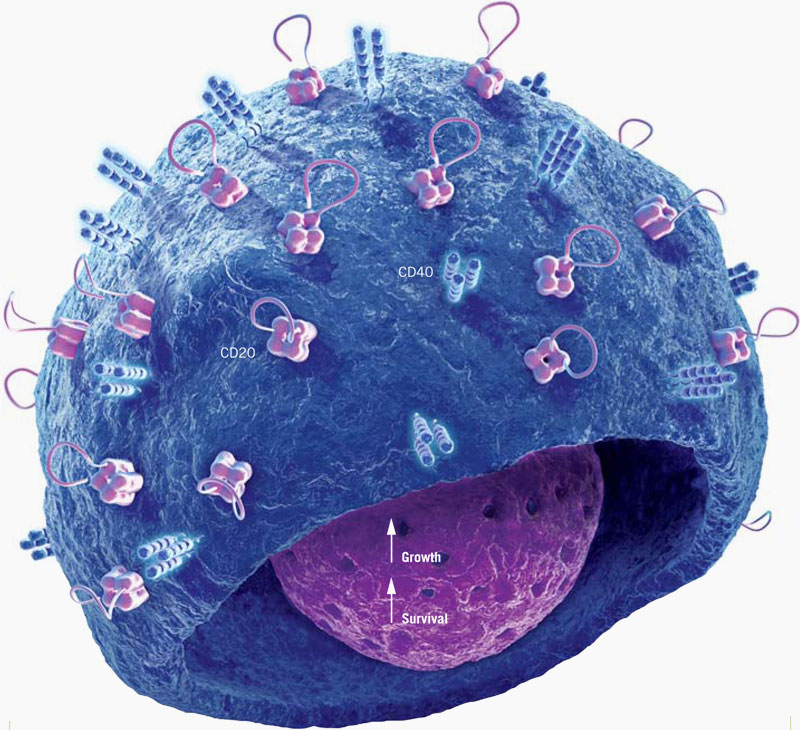
\includegraphics[height=50mm]{Cover/coverimage}  \end{center} % gráficos
 \vspace{5mm}
 
 %%% Titulo
\centering
\LARGE \textbf{Static Aplication Security Testing Tools}
\\ \vspace{10mm}
\Large SCOPE, IMPROVEMENTS AND FUTURE APPLICATIONS
\\ \vspace{15mm}
%\\ \vspace{25mm}  % NO SUBTITLE
\Large \textbf{Sofia Oliveira Reis} \\
\vspace{4cm}

\begin{minipage}{\textwidth}
\begin{tabularx}{\textwidth}{ l }
\large \textbf{Supervisor} : Rui Maranhão Abreu\\
 \large \textbf{Co-Supervisor} :  João Ferreira\\
\end{tabularx}

\end{minipage}
%
\\ \vspace{27mm}
%\vspace{12mm}
\centering
\large \textbf{Thesis specifically prepared to obtain the PhD Degree in}\\
\large Computer Science and Engineering\\
%\\ \vspace{2mm}
\vspace{18mm}
\Large \textbf{Draft}
 
\vspace{15mm}

\large \textbf{\todaythesis\today} \\
% \large \textbf{December 2017} \\
\let\thepage\relax
\end{flushleft}
\pagebreak
 
%\setcounter{page}{1} \pagenumbering{Alph}

% Add PDF bookmark 
\pdfbookmark[0]{Title}{Title}

%%% LOGO
\thispagestyle{empty}
\begin{flushleft} ~\\ \vspace{-12mm} \hspace{-12mm}  
\includegraphics[width=50mm]{Cover/istlogo} 
 
 %%% Instituição
\centering
\LARGE \textbf{UNIVERSIDADE DE LISBOA \\ INSTITUTO SUPERIOR TÉCNICO}
%%% espaço sem gráficos
\vspace{30mm}

%%% Optional Image
%\vspace{10mm}
%~\\ \vspace{50mm} % gráficos
%\\ \begin{center} 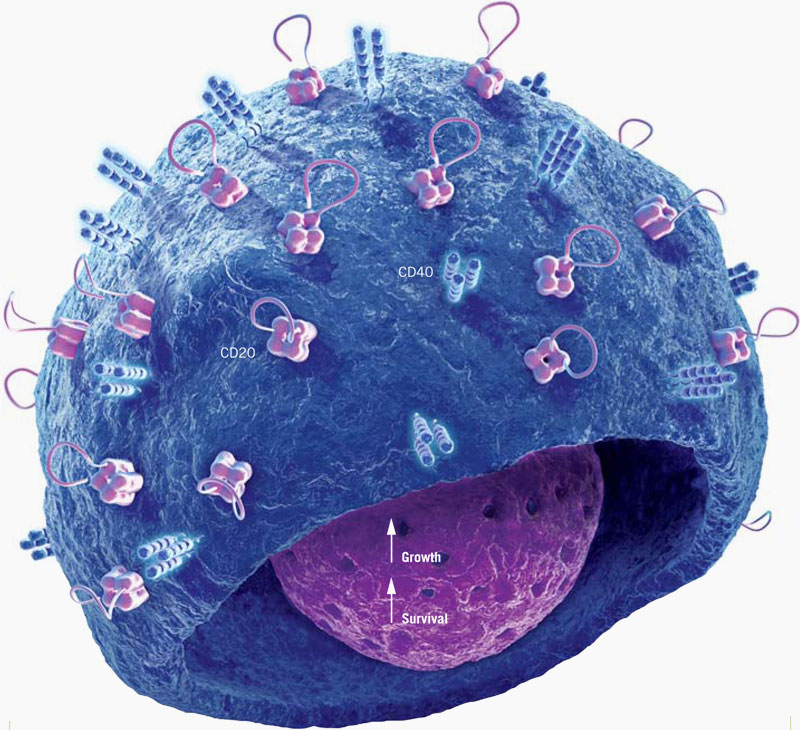
\includegraphics[height=50mm]{Cover/coverimage}  \end{center} % gráficos
 \vspace{5mm}
 
 %%% Titulo
\centering
\LARGE \textbf{Título da Tese que descreve o objeto de estudo.}
\\ \vspace{10mm}
\Large Subtítulo Opcional
\\ \vspace{15mm}
%\\ \vspace{25mm}  % NO SUBTITLE
\Large \textbf{Nome completo} \\
\vspace{4cm}

\begin{minipage}{\textwidth}
\begin{tabularx}{\textwidth}{ l @{ } l }
\large \textbf{Orientador} : & \textbf{Doutor} Nome completo\\
 \large \textbf{Co-Orientador} :  & \textbf{Doutor} Nome completo\\
 %&    ~~~~~~~~~~~~~~~~~~~~~~~~~~ large name\\
\end{tabularx}

\end{minipage}
%
\\ \vspace{27mm}
%\vspace{12mm}
\centering
\large \textbf{Tese especialmente elaborada para a obtenção do grau de Doutor em}\\
\large Engenharia Mecânica\\
%\\ \vspace{2mm}
\vspace{18mm}
\Large \textbf{Tese Provisória}
 
\vspace{15mm}

%\large \textbf{\todaythesis\today} \\
\large \textbf{November 2017} \\
\let\thepage\relax
\end{flushleft}
\pagebreak

%%%----------FINAL --- uncomment all code bellow and comment code above.
%\setcounter{page}{1} \pagenumbering{Alph}

% Add PDF bookmark 
\pdfbookmark[0]{Title}{Title}

%%% LOGO
\thispagestyle{empty}
\begin{flushleft} ~\\ \vspace{-12mm} \hspace{-12mm}  
\includegraphics[width=50mm]{Cover/istlogo} 
 
 %%% Instituição
\centering
\LARGE \textbf{UNIVERSIDADE DE LISBOA \\ INSTITUTO SUPERIOR TÉCNICO}
%%% espaço sem gráficos
\vspace{30mm}

%%% Optional Image
%\vspace{10mm}
%~\\ \vspace{50mm} % gráficos
%\\ \begin{center} 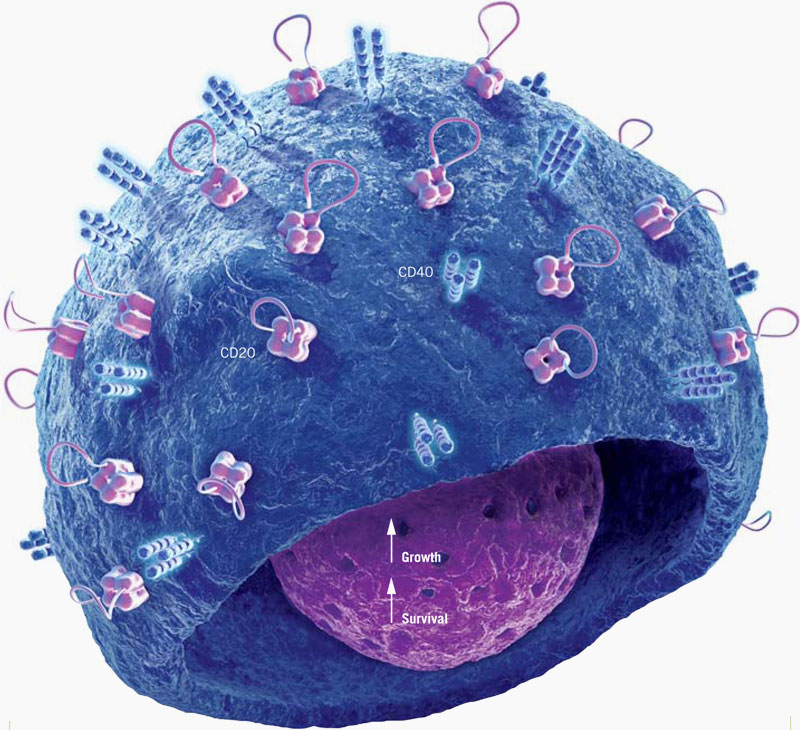
\includegraphics[height=50mm]{Cover/coverimage}  \end{center} % gráficos
 \vspace{5mm}
 
 %%% Titulo
\centering
\LARGE \textbf{Title of the Thesis that describes the main work done}
%\\ \vspace{10mm}
%\Large Optional Subtitle
%\\ \vspace{15mm}
\\ \vspace{25mm}  % NO SUBTITLE
\LARGE \textbf{Full Name} \\
\vspace{3cm}

\begin{minipage}{\textwidth}
\begin{tabularx}{\textwidth}{ l @{ } l }
\textbf{Supervisor} : & \textbf{Doctor full name}\\
\textbf{Co-Supervisor} :  & \textbf{Doctor full name}\\
\end{tabularx}

\end{minipage}
%
\\ \vspace{20mm}
%\vspace{12mm}
\centering\LARGE
\textbf{Thesis approved in public session to obtain the PhD Degree in Mechanical Engineering}\\
%\textbf{Mechanical Engineering}\\
\vspace{8mm}
\LARGE \textbf{Jury final classification:  Pass}\\
%\\ \vspace{2mm}
 
\vspace{20mm}

%\large \textbf{\todaythesis\today} \\
\LARGE \textbf{2019} \\
\let\thepage\relax
\end{flushleft}
\pagebreak
 
%%\setcounter{page}{1} \pagenumbering{Alph}

% Add PDF bookmark 
\pdfbookmark[0]{Title}{Title}

%%% LOGO
\thispagestyle{empty}
\begin{flushleft} ~\\ \vspace{-12mm} \hspace{-12mm}  
\includegraphics[width=50mm]{Cover/istlogo} 
 
 %%% Instituição
\centering
\LARGE \textbf{UNIVERSIDADE DE LISBOA \\ INSTITUTO SUPERIOR TÉCNICO}
%%% espaço sem gráficos
\vspace{30mm}

%%% Optional Image
%\vspace{10mm}
%~\\ \vspace{50mm} % gráficos
%\\ \begin{center} 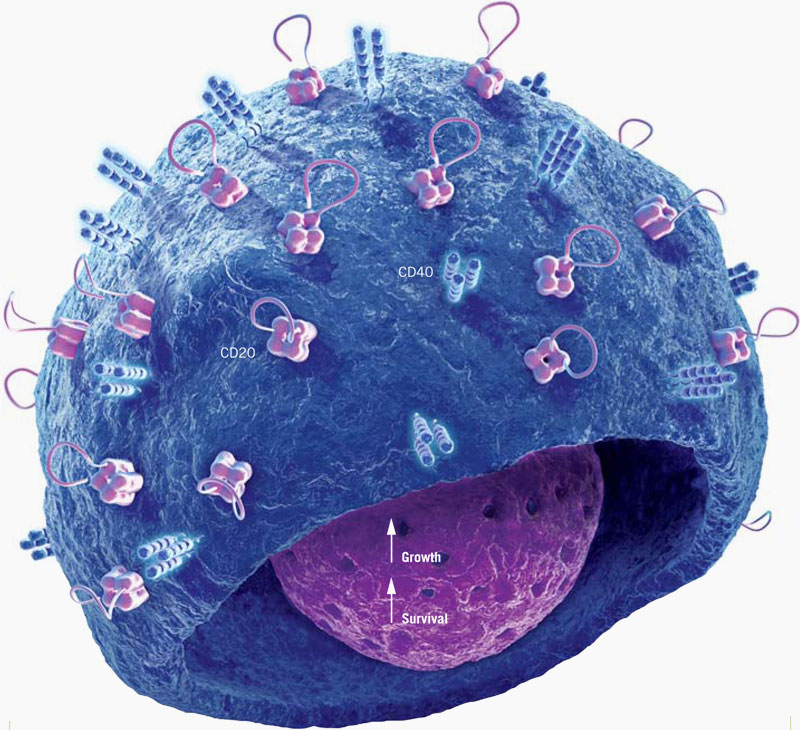
\includegraphics[height=50mm]{Cover/coverimage}  \end{center} % gráficos
 \vspace{5mm}
 
 %%% Titulo
\centering
\LARGE \textbf{Título da Tese que descreve o objeto de estudo}
\\ \vspace{10mm}
\Large Subtítulo Opcional
\\ \vspace{15mm}
%\\ \vspace{25mm}  % NO SUBTITLE
\LARGE \textbf{Nome completo} \\
\vspace{4cm}

\begin{minipage}{\textwidth}
\begin{tabularx}{\textwidth}{ l @{ } l }
\Large \textbf{Orientador} : & \textbf{Doutor Nome completo}\\
 \Large \textbf{Co-Orientador} :  & \textbf{Doutor Nome completo}\\
 %&    ~~~~~~~~~~~~~~~~~~~~~~~~~~ large name\\
\end{tabularx}

\end{minipage}
%
\\ \vspace{20mm}
%\vspace{12mm}
\centering
\Large \textbf{Tese aprovada em provas públicas para a obtenção do grau de Doutor em Engenharia Mecânica}\\
%\\ \vspace{2mm}
\vspace{8mm}
\Large \textbf{Qualificação atribuída pelo Júri: Aprovado}
%\Large \textbf{Qualificação atribuída pelo Júri: Aprovado com Distinção.}
 
\vspace{20mm}

%\large \textbf{\todaythesis\today} \\
\large \textbf{2019} \\
\let\thepage\relax
\end{flushleft}
\pagebreak
 
%\clearpage
%\thispagestyle{empty}
%\cleardoublepage
%\setcounter{page}{1} \pagenumbering{Alph}

% Add PDF bookmark 
\pdfbookmark[0]{Title}{Title}

%%% LOGO
\thispagestyle{empty}
\begin{flushleft} ~\\ \vspace{-12mm} \hspace{-12mm}  
\includegraphics[width=50mm]{Cover/istlogo} 
 
 %%% Instituição
\centering
\LARGE \textbf{UNIVERSIDADE DE LISBOA \\ INSTITUTO SUPERIOR TÉCNICO}
%%% espaço sem gráficos
\vspace{10mm}

%%% Optional Image
%\vspace{10mm}
%~\\ \vspace{50mm} % gráficos
%\\ \begin{center} 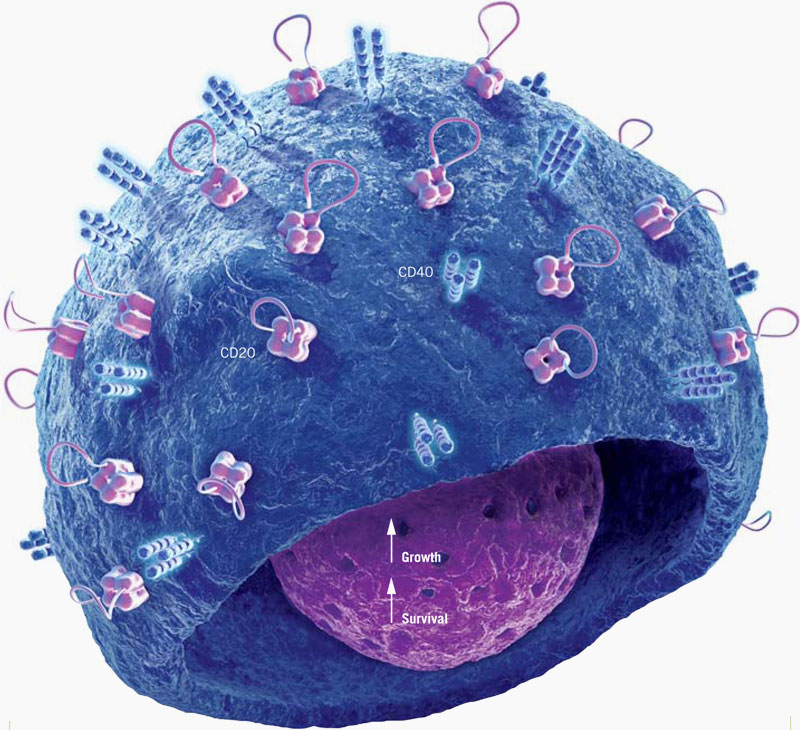
\includegraphics[height=50mm]{Cover/coverimage}  \end{center} % gráficos
% \vspace{5mm}
 
 %%% Titulo
\centering
\Large \textbf{Thesis Title that describes the main work done}
%\\ \vspace{10mm}
%\Large Optional Subtitle
%\\ \vspace{15mm}
\\ \vspace{8mm}  % NO SUBTITLE
\Large\textbf{Full Name} \\
\vspace{8mm}

%Advisors
\Large %letter size for advisers
\begin{minipage}{\textwidth}
\begin{tabularx}{\textwidth}{ l @{ } l }
 \textbf{Supervisor} : & \textbf{Doctor full Name}\\
 \textbf{Co-Supervisor} :  &  \textbf{Doctor full Name}\\
\end{tabularx}
\end{minipage}
\\ \vspace{8mm}
\centering
\Large \textbf{Thesis approved in public session to obtain the PhD Degree in}\\
\Large \textbf{Mechanical Engineering}\\
\vspace{5mm}
\Large \textbf{Jury final classification:  Pass}\\
%\\ \vspace{2mm}
 
\vspace{8mm}
%Juri
\Large \textbf{Jury}\\
\vspace{2mm}
\raggedright\Large \textbf{Chairperson :}  \textbf{Doctor full name of the department president, Instituto Superior Técnico, Universidade de Lisboa;}\\
\Large \textbf{Members of the Committee :}\\ %\vspace{3mm}
%\hspace{1cm}\textbf{Doctor} João Eduardo de Barros Teixeira Borges, Instituto Superior Técnico, Universidade de Lisboa;
%\hspace{1cm}
\vspace{2mm}
\begin{minipage}{\textwidth}
\begin{tabularx}{1.1\textwidth}{ l @{ } p{0.9\textwidth} }
~~~ & \textbf{Doctor full Name, Instituto Superior Técnico, Universidade de Lisboa;}\\
 & \textbf{Doctor full Name    , Faculdade de Ciências e Tecnologia, Universidade Nova de Lisboa;}\\
 & \textbf{Doctor full Name, Instituto Superior Técnico, Universidade de Lisboa;}\\
 & \textbf{Doctor full Name, another university;}\\
 & \textbf{Doctor full Name, Institute, University.}\\
\end{tabularx}
\end{minipage}\\
\centering
\vspace{5mm}\Large \textbf{Funding Institutions - Fundação para a Ciência e a Tecnologia}\\
%
\vspace{10mm}

%\large \textbf{\todaythesis\today} \\
\Large \textbf{2019} \\
\let\thepage\relax
\end{flushleft}
\pagebreak
 
%%\setcounter{page}{1} \pagenumbering{Alph}

% Add PDF bookmark 
\pdfbookmark[0]{Title}{Title}

%%% LOGO
\thispagestyle{empty}
\begin{flushleft} ~\\ \vspace{-12mm} \hspace{-12mm}  
\includegraphics[width=50mm]{Cover/istlogo} 
 
 %%% Instituição
\centering
\LARGE \textbf{UNIVERSIDADE DE LISBOA \\ INSTITUTO SUPERIOR TÉCNICO}
%%% espaço sem gráficos
\vspace{10mm}

%%% Optional Image
%\vspace{10mm}
%~\\ \vspace{50mm} % gráficos
%\\ \begin{center} 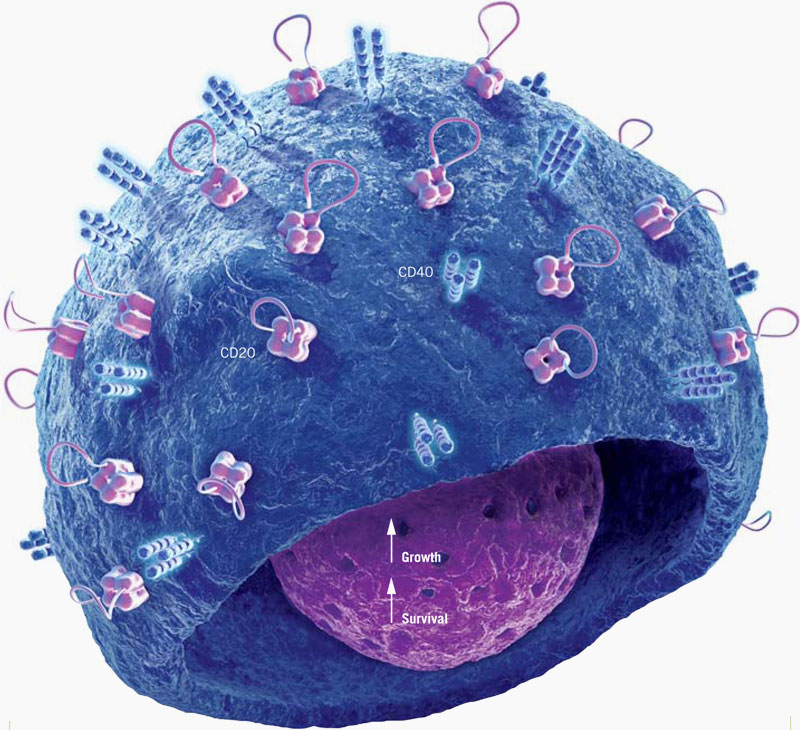
\includegraphics[height=50mm]{Cover/coverimage}  \end{center} % gráficos
 %\vspace{5mm}
 
 %%% Titulo
\centering
\Large \textbf{Título da Tese que descreve o objeto de estudo}
%\\ \vspace{2mm}
%\Large Subtítulo Opcional
\\ \vspace{8mm}
%\\ \vspace{25mm}  % NO SUBTITLE
\Large \textbf{Nome completo} \\
\vspace{8mm}

%Orientadores
\Large
\begin{minipage}{\textwidth}
\begin{tabularx}{\textwidth}{ l @{ } l }
\textbf{Orientador} : & \textbf{Doutor Nome completo}\\
\textbf{Co-Orientador} :  & \textbf{Doutor Nome completo}\\
 %&    ~~~~~~~~~~~~~~~~~~~~~~~~~~ large name\\
\end{tabularx}
\end{minipage}
\\ \vspace{8mm}
\centering
\Large \textbf{Tese aprovada em provas públicas para a obtenção do grau de Doutor em}\\
\Large Engenharia Mecânica\\
\vspace{5mm}
\Large \textbf{Qualificação atribuída pelo Júri: Aprovado}
%\Large \textbf{Qualificação atribuída pelo Júri: Aprovado com Distinção.}
 
\vspace{8mm}
%Juri
\Large \textbf{Júri}\\
\vspace{2mm}
\raggedright\Large \textbf{Presidente :}  \textbf{Doutor Nome Completo, Instituto Superior Técnico, Universidade de Lisboa;}\\
\Large \textbf{Vogais :}\\
\vspace{2mm}
\begin{minipage}{\textwidth}
\begin{tabularx}{1.1\textwidth}{ l @{ } p{0.9\textwidth} }
~~~ & \textbf{Doutor Nome Completo, Instituto Superior Técnico, Universidade de Lisboa;}\\
 & \textbf{Doutor Nome Completo, Faculdade de Ciências e Tecnologia, Universidade Externa;}\\
 & \textbf{Doutor Nome Completo, Instituto Superior Técnico, Universidade de Lisboa;}\\
 & \textbf{Doutor Nome Completo, Instituto Superior Técnico, Universidade de Lisboa;}\\
 & \textbf{Doutor Nome Completo, Instituto Superior ..., Universidade Externa.}\\
\end{tabularx}
\end{minipage}\\
\centering
\vspace{5mm}\Large \textbf{Instituições Financiadoras -\\ Fundação para a Ciência e a Tecnologia}\\
%
\vspace{10mm}

%\large \textbf{\todaythesis\today} \\
\Large \textbf{2019} \\
\let\thepage\relax
\end{flushleft}
\pagebreak
 
%%\clearpage


%%-------------------------------------
\clearpage
% Since I am using double sided pages, the second page should be white.
% Remember that when delivering the dissertation, IST requires for the cover to appear twice.

\thispagestyle{empty}
\cleardoublepage

\setcounter{page}{1} \pagenumbering{roman} % --- Start with Roman numbering ---

\baselineskip 18pt % line spacing: -12pt for single spacing
                   %               -18pt for 1 1/2 spacing
                   %               -24pt for double spacingnts}
                   
 %%%% Initial Chapters
 \selectlanguage{english}
\begin{abstract}

The Objective of this Work ... (English)

\end{abstract}
\begin{keywords}
Keywords (English)
\end{keywords}
\clearpage
\thispagestyle{empty}
\cleardoublepage
\selectlanguage{portuguese}
\begin{resumo}

O objectivo deste trabalho ... (Português)

\end{resumo}
\begin{palavraschave}
Palavras-Chave (Português)
\end{palavraschave}
\clearpage
\thispagestyle{empty}
\cleardoublepage

\pdfbookmark{Acknowledgments}{Acknowledgments}
\begin{acknowledgments} 

I would like to thank the Academy, bla bla bla..

\end{acknowledgments}
\clearpage
\thispagestyle{empty}
\cleardoublepage
\thispagestyle{empty}
\hbox{} \vfill
\begin{flushright}
\small \textit{\textbf{Anyone who has never made a mistake has never tried anything new.}}
\\ \vspace{2mm}  
\scriptsize Albert Einstein
\end{flushright}

\clearpage
\thispagestyle{empty}
\cleardoublepage % --- Citation (optional) ---
%% Use Main document Language
\selectlanguage{english}
%-- ! --> Usar 'portuguese' para versão portuguesa.
%% ------
% This is required for the fancy chapters
\dominitoc
\dominilof
\dominilot

%%%%%%%%%%%%%%%%%%%%%%%%%%%%%%%%%%%%%%%%%%%%%%%%%%%%%%%%%%%%%%%%%%%%%%
% List of contents
%\renewcommand{\baselinestretch}{1}
\pdfbookmark[0]{Index}{index}
\pdfbookmark[1]{Contents}{toc}
\tableofcontents
% \contentsline{chapter}{References}{\pageref{bib}}
\clearpage
\thispagestyle{empty}
\cleardoublepage
%\renewcommand{\baselinestretch}{1.5}
%%%%%%%%%%%%%%%%%%%%%%%%%%%%%%%%%%%%%%%%%%%%%%%%%%%%%%%%%%%%%%%%%%%%%%
% List of figures
\pdfbookmark[1]{List of Figures}{lof}
\listoffigures
\clearpage
\thispagestyle{empty}
\cleardoublepage

%%%%%%%%%%%%%%%%%%%%%%%%%%%%%%%%%%%%%%%%%%%%%%%%%%%%%%%%%%%%%%%%%%%%%%
% List of tables
\pdfbookmark[1]{List of Tables}{lot}
\listoftables
\clearpage
\thispagestyle{empty}
\cleardoublepage

% %%%%%%%%%%%%%%%%%%%%%%%%%%%%%%%%%%%%%%%%%%%%%%%%%%%%%%%%%%%%%%%%%%%%%%
% % List of algorithms
% Requires packages algorithmic, algorithm
% \pdfbookmark[1]{List of Algorithms}{loa}
% \listofalgorithms
% \cleardoublepage
%\acresetall
%% Remain list of table titles are set manualy
% %%%%%%%%%%%%%%%%%%%%%%%%%%%%%%%%%%%%%%%%%%%%%%%%%%%%%%%%%%%%%%%%%%%%%%
 % List of acronyms
\pdfbookmark[1]{List of Acronyms}{loac}
%\chapter*{Abbreviations}

%GLOSSARIO de Acrónimos
\printglossary[type=\acronymtype]

\clearpage
\thispagestyle{empty}
\cleardoublepage




%%%%%%%%%%%%%%%%%%%%%%%%%%%%%%%%%%%%%%%%%%%%%%%%%%%%%%%%%%%%%%%%%%%%%%%
% List of symbols
\pdfbookmark[1]{List of Symbols}{los}

\listofsymbols

%GLOSSARIO
\printglossary[type=\acronymtype]

\clearpage
\thispagestyle{empty}

\cleardoublepage
% Pages number is starting now with arabic style... until now it was on roman mode
\pagenumbering{arabic} \setcounter{page}{1}
\baselineskip 18pt %changed to glossaries
%
%		Notation
%
%
\pdfbookmark[1]{Notation}{los}

%%%%%%%  Notação dividida em glossários
\chapter*{Notation}

\setglossarysection{section}
%\setglossarystyle{list}
\printglossary[type=latinletters, style=mylist,title=Latin Letters]
\printglossary[type=greekletters]
\printglossary[type=subscripts]
\printglossary[type=ratesratios]

%\glsaddall  
\forallglsentries{\thislabel}%
{%
  \ifglsused{\thislabel}{}{\glsadd[format=ignore]{\thislabel}}%
}


%%%%%%  Notação, modo antigo: secções são subentradas

%\input{./00.Definitions/Notation-List_opt.tex}
%
%%\printglossary[type=symbolslist,style=mylist,title=Notation]
%\printglossary[style=mylist,title=Notation]  
%%\printglossaries


%%%%%%%%%%%%%%%%%  Final da Página de Notação

\clearpage
\thispagestyle{empty}

\cleardoublepage
% Pages number is starting now with arabic style... until now it was on roman mode
\pagenumbering{arabic} \setcounter{page}{1}
\baselineskip 18pt
%% Use Main document Language
\selectlanguage{english}
%-- ! --> Usar 'portuguese' para versão portuguesa.
%% Define the title of Chapter Table of Contents
\mtcsettitle{minitoc}{Contents}
%% ------
\pagestyle{documentsimple}%Simple head
% %%%%%%%%%%%%%%%%%%%%%%%%%%%%%%%%%%%%%%%%%%%%%%%%%%%%%%%%%%%%%%%%%%%%%%
% The Introduction:
% %%%%%%%%%%%%%%%%%%%%%%%%%%%%%%%%%%%%%%%%%%%%%%%%%%%%%%%%%%%%%%%%%%%%%%
\fancychapter{Introduction}
\label{cap:int}

\section{Motivation}
\label{sec:int_motivation}

Motivation Section.
\section{State of The Art}
\label{sec:int_state}

State of The Art Section.

\subsection{Dummy Subsection A}
\label{subsec:subsectiona}

State of Art Subsection A

\subsection{Dummy Subsection B}
\label{subsec:subsectionb}

State of Art Subsection B


\section{Original Contributions}
\label{sec:int_contributions}

Contributions Section.
\section{Thesis Outline}
\label{sec:int_outline}

Outline Section.

\cleardoublepage
% %%%%%%%%%%%%%%%%%%%%%%%%%%%%%%%%%%%%%%%%%%%%%%%%%%%%%%%%%%%%%%%%%%%%%%
% Dummy Chapter:
% %%%%%%%%%%%%%%%%%%%%%%%%%%%%%%%%%%%%%%%%%%%%%%%%%%%%%%%%%%%%%%%%%%%%%%

% %%%%%%%%%%%%%%%%%%%%%%%%%%%%%%%%%%%%%%%%%%%%%%%%%%%%%%%%%%%%%%%%%%%%%%
% The Introduction:
% %%%%%%%%%%%%%%%%%%%%%%%%%%%%%%%%%%%%%%%%%%%%%%%%%%%%%%%%%%%%%%%%%%%%%%
\fancychapter{Static Application Security Testing: Scope and Opportunities}
\label{cap:chapter}

\textit{Catalog of academic and non-academic SAST tools.}

\section{Section A}
\label{sec:sectiona}

\subsection{Subsection A}
\label{subsec:subasectionA}

This would be a citation \cite{dummy}.

The \gls{cop} defines the performance of the machine.
% The first time you use this, the acronym will be written in full with the acronym in parentheses: supernova (SN). At later times it will just print the acronym: SN.

Heat Pump's performance is given by the \gls{cophp}, a \gls{cop} for heat pumps.

\section{Section B}
\label{sec:sectionb}

\subsection{Subsection A}
\label{subsec:subasectionB}



\cleardoublepage

% %%%%%%%%%%%%%%%%%%%%%%%%%%%%%%%%%%%%%%%%%%%%%%%%%%%%%%%%%%%%%%%%%%%%%%
% Dummy Chapter:
% %%%%%%%%%%%%%%%%%%%%%%%%%%%%%%%%%%%%%%%%%%%%%%%%%%%%%%%%%%%%%%%%%%%%%%

% %%%%%%%%%%%%%%%%%%%%%%%%%%%%%%%%%%%%%%%%%%%%%%%%%%%%%%%%%%%%%%%%%%%%%%
% The Introduction:
% %%%%%%%%%%%%%%%%%%%%%%%%%%%%%%%%%%%%%%%%%%%%%%%%%%%%%%%%%%%%%%%%%%%%%%
\fancychapter{SAST Testing and Validation}
\label{cap:chapter}

\textit{Present the chapter content.}

\section{Introduction}~\label{sec:intro}

% the problems of patch management 
% why do we need to patch 
% vulnerabilities faster -- EQUIFAX
Delays in deploying patches to known software security vulnerabilities 
have been the cause of major cybersecurity attacks~\cite{windows-cyberattack,failed-to-deploy-patch,hacker-news-patches,CISA-ALERT,non-applied-patches}. 
A practical example with major financial and reputation losses was the Equifax breach~\cite{failed-to-deploy-patch}: a failure to patch a 2-month-old critical bug in Apache Struts, which led to a sensitive data breach that impacted more than 143 million US consumers~\cite{EQUIFAX-1}. 
Timely patch management (i.e., the fast distribution and deployment 
of security fixes to users~\cite{SOFT-PATCH-MANAG-NIST,DBLP:conf/soups/LiRMMC19,10.5555/3488905.3488919,10.5555/3337432.3337437}) is one of the most effective and widely recognized strategies for 
% reducing the users' exposure window~\cite{DBLP:journals/corr/abs-2001-09148} and 
protecting
software systems against  cyberattacks~\cite{DISSANAYAKE2022106771,SOFT-PATCH-MANAG-NIST}. Yet, one important challenge still prevails, the \emph{lack of efficient patch triage systems} to identify and prioritize security patches~\cite{Zhang2021AnIO, SSPatcher2022,hacker-news-patches,DBLP:conf/soups/LiRMMC19}: current processes are largely manual (time-consuming) and prone to ignore important bug fixes such as the one behind Equifax~\cite{failed-to-deploy-patch}. An ideal and effective patch management process should include an effective audit system to identify patches~\cite{hacker-news-patches}. A recent study showed that $56.7\%$ of the commit messages attached to security patches are documented poorly and hinder  triage systems tasks (e.g., detection, prioritization, and assessment)~\cite{10.1145/3593434.3593481}.  

\textbf{Problem: Poor quality security commit messages hinder patch triage systems.} Previous work focused on using 
patch metadata (e.g., commit message) and code changes 
to explore automated patch detection~\cite{SSPatcher2022,reis2017secbench,9678720,DBLP:journals/corr/abs-1806-05893}, concluded that software vulnerability management (SVM) techniques could not rely purely on metadata to detect software vulnerabilities
due to the often inaccurate and incomplete  data~\cite{DBLP:journals/corr/abs-1806-05893}. In fact, only $38\%$ of commit messages used to ``silently'' patch software vulnerabilities in the past included security-related words~\cite{9678720}. Silent fixes
are performed when the vendor patches a vulnerability  without mentioning its existence anywhere (e.g., release notes, commit message, and more)~\cite{9678720}. This practice naturally leads to less informative patch documentation and hinders triage systems awareness and effectiveness. While this practice is usually used to protect vendors and systems, it
also limits the general knowledge pool of people who actually understand the vulnerability and know how to exploit it, which leaves users and defenders unprotected and unaware. According to the CERT Coordinated Vulnerability Disclosure (CVD) guide, silent patches should be avoided since knowing the existence of vulnerabilities and their patches is often the key driver to effective patch deployment~\cite{Householder2020}. 

%%%% Importance of the problem
% Providing well-structured and quality documentation of security patches can improve the  understanding of these software vulnerabilities for researchers and developers, which can ultimately enable faster patch management~\cite{Zhang2021AnIO,Householder2020,SSPatcher2022,10.1145/3593434.3593481}. Software vulnerabilities are, on average, disclosed only one week after the patch release~\cite{10.1145/3133956.3134072}---leaving, again, users vulnerable and unaware. Therefore, making the information available earlier in the process is of utmost importance.

%%%% not sure how this part helps
% Yet, previous work succeeded in locating software vulnerabilities and their respective patches using manual validation~\cite{10.1109/MSR.2019.00064} or regular expressions~\cite{reis2017secbench, SSPatcher2022} over commit messages (i.e., some data in commit messages can in fact be leveraged for this task).

\textbf{Motivation:} 
Security commit messages (i.e., the commit messages attached to the code changes used to patch software vulnerabilities) can be cryptic~\cite{9678720}, hindering triage tasks. 
Table~\ref{tab:messages} shows examples of security commit messages (col. Message) used to document patches to known software vulnerabilities (col. VulnID) and the 
patch commit key (col. SHA). Message 1 (``.'') is an example of a cryptic message as it does not provide any information. From messages 2 and 3, it
is possible to infer that a defect in code is being fixed, but nothing 
more than that. Message 4 is an internet meme called ``Rickrolling''\footnote{``Rickrolling'' meme details at \url{https://knowyourmeme.com/memes/rickroll}}, usually used to prank people with the "Never Gonna Give You Up" song. Although funny, the message does not provide, again, any relevant information regarding the vulnerability and respective patch. Most of the cases presented would not be detected by triage systems leaving users unaware of the new patches and exposed to vulnerabilities. Message 5  
provides a brief description of the patch and some relevant information about it (e.g., it fixes a ``security issue'' related to ``passwords''). The respective code changes fix a potential buffer overrun vulnerability resulting from reading user-provided passwords and confirmations via command-line prompts. The patch fixes an ``Improper Authentication'' weakness (CWE-287) with a severity (CVSS) score of $8.4$ in $10$---which 
is not explicit in the message. This extra information could have helped
automated or even manual patch triage systems to prioritize this patch since it has high severity. 



\begin{table}[!t]
    \footnotesize
    \centering
    \begin{tabular}{ | p{0.01cm} | p{4.8cm} | p{1.5cm} | p{0.9cm} |} 
    \hline
     & \textbf{Commit Message} & \textbf{VulnID} & \textbf{SHA}\\\hline
        1 & \texttt{.} & CVE-2019-13568 & \href{https://github.com/GreycLab/CImg/commit/ac8003393569aba51048c9d67e1491559877b1d1}{ac80033} \\\hline
        2 & \texttt{Minor patch.} & OSV-2020-2108 & \href{https://github.com/simdjson/simdjson/commit/a8bf10ea5a0ea2553f07ac46744666c94d0085fc}{a8bf10e} \\\hline
        3 & \texttt{Code refactoring.} & GHSA-4fc4-4p5g-6w89 & \href{https://github.com/ckeditor/ckeditor4/commit/d158413449692d920a778503502dcb22881bc949}{d158413} \\\hline
        4 & \texttt{<scratchsig><script>location=
        'https:\/\/www.youtube.com\/watch?
        v=dQw4w9WgXcQ';<\/script><\/scratchsig>} & CVE-2020-15179 & \href{https://github.com//InternationalScratchWiki//wiki-scratchsig//commit//4160a39a20eebeb63a59eb7597a91b961eca6388}{4160a39} \\\hline
        5 & \texttt{Fixed security issues with passwords entered via a prompt} & CVE-2022-35928 & \href{https://github.com/paulej/AESCrypt/commit/68761851b595e96c68c3f46bfc21167e72c6a22c}{6876185} \\
    \hline
    \end{tabular}
    \caption{Examples of commit messages used to patch known software vulnerabilities.}
    \label{tab:messages}
\end{table}


\textbf{Study.} While some argue that security commit messages and patch release notes should be minimalist, others argue that the details are crucial to ensure triage systems effectiveness~\cite{SSPatcher2022,Zhang2021AnIO}, create trust amongst users~\cite{Householder2020}, and enable fast patch management~\cite{Zhang2021AnIO,Householder2020}. Therefore, we investigated the current status of security commit messages and answered the following questions: (1) what information is included in commit messages of public security patches; (2) are security engineers following best practices to produce security commit messages; and, 
(3) is the security community open to a new
standard for security commit messages.
In our work, we empirically analyzed $11036$ security commit messages by extracting key information (security words, vulnerability ID, weakness ID, severity, and more) with a customized named entity recognition (NER) tool.

\textbf{Results.} We found that $61.2\%$ of security commit messages include security-related words but lack key information such as the vulnerability ID, weakness ID, and severity. We were unable to extract any information from $8\%$ of the messages because (1) they were poorly documented, (2) their vocabulary was non-security related, or (3) they had misspelled words. Overall, security engineers poorly follow best practices to write general commit messages indicating that a set of new best practices for this task are needed. 

\textbf{Solution.} To address the challenges identified from our empirical analysis, we developed a structured and comprehensive convention called \texttt{SECOM} for writing security commit messages. We noticed 
security engineers sometimes follow standards to write general commit messages in security commit messages (e.g., Conventional Commits~\cite{convcom}). Therefore, we designed the standard
on top of best practices for writing generic commit messages to facilitate adoption. \texttt{SECOM} was designed according to (1) the results of the empirical analysis of historical commit messages and (2) validation of SECOM with the open-source security community. The standard was created with the aim of making the task of automated reasoning tools easier for patch detection (by adding a clear indicator for vulnerability fixes) and prioritization (by considering severity score and weakness type). 

\begin{figure}[!t]
    \centering
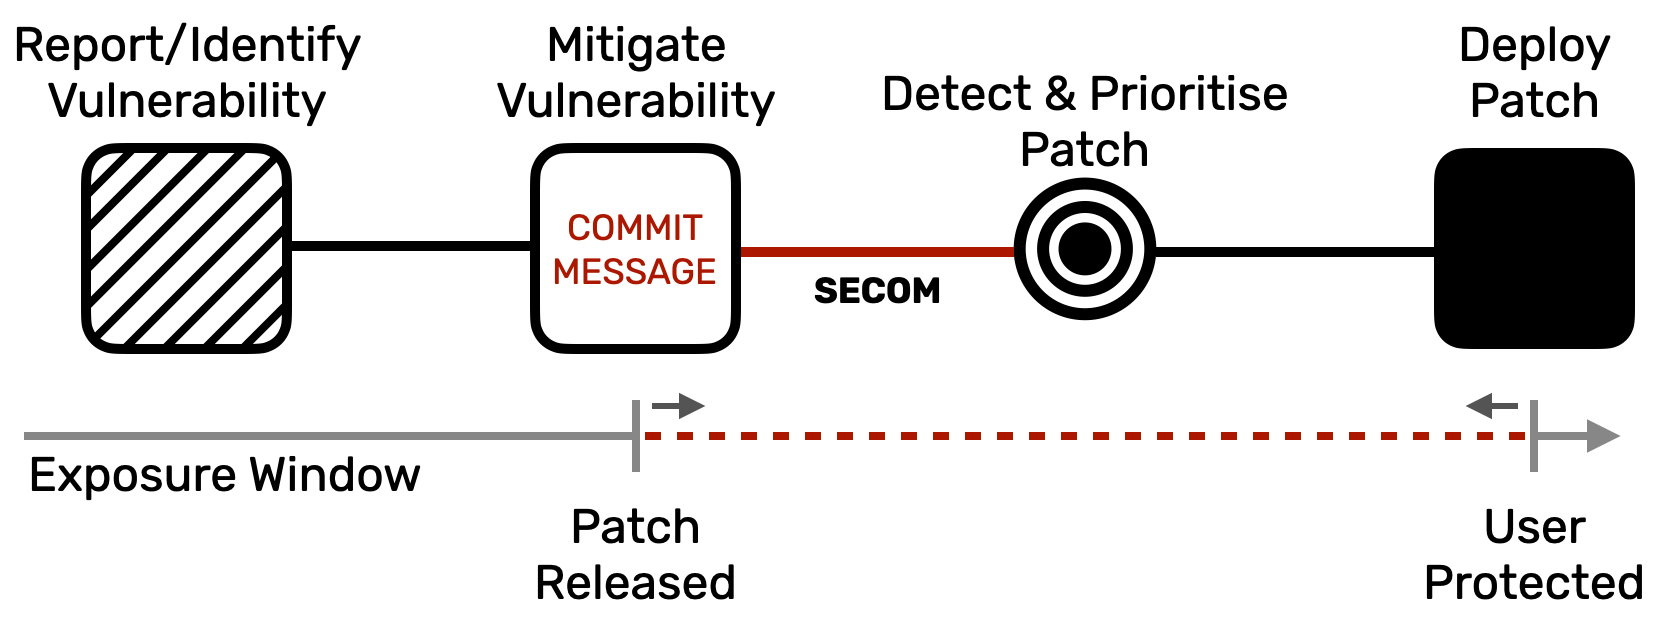
\includegraphics[width=\linewidth]{Figures/cycle.png}
    \caption{Problem and Solution illustration.}\label{fig:cycle}
\end{figure}

\textbf{Impact.} Figure~\ref{fig:cycle} shows where SECOM can help improve patch management processes: well-documented commit messages can be detected by triage systems and shorten the time between the patch is released and deployed. 
From a research perspective, detecting and assessing vulnerabilities continues to be a main challenge in vulnerability prediction due to the scarcity
and poor quality of curated data~\cite{9448435}. 
\texttt{SECOM} can be an important tool in softening this issue since it has the potential to improve the quality of data for future dataset creation. More than 2k security commit messages have been produced with the \texttt{SECOM} convention\footnote{\url{https://github.com/JLLeitschuh/security-research/issues/8}} so far.
We are aware of the challenges that come from too much transparency, and we want to guide the community to make proper and careful use of this new standard. Therefore, in this paper, we also provide guidelines on using \texttt{SECOM} carefully.
% Efforts to automate compliance validation and recommendations are also mentioned in this paper. 

\textbf{Contribution.} In summary, our contributions are the following: 
(1) an empirical analysis of security commit messages and best practices application; (2) a standard for security commit messages, called SECOM; and, (3) guidelines on how to write better security commit messages and apply the convention carefully.



\section{Background}~\label{sec:background}

This section provides background information on the Named Entity Recognition (NER) theory, the approach used to extract key information from security commit messages.

\subsection{Named Entity Recognition}~\label{sec:ner}

\begin{figure}[t!]
\hspace*{-0.25cm}\centering
    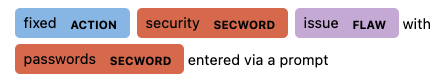
\includegraphics[width=\linewidth]{Figures/application.png}
    \caption{Named Entity Recognition (NER) application example for a security commit message.}\label{fig:application}
\end{figure}

Named Entity Recognition (NER) is a form of
Natural Language Processing (NLP)---also referred to as entity chunking, extraction, or identification. It is the task of identifying and extracting key information, called \emph{entities}, from unstructured data (in this case, text)~\cite{9039685, mikheev-etal-1999-named, lample-etal-2016-neural}.

An \emph{entity} can be any word or bag of words that refer to the same \emph{entity category}. For instance, different names of companies ``Netflix'', ``Google'' or ``Apple'' are entities that belong to the \emph{Company} category. 
NER requires the design of specific entity categories and the respective entity values, which relies on good domain knowledge. 
NER has been applied to different domains in the past, such as biomedical sciences~\cite{hakala-pyysalo-2019-biomedical}, pharmacology~\cite{gonzalez-agirre-etal-2019-pharmaconer}, and even security. 

\subsection{Named Entity Recognition in Security}~\label{sec:ner}

Previous work used NER to extract product names and versions from vulnerability reports~\cite{10.5555/3361338.3361399}. In our empirical analysis, we designed a group of category entities that are usually found in security commit messages and used a customized NER tool for security to extract key information (or entities) from commit messages used to patch software vulnerabilities.
Figure~\ref{fig:application}
shows an example of how we applied NER to security commit messages. Our tool extracted 4 different entities (``fixed'', ``security'', ``issue'', ``passwords'') for 3 different category entities (``ACTION'', ``SECWORD'', ``FLAW''). Only relevant words are extracted and tagged with their respective category entities, which is crucial for a  better understanding of the meaningful information provided in security commit messages.


\section{Research Questions}\label{sec:research_questions}

We use a mixed-method approach to answer three research questions. The first two research questions, RQ1 and RQ2, are answered by a cross-sectional empirical study of existing security commit messages. The third research question, RQ3, is answered through a survey study. 

\subsubsection*{\textbf{RQ1. What information is included in
the commit messages of public security patches?}}

Previous work has shown that SVM techniques can not rely purely on commit messages due to poor data quality~\cite{DBLP:journals/corr/abs-1806-05893}.
A study on vulnerabilities patched ``silently'' showed that only $38\%$ of commit messages used to fix vulnerabilities included security-related words~\cite{9678720}. 
But some previous approaches have managed to find some relevant natural language information in commit messages and perform security patch detection~\cite{reis2017secbench,10.1145/3106237.3117771,SSPatcher2022,DBLP:journals/corr/abs-1807-02458,10.1145/3593434.3593481}. The question 
that remains is what information is being mentioned in the commit messages
of security patches.

% \textbf{RQ2. Are there any guidelines available to
% produce security commit messages?} One way to produce quality 
% commit messages is by following best practices or guidelines~\cite{Tian_2022, convcom,linus,atomic}. In this part
% of the study, we searched for potential 
% standards to write commit messages of software security patches.

\textbf{RQ2. Do security engineers follow best practices to write security commit
messages?} 
One way to produce quality 
commit messages is by following best practices or guidelines~\cite{Tian_2022, convcom,linus,atomic}. However, researchers found that $44\%$ of commit messages need improvement~\cite{Tian_2022}. 
Our research revealed a lack of standards for writing security commit messages. Instead,
we found standards and guidelines for generic commit messages~\cite{convcom, linus, goodcommit}.
%In this part of our empirical analysis, 
Therefore, we explored if available guidelines or standards 
were being used and how they could be leveraged to create more structured and complete commit messages for security patches.

\emph{\textbf{RQ3. How open is the security community to a new standard for security commit messages?}}. Standards are usually seen as a burden or with resistance. However, in order to fix challenges, we need to create them. Therefore, we validated our convention with the open-source security community (Open Source
Security Foundation).


\section{Study of Existing Security Commit Messages}\label{sec:study_design}

This section describes an exploratory, cross-sectional empirical study of security commit messages collected from security patches for known vulnerabilities for answering RQ1 and RQ2. 


\subsection{Dataset Collection and Preprocessing} 

This section presents the steps taken to create a dataset of security commit messages.
All the tools used to collect and preprocess the data are available in our replication package. Our dataset considers data released until the 12th of August, 2022.
We collected security commit messages for our exploratory analysis by following the steps described below.

\subsubsection{Vulnerability Metadata Collection from Public Vulnerability Databases}
%
Public vulnerability databases, such as 
the National Vulnerability Database 
(NVD)~\cite{nvd}, and
the Open-Source Vulnerability (OSV) 
database~\cite{osv}, integrate documentation (or reports) for thousands of known vulnerabilities. Our dump of the OSV database includes a total of $30091$ vulnerability reports for open-source vulnerabilities from different ecosystems:
$28.6\%$ of the vulnerabilities were reported by GitHub Advisories, $25.7\%$ by  Linux, $11.1\%$ by PyPI,
$8.5\%$ by NPM, $7.8\%$ by OSS-Fuzz, and, the remaining $18.3\%$ by the rest of the
sources (e.g., Maven, RubyGems, Go,
and more). OSV only includes reports of vulnerabilities published after $2005$ (inclusive) 
and vulnerabilities reported by a restricted group of ecosystems. NVD includes reports of known vulnerabilities published since $1999$ and has no restrictions regarding the 
ecosystem (as far as we know). Therefore, we also considered the 
NVD database in our study. For NVD, we collected a total of $181614$ 
vulnerability reports. In total, we collected $211705$ vulnerability reports from both databases.


\begin{table*}[t!]
\footnotesize
    \centering
        \caption{Entity category names, rationale, and entity examples.} 
    \begin{tabular}{ | p{0.5cm} | p{1.4cm} | p{8.5cm} | p{5.5cm} |  p{0.5cm} | }
    \hline
         \textbf{Type} & \textbf{Category} & \textbf{Rationale} & \textbf{Entity Examples} & \textbf{Rules} \\\hline
        
        \multirow{5}{*}{SEC} & SECWORD & Security-relevant words are usually used to describe the vulnerability and respective fix (we used a large set of security-relevant words collected in previous work~\cite{10.1145/3133956.3134072,10.1145/3475716.3475781}). & ldap injection, crlf injection, improper validation, command injection, cross-site scripting, sanitize, bypass & 1719 \\\cline{2-5}
        
        & VULNID & Vulnerability IDs are used to identify vulnerabilities for different ecosystems in commit messages: CVE, GHSA, OSV, PyPI, etc. We crafted rules for the different IDs patterns. & GHSA-269q-hmxg-m83q, CVE-2016-2512, CVE-2015-8309, GHSA-9x4c-63pf-525f, OSV-2016-1 & 9
        \\\cline{2-5}
        
        & CWEID & Vulnerabilities usually belong to a weakness type. One common taxonomy used to classify security weaknesses is the Common Weakness Enumeration (CWE) one. Therefore, we crafted rules to detect CWE IDs. & CWE-119, CWE-20, CWE-79, CWE-189 & 2 \\\cline{2-5}
        
        & SEVERITY & Vulnerabilities usually have a severity assigned. & low, medium, high, critical & 4\\\cline{2-5}
        
        & DETECTION & Vulnerabilities are detected manually or using specific tools. & Manual, CodeQL, Coverity, OSS-Fuzz, libfuzzer & 8\\\hline
        
        \multirow{7}{*}{COM} & SHA & Commit hashes that reference older versions where the vulnerability was introduced (OSV Schema~\cite{osv-schema}). &  f8d773084564, 228a782c2dd0 & 2
        \\\cline{2-5}

        & ACTION  & A commit usually implies an action, in the case of security, 
        fixing a vulnerability (corrective maintenance). & fix, patch, change, add, remove, found, protect, update, optimize, mitigate & 18\\\cline{2-5}
        
        & FLAW & Fixing a security vulnerability usually implies fixing a flaw. & defect, weakness, flaw, fault, bug, issue & 10 \\\cline{2-5}
        
        & ISSUE & The GitHub issue/pull request number is sometimes referenced in the message and can provide more information on the vulnerability. & \#2, \#13245 & 1 \\\cline{2-5}
        
        & EMAIL & Contact e-mails of reviewers and authors usually appear after tags such as `Reported-by` and are important to know who to contact. & \url{johndoe123@gmail.com, catlover@yahooo.com, adventuretime@hotmail.com, supercool@outlook.com}$^1$  & 1\\\cline{2-5}
        
        & URL & Links to reports, blog posts, and bug-trackers references provide more information about the vulnerability. & \url{https://www.htbridge.ch/advisory/multiple_vulnerabilities_in_mantisbt.html} & 1\\\cline{2-5}
        
        & VERSION & Software versions are commonly referenced in commit messages. & 3.1.0, v3.2, v2.6.28, 1.6.3, 2.1.395 & 4\\\hline
        \multicolumn{5}{|l|}{\textbf{Type SEC}: Security specific entity categories; \textbf{Type COM}: Commit specific entity categories.} \\
        \multicolumn{5}{|l|}{$^1$\textbf{Artificial} e-mails generated automatically with ChatGPT for compliance with General Data Protection Regulation (GDPR).} \\\hline
    \end{tabular}
    \label{tab:entities-desc}
\end{table*}

\subsubsection{Collection and Preprocessing of References to Security Patches}

Each vulnerability report for both data sources includes a section referencing the fix (or patch), when 
available. An example of such a section can be found in~\cite{cve-example}. 

\textbf{Collection:} To get the commits involved in patching the security vulnerability, we filtered out all the vulnerability reports without references to commit links. We discovered that only $10010$ out of $30091$ OSV reports and $9953$ out of $181614$ NVD reports have references to commits 
(i.e., only $9\%$ of the vulnerability reports in those databases have fixes available). In addition, we observed that commits 
are usually available through GitHub, Bitbucket, SVN, and other services.
In this study, we only focus on vulnerability reports that include commits for fixes (i.e, security patches) available on GitHub, which accounts for over $80\%$ of the commits extracted from vulnerability 
reports. In total, we found references to GitHub fixes in $8670$ NVD reports and $9576$ OSV reports.

\textbf{Preprocessing:}
In order to collect the commit message of these commits, we used the GitHub API, which requires knowing the \textit{owner} of the repository that integrates the commit; the \textit{name of the repository}; and, the \textit{version} (or, \texttt{SHA} key) that included the vulnerability. 
However, sometimes due to the lack of precise information, we could not determine the data required to get the commit message (e.g., when the commit link had master instead of a specific \texttt{SHA} key). Thus, we could not ensure that the current version on master was the version where the vulnerability had been detected. Therefore, we removed all the vulnerability reports exhibiting  this issue,  which resulted in a total of $8405$ security patches for NVD ($3\%$ of data points) and $9466$ security patches for OSV ($1\%$ of data points). 

\textbf{Merging and Cleaning:}
Both data sources were merged after normalization into a dataset of $17871$ security patches while keeping the vulnerability reports metadata. Many vulnerabilities 
are reported in both NVD and OSV. 
Therefore, we found duplicates between both sources using different heuristics: 1) duplicated entries for security patches but with missing values for vulnerability score in one of the sources ($18\%$ of data points); 2) OSV reports contain a field called ``aliases'' which is a list of IDs of the same vulnerability in other databases. Therefore, we removed all the NVD entries ($19\%$ of data points) whose IDs where already in the aliases of OSV reports---OSV data was prioritized since previous research has shown that NVD has documentation problems and OSV is making an effort to fix those problems;
3) vulnerabilities fixed with the same 
patch, usually vulnerabilities that affect 
different codebases and therefore result in different vulnerability reports were also removed ($13\%$ of data points).
After removing the different types of duplicates, we end up with a dataset of $10254$ security patches.


\subsubsection{Collection and Preprocessing of Security Commit Messages}

Vulnerabilities can be fixed with one commit (single-commit patch) or multiple commits (multi-commit patch)---$88.6\%$ ($9083$) of the patches are single-commit patches while the other $11.4\%$ ($1170$) are multi-commit patches. From $10254$ security patches, we extracted a total of $11809$ security commits. GitHub metadata (including the commit message) was collected using the GitHub API. The commit messages were preprocessed in different ways: \textbf{(1)} A total of $334$  
commits (the equivalent to $160$ vulnerability reports) were \emph{no longer available} at the metadata collection time. Therefore, they were removed from the dataset. \textbf{(2)} We found \emph{duplicated commit messages} resulting from vulnerability reports with references to the vulnerability fix but deployed in different branches. One example is the GHSA-273r-mgr4-v34f\footnote{https://github.com/advisories/GHSA-273r-mgr4-v34f}, which references a commit per branch where the vulnerability was fixed. In these cases, since the commit messages are the same, we only kept one of the commits. Therefore, an extra $270$ commits were removed from the dataset---which left us with $11205$ security commit messages. \textbf{(3)} As in previous work~\cite{Tian_2022}, we searched for the same \emph{non-human generated message patterns} except when the original commit message was somehow attached to the commit message under analysis. For instance, in cases with the pattern ``<original commit message> (cherry picked from commit <commit>)'', the original commit message is attached at the beginning, and, in the ``merge pull request ... <original commit message>'' pattern, the original commit message is attached at the end. Therefore, we only remove non-human written messages that do not include any text generated by humans. One example is the \texttt{GHSA-3m93-m4q6-mc6v}\footnote{https://github.com/advisories/GHSA-3m93-m4q6-mc6v} advisory, which only references the cherry-picked commit. In addition to the patterns mentioned in~\cite{Tian_2022}, we also removed commit messages with pull request merges from dependabot and merge pull requests without any human text such as ``merge pull request from ghsa-g4hm-6vfr-q3wg''.
In summary, we found and removed a total of $126$ automated commit messages and kept $11079$ security commit messages. \textbf{(4)} We noticed some of the 
commit messages were not written in English. We ran \texttt{langdetect}\footnote{\texttt{langdetect}is an algorithm to infer the natural text language. It supports $55$ different text languages. Available at \url{https://github.com/Mimino666/langdetect}.} to infer the message's language. The model detected $1311$ ($11.8\%$) security commit messages as non-English. The tool can perform inaccurate predictions when evaluating too short or too ambiguous text. Therefore, we manually inspected the non-English messages to make sure we would not remove English and valid messages. 
After manual validation, we removed an extra $43$ non-English messages such as ``\begin{CJK*}{UTF8}{gbsn}导入mysql db时报错\end{CJK*}'' or ``\begin{CJK*}{UTF8}{gbsn}用户头像上传格式限制\end{CJK*}''.

\textbf{Results.} We successfully collected a total of $11036$ security commit messages (corresponding to $9943$ security patches). This dataset includes security commit messages used 
to document patches for $278$ different security weaknesses.


\subsection{Data Extraction (R1)}

This section explains the methodology used to extract key information from commit messages and answer our first research question. 

\subsubsection{Defining Domain-Specific Entities and Categories} 
% NER is an effective NLP technique to identify and tag entities based on specific rules or parameters~\cite{mikheev-etal-1999-named}. While 
% Text Classification looks at the characteristics of the text as a whole to draw conclusions (e.g., sentiment analysis), NER can provide more understanding of the text structure through the extraction of 
% key information (also known as entities). Previous work in the field has focused mainly on Text Classification~\cite{}. Both are important, since 

% To answer the question, ``\textbf{RQ1: Are security commit messages 
% informative?}'', w
We used NER (see Section~\ref{sec:ner}) to 
extract key information from security commit messages.
%
Firstly, we designed different entity categories: (1) security-specific or Type SEC, i.e., groups of words or bags-of-words that are common in security commit messages and security vulnerability reports (e.g., SECWORD, VULNID, CWEID, and more); and (2) commit-specific or Type COM (e.g., SHA, ACTION, FLAW, ISSUE, and more), i.e., groups of words or bags-of-words that are common in general commit messages. 
Table~\ref{tab:entities-desc} describes the different entity 
categories, the reason why each of them was considered (\textit{rationale}), entity examples, and the number of rules used to extract data each entity category---which can be fully inspected in our replication package or briefly in Table~\ref{tab:rules}. 

\subsubsection{Named Entity Extraction Pipeline} To extract the 
entities for each category, we used a Python library called Spacy\footnote{https://spacy.io/}---which provides end-to-end 
pipelines for several natural language processing tasks (e.g., NER). We built our own customized NER pipeline for security (see Figure~\ref{fig:parsing}). \textit{\textbf{Tokenization.}} Our pipeline 
takes as input a security commit message that is tokenized (or split into meaningful segments, called \emph{tokens}) using Spacy's tokenizer\footnote{Spacy's tokenizer documentation: \url{https://spacy.io/api/tokenizer}. More 
details on how it works here: \url{https://spacy.io/usage/linguistic-features\#tokenization}.}.
\textit{\textbf{Part-Of-Speech Tagging.}} Then, the tokens are tagged using the Part-Of-Speech (POS) 
tagger\footnote{Spacy's Part-Of-Speech (POS) tagger documentation: 
\url{https://spacy.io/api/tagger}.}, a pre-trained pipeline component to predict part-of-speech 
tags\footnote{Universal POS tags available at \url{https://universaldependencies.org/u/pos/}} 
such as verb, noun, adjective, adverb, and so on.
Pre-trained pipeline components to predict POS
tags are language-dependent. Since we focus on English text, 
we used a pre-trained model for English 
 (\texttt{en\_core\_web\_lg}\footnote{\url{https://spacy.io/models/en\#en\_core\_web\_lg}}) to extract the POS tags.
After collecting the tokens and, respective, POS tags, the 
pipeline applies a customized set of rules for security commit messages. Spacy's entity ruler\footnote{Spacy's Entity Ruler documentation: \url{https://spacy.io/usage/rule-based-matching\#entityruler}.} enables the customization 
of entity recognition in text. 

\begin{figure}[t!]
\hspace*{-0.25cm}\centering
    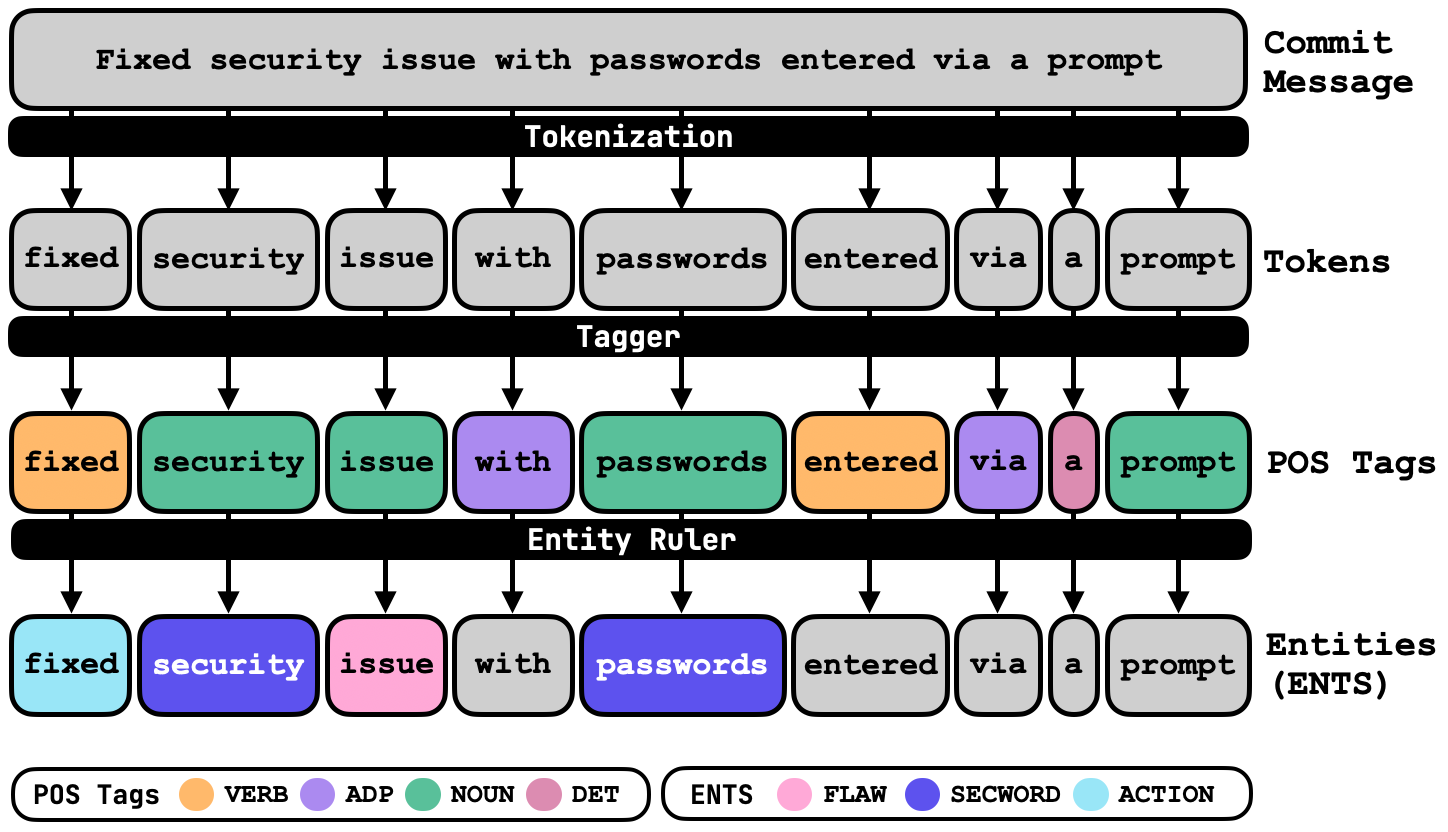
\includegraphics[scale=0.36]{Figures/parsing.png}
    \caption{Extraction Pipeline}\label{fig:parsing}
\end{figure}


\subsubsection{Rules} Fixing security vulnerabilities 
usually involves an ``ACTION'' (one of our category entities, Table~\ref{tab:entities}). Actions can be represented in natural language with verbs such as ``fix'', ``update'', ``patch'', ``mitigate'' and more. Therefore, we created several rules that search for different verbal forms of these words. 
Table~\ref{tab:rules} shows two examples of rules used by our entity ruler. The first rule extracts all the different verbal forms of the word ``fix'' (e.g., ``fix'', ``fixing'', ``fixed'', ``fixes''), i.e., it extracts all variations of the token ``fix'' when its POS tag is a \texttt{VERB}. 

\begin{table}[t!]
\footnotesize
    \centering
        \caption{NER Rule examples. All rules are 
        available in our replication package 
        (\texttt{entity\_ruler/patterns.jsonl}).} 
    \begin{tabular}{ | p{0.25cm} | p{1.25cm} | p{6cm} | }
    \hline
        \textbf{ID} & \textbf{Label} & \textbf{Rule}\\\hline
        R1 & ACTION & \verb|{"label":"ACTION","pattern":[{"LOWER": |\\& & \verb| {"REGEX":"fix.*"},"POS":"VERB"}]}|  \\\hline
        R2 &  VULNID & \verb|{"label":"VULNID","pattern":[{"LOWER":|\\& & \verb|"osv"},{"IS_PUNCT":true,"OP":"?"},|\\& & \verb|{"LOWER":{"REGEX":"\\d{4}"}},|\\& & \verb|{"IS_PUNCT":true,"OP":"?"},|\\& & \verb|{"LIKE_NUM":true}],"id":"OSV"}| 
        \\\hline
    \end{tabular}
    \label{tab:rules}
\end{table}

The second example
illustrates the extraction of different vulnerability IDs. With the 
growth of the open-source security community, different 
ecosystems (e.g., PyPI, NPM, Ruby Gems, and more) are 
starting to report vulnerabilities with their own IDs that 
follow different structures than the usual CVE ID, \verb|CVE-\d-\d{4,7}|. Therefore, we implemented rules to extract the 
different vulnerability IDs (VULNID). One example is R2, 
a rule to extract vulnerability IDs of type (or rule id) OSV for vulnerabilities 
detected with Google's OSS-Fuzzer (e.g., OSV-2023-
27\footnote{https://osv.dev/vulnerability/OSV-2023-27}). 

In  addition, we created a total of $1719$
rules---from words or 
bags of words collected in previous 
work~\cite{10.1145/3133956.3134072,10.1145/3475716.3475781}.  These rules extract security-related words (\texttt{SECWORD}). Many rules were improved after manual 
inspection of commit messages, where (1) we detected erroneous 
extraction when looking at the entities (e.g., due to broken 
tokenization of GitHub Advisory IDs, we had to create several 
different rules based on different tokenization results); or, 
(2) the tool did not extract any entity. This process led us to 
augment the list of category entities and find a set of 
anti-patterns for security commit messages---which is described in detail on Table~\ref{tab:fields}. 


\subsection{Best Practices Analysis (RQ2)}

One way to produce quality 
commit messages is by following best practices or guidelines~\cite{Tian_2022, convcom,linus,atomic}. 
In this part of the study, we explored if some of the available guidelines or standards 
were already under usage and how they could be leveraged to create more structured and complete commit messages for security patches.
We found six main suggestions to produce good commit messages from four sources of guidelines~\cite{convcom,goodcommit,linus,Tian_2022}: (1) conventional commits suggest adding a type as a prefix to the subject/header such as \texttt{fix:} or  \texttt{feat:}~\cite{convcom}; (2) the header should explain the commit in one line and meaningful~\cite{convcom,goodcommit} in the capitalized form, no period in the end and the imperative form~\cite{goodcommit}; (3) the body should explain the problem (what), its impact (why) and the fix (how)~\cite{linus,Tian_2022}; (4) the message should include references to bug-trackers, issues or pull requests (when GitHub is used to manage defects)~\cite{goodcommit}; (5) contacts of the reviewers and reporters~\cite{linus}; and finally, (6) keep commits atomic, i.e., one task per commit~\cite{goodcommit}.

We translated the suggestions mentioned before into seven different compliance checkers, which we used to assess if security engineers are following best practices. Table~\ref{tab:practices} shows the different compliance checkers and their sources. %



\begin{table}[t!]
    \footnotesize
    \centering
        \caption{Best Practices to Write Generic Commit Messages} 

    \begin{tabular}{| p{0.25cm} | p{6cm} | p{1.25cm} | }
    \hline
        \textbf{ID} & \textbf{Best Practice} &  \textbf{Standard}
        \\\hline
        C1 &  The header should be prefixed with a type.  & ~\cite{convcom} \\\hline
        C2 & The message should have a one-line header/subject.  & ~\cite{convcom, linus, goodcommit}\\\hline
        
C3 & The message should have a body.  & ~\cite{linus, goodcommit}\\\hline

C4 & The message should mention the contact of the author (signed-off-by and authored-by).  & ~\cite{linus, goodcommit}\\\hline

C5 & The message should mention the contact of the reviewer (reviewed-by).  & ~\cite{linus, goodcommit}\\\hline

C6 & The message should mention references to issues or pull requests.  & ~\cite{goodcommit}\\\hline

C7 & The message should include references to bug trackers.  & ~\cite{goodcommit}\\\hline

    \end{tabular}
    \label{tab:practices}
\end{table}

\section{SECOM: A Convention for Security Commit Messages and its Validation}~\label{sec:solution}

To address the problems mentioned in the previous section, we propose SECOM, a convention for writing security commit messages; and, validate
its usage with the security 
community. The new convention helps us answer the research question RQ3.  


\subsection{Design of the Convention}

In our empirical study, we observed that although security commit messages do not follow best practices in general, there is a small percentage of people using them---i.e., best practices are being used by some security engineers even if only by a small percentage (Section~\ref{sec:findings}). To facilitate adoption, we created \texttt{SECOM} on top of a well-known group of 
guidelines
for writing good commit messages~\cite{convcom, atomic, linus, goodcommit}.  
Table~\ref{tab:fields} lists and describes the different fields and the reason why each field was considered (\textit{rationale}). For instance, the ``type'' field 
was considered because, according to the Conventional Commits Specification, the header/subject should start with a type ($4.10\%$ of security commit messages include a type at the beginning of the header). In addition, the Google OSV team suggested that type should be indeed considered and proposed a new word for security patches, ``vuln-fix''.

The structure and set of fields 
included in the convention were inferred 
from (1) our empirical analysis  of security
commit messages collected from security patches available in vulnerability
databases such as NVD and OSV; 
(2) feedback collected alongside
the Open Source Security Foundation community; and, (3) previous work on best practices for commit messages~\cite{convcom, atomic, linus, goodcommit,Tian_2022}.

The convention (Listing~\ref{lst:SECOM}) consists of five main 
sections: \textbf{header}, prefixed with the type \texttt{vuln-fix}, 
a simple description of the vulnerability and its identifier 
(when available); \textbf{body}, describes the vulnerability 
(what), its impact (why) and the patch to fix the vulnerability 
(how); \textbf{metadata}, such as type of weakness (CWE-ID), 
severity, CVSS, detection methods, report link, and version 
of the software where the vulnerability was introduced; 
\textbf{contacts}, the names and e-mail contacts of 
the \textbf{reporters} and \textbf{reviewers}; and, finally,
\textbf{references} to bug trackers. The different
sections should be separated with a new line.

\begin{lstlisting}[caption={SECOM Convention},label={lst:SECOM},frame=tlrb]
<type>: <header/subject> (<Vuln-ID>)

<body>
# (what) describe the vulnerability
# (why) describe its impact
# (how) describe the patch/fix

[For Each Weakness in Weaknesses:]
Weakness: <Weakness Name or CWE-ID>
Severity: <Low, Medium, High, Critical>
CVSS: <Severity Numerical Repr. (0-10)>
Detection: <Detection Method>
Report: <Report Link>
Introduced in: <Commit Hash>
[End]

Reported-by: <Name> (<Contact>)
Reviewed-by: <Name> (<Contact>)
Co-authored-by: <Name> (<Contact>)
Signed-off-by: <Name> (<Contact>)

Bug-tracker: <Bug-tracker Link>
OR
Resolves: <Issue/PR No.>
See also: <Issue/PR No.>
\end{lstlisting}

The convention considers security patches should be atomic~\cite{atomic}, i.e., two weaknesses can be patched by the same fix, but if it requires more than one fix, then it should be a different commit. 


\begin{table*}
    \footnotesize
    \centering
    \begin{tabular}{ | p{1.75cm} | p{4cm} | p{11cm} | } 
    \hline
        \textbf{Field} & \textbf{Description} & \textbf{Rationale}\\\hline
        type & Usage of \texttt{vuln-fix} at the beginning of the header/subject to specify the fix is related to a vulnerability. & A \textbf{type} should be assigned to each commit~\cite{convcom}---which will make the identification of vulnerability fixes easier. The \texttt{vuln-fix} value was proposed by the Google OSV team during the feedback collection \textbf{(F)} phase. In addition, 4.10\% of commits follow the
conventional commits convention “<type>(scope):”. \\\hline
        Header/Subject & It should be approximately 50 chars (max 72 chars), capitalized with no period in the end and in the imperative form. & According to the common best practices for commit messages, it is important to summarize the purpose of the commit in one line~\cite{linus, goodcommit}. In our best practices analysis, we observed that $100\%$ of commit messages had a header, but only $38.85\%$ had security-related words and represented an action. \\\hline
        Vuln-ID & When available, e.g., CVE, OSV, GHSA, and other formats. & Adding the vulnerability ID to the header/subject can help to localize the commit responsible for patching the vulnerability faster using features like reflog or shortlog. Only 12.1\% of commit messages included mentions of the vulnerability ID, but 4 out of the 7 participants in \textbf{(F)} phase found including the vulnerability ID in the message important.\\\hline
        Body &  Describe the vulnerability (what), its impact (why), and the patch
    to fix the vulnerability (how) in approximately 75 words (25 words per point). & The body is the most important part of the commit message since it provides space to add details on the problem, impact, and solution~\cite{Tian_2022}. In our empirical analysis, we observed that  59.91\%
    commit messages have a body. However,  only 4031 out of those 6875 cases included security-related words or had meaningful information. \\\hline
        Weakness &  Common Weakness Enumeration ID or name. & The weakness ID provides information on which type of vulnerability can exist in the software. Software patch management teams may proceed differently according to the type of weakness. However, only 0.2\% of messages included this type of information. \\\hline
        Severity &  Severity of the issue (Low, Medium, High, Critical). & Severity can motivate software users to perform patch management faster (in case of critical vulnerabilities)~\cite{Householder2020}. Again, only 1.1\% of commit messages mentioned severity levels. \\\hline
        CVSS &  Numerical (0-10) representation of the severity of a security 
    vulnerability (Common Vulnerability Scoring System). & CVSS allows users to make better sense of the vulnerability severity and can motivate software users to perform patch management faster~\cite{Householder2020}. This field was proposed by a security engineer at OpenSSF that mentioned that sometimes is possible to calculate the score by following the CVSS questionnaire. \\\hline
        Detection &  Detection method (Tool, Manual, etc). & It can be interesting to help future researchers with replication. $4$ out of the $7$ participants in the \textbf{(F)} phase sees value in adding this field (Table~\ref{tab:survey}, RQ2). \\\hline
        Report & Link for vulnerability report, which can back up the lack of information provided in commit messages. & It usually provides more information on the vulnerability exploit or proof-of-concept. We observed that 3 out of the 7 participants would like to see links to reports, \textbf{(F)} phase (RQ1). \\\hline
        Introduced in & Commit hash from the commit that introduced the 
    vulnerability. & Suggested by a survey participant of the (\textbf{F}) phase and used in the OSV Schema~\cite{osv-schema}. In addition, we found SHA keys in 1467 commit messages.\\\hline
        Signed-off by & Name and contact of the person that reported the issue.  & To provide credit to the person that found the problem and ask for more details when necessary. However, only 8.4\% of commit messages were signed off by the respective authors.\\\hline
        Reviewed-by & Name and contact of the person that reviewed and closed the issue. & Reviewers are usually the internal developers or senior developers that review and approve the issues. Only 3.33\% of messages have the reviewers' contact.\\\hline
         Bug-tracker & Link to the issue in an external bug-tracker or \texttt{Resolves... See also:} when GitHub is used to manage issues. & Important to document and discuss the problem, its impact and know which people were involved. In our empirical analysis, we extracted URLs from a total of $929$ commits. \\  
    \hline
    \end{tabular}
    \caption{Fields description and rationale.}
    \label{tab:fields}
\end{table*}

% \textbf{Threats to Validity.} Our sample of participants is small, which may not reflect the entire population. In addition, we only considered participants from the open-source community (i.e., private software developers may not be represented). 

% \textbf{Initial Impact.} SECOM was mentioned as one of 
% the best practices for bulk generation of pull requests 
% to scale vulnerability patching in conferences such as BackHat and Defcon~\cite{blackhat}.


\subsection{Compliance Checklist}

Table~\ref{tab:checklist} provides a checklist (or set of rules) to produce better security commit messages.
For each section of the convention, practitioners will find the fields that should be added to the 
security commit message and questions they should ask when filling them out. We find all the fields important; however, for the sake of prioritization when time is short, we selected some of them as mandatory---which are the ones we think to be most important to detect (type, Vuln-ID), prioritize (Weakness, Severity, CVSS) and understand the message (header, what, why, how). However, practitioners should always try to make security commit messages as detailed as possible. The compliance validation with \texttt{SECOM}'s structure (Listing~\ref{lst:SECOM}) and rules (Table~\ref{tab:checklist}) is currently automated with a tool. In the future, we plan to explore how to generate suggestions to produce better security commit messages or even entire ones to soften the burden of a new standard in maintenance teams.



\begin{table*}
    \footnotesize

    \begin{tabular}{ | p{1.75cm} | p{1.75cm} | p{11.75cm} | p{0.25cm} | } 
    \hline
        \multirow{4}{*}{\textbf{Header}} & type & Did you set the type of the commit as "vuln-fix" at the beginning of the header? & \textbf{M} \\\cline{2-4}
                                & header/subject & Did you summarize the patch changes? & \textbf{M} \\\cline{2-4}
                                & header/subject & Did you summarize the patch changes within $\sim$50 chars?	 & \textbf{O} \\\cline{2-4}
                                & Vuln-ID & Is there a vulnerability ID available? Did you include it between parentheses at the end of the header? & \textbf{M} \\
    \hline\hline
        \multirow{4}{*}{\textbf{Body}} & what & Did you describe the vulnerability or problem in the first sentence of the body?	 & \textbf{M} \\\cline{2-4}
                                & why & Did you describe the impact of the vulnerability in the second sentence of the body?	 & \textbf{M} \\\cline{2-4}
                                & how & Did you describe how the vulnerability was fixed in the third sentence?		 & \textbf{M} \\\cline{2-4}
                                & * & Did you describe the what, why, and how within $\sim$75 words ($\sim$25 words per section)? & \textbf{O} \\
    \hline\hline
        \multirow{6}{*}{\textbf{Metadata}} & Weakness & Can this vulnerability be classified with a type? If so, add it to the metadata section. & \textbf{M} \\\cline{2-4}
                                & Severity & Can infer severity (Low, Medium, High, Critical) for this vulnerability? If so, add it to the metadata section.	 & \textbf{M} \\\cline{2-4}
                                & CVSS & Can you calculate the numerical representation of the severity through the Common Vulnerability Scoring System calculator (https://www.first.org/cvss/calculator/3.0)?			 & \textbf{M} \\\cline{2-4}
                                & Detection & How did you find this vulnerability? (e.g., Tool, Manual, etc) & \textbf{O} \\\cline{2-4}
                                & Report & Is there a link for the vulnerability report available? If so, include it. & \textbf{O} \\\cline{2-4}
                                & Introduced in	 & Include the commit hash from the commit where the vulnerability was introduced. & \textbf{O} \\
    \hline\hline
        \multirow{2}{*}{\textbf{Contacts}} & Reviewed-by & Include the name and/or contact of the person that reviewed and accepted the patch.  & \textbf{O}\\\cline{2-4}
                                    & Signed-off-by	 & Include the name and/or contact of the person that authored the patch.	  & \textbf{M}\\
    \hline\hline
        \multirow{2}{*}{\textbf{Bug-Tracker}} & External & Include the link to the issues or pull requests in the external bug-tracker. & \textbf{O}\\\cline{2-4}
                                    & GitHub	 & Include the links for the issues and pull-requests related to the patch (\texttt{Resolves.. See also:}).	  & \textbf{O}\\
    \hline
    \end{tabular}
    \caption{SECOM Compliance Checklist. [\textbf{M}-Mandatory; \textbf{O}-Optional; \textbf{*}-All fields in the section.]}
    \label{tab:checklist}
\end{table*}

\subsection{SECOM's Application Example}

\texttt{SECOM} is meant to structure and help write more informative and meaningful
security commit messages. In this section, we show an application example of \texttt{SECOM}
to improve the commit message used to document the patch to CVE-2012-0036\footnote{https://nvd.nist.gov/vuln/detail/CVE-2012-0036}, a potential data injection via a crafted URL.

\begin{lstlisting}[caption={Original commit message to fix CVE-2012-0036},label={lst:before},basicstyle=\scriptsize,frame=tlrb]
URL sanitize: reject URLs containing bad data
Protocols (IMAP, POP3 and SMTP) that use the path 
part of a URL in a decoded manner now use the new 
Curl_urldecode() function to reject URLs with 
embedded control codes (anything that is or 
decodes to a byte value less than 32).

URLs containing such codes could easily otherwise 
be used to do harm and allow users to do 
unintended actions with otherwise innocent tools 
and applications. Like for example using a URL 
like pop3://pop3.example.com/1%0d%0aDELE%201 
when the app wants a URL to get a mail and 
instead this would delete one.

This flaw is considered a security 
vulnerability: CVE-2012-0036

Security advisory at: 
http://curl.haxx.se/docs/adv_20120124.html

Reported by: Dan Fandrich
\end{lstlisting}

\begin{lstlisting}[caption={Commit message to fix CVE-2012-0036 (after SECOM's application)},label={lst:after},basicstyle=\scriptsize,frame=tlrb]
vuln-fix: Sanitize URLs to reject malicious data 
(CVE-2012-0036)

Protocols (IMAP, POP3 and SMTP) that use the path 
part of a URL in a decoded manner now use the new 
Curl_urldecode() function to reject URLs with 
embedded control codes (anything that is or 
decodes to a byte value less than 32).
URLs containing such codes could easily otherwise 
be used to do harm and allow users to do 
unintended actions with otherwise innocent tools 
and applications.
Like for example using a URL like 
pop3://pop3.example.com/1%0d%0aDELE%201 when the 
app wants a URL to get a mail and instead this 
would delete one.

Weakness: CWE-89
Severity: High
Detection: Manual
Report: https://curl.se/docs/CVE-2012-0036.html

Reported-by: Dan Fandrich
Signed-off-by: Daniel Stenberg (daniel@haxx.se)

Resolves: #17940
See also: #17937
\end{lstlisting}

Listing~\ref{lst:before} shows the original commit message used to document the code changes
to patch the CVE-2012-0036. Listing~\ref{lst:after} shows an example of the same commit message, 
but if the message had followed the SECOM standard convention and rules. As seen, the header
includes a type, a short message, and the vulnerability ID, followed by the body where a description
of the problem and fix is provided, and later all the information regarding metadata, contacts, and bug trackers are also provided. In the original message, details such as weakness and severity were not provided, which would not allow triage systems to prioritize this patch properly.

\subsection{Standard Validation (RQ3)}

This section describes how we collected feedback (F) from the security community about the proposed convention (SECOM). We prepared a small survey to collect feedback from the open-source security community. 

The survey did not collect any personal data, and we informed that to our participants at the beginning of the form. \texttt{SECOM} was presented and discussed in detail in two working groups of the Open-Source Security Foundation (OpenSSF). 
OpenSSF is an open community where 
security engineers from all over the industry are involved (e.g., Google, Linux Foundation, Intel, RedHat, and more) and on a mission to 
make open-source security better~\cite{OPENSSF-MISSION}. The convention was validated by experienced security engineers involved in the best practices and vulnerability disclosure projects.
At the end
of our discussion, we asked the present security engineers
to provide their feedback on the convention by answering a few questions (see
Table~\ref{tab:survey}). These questions were designed to validate the different fields
we proposed (Q1 and Q2) and to understand the community's opinion on our new solution (Q3-Q5).
For instance, we wanted to understand which field the community finds more important. One 
thing we observed in our manual analysis of commit messages was the mention of the 
process of detection of the vulnerability---sometimes, the tool used to detect the 
vulnerability was mentioned in the message. Since we did not have any strong 
data analysis to backup this decision, we asked the potential users what they 
thought about it.

\begin{table}[!b]
    \footnotesize
    \centering
    \begin{tabular}{ | p{0.25cm} | p{4.5cm} | p{1.75cm} | } 
    \hline
        \textbf{No.} & \textbf{Question} & \textbf{Answer}\\\hline
       Q1 & ``The following pieces of information commonly appear in commit messages of security-related patches.  Which do you find important to include in a security commit message?''  & Vuln-ID, Severity, CVSS, Weakness Type, Report Link\\\hline
        Q2 & ``Security vulnerabilities are usually detected by different means (e.g., manually, static analysis, dynamic analysis, penetration testing, etc.). Do you see value in reporting this information in a security commit message?'' & Yes, No, Unsure\\\hline
        Q3 & ``Would you use this or a similar convention as standard practice in your own work or advocate its use in your team?'' & Yes, No, Unsure\\\hline
        Q4 & ``If you answered "Other" or "Unsure to any of the questions, please explain briefly below.'' & Open \\\hline
        Q5 & ``Please enter any other comments or suggestions below.'' & Open \\
    \hline
    \end{tabular}
    \caption{Survey questions used to validate SECOM.}
    \label{tab:survey}
\end{table}


\section{Findings}~\label{sec:findings}

In this section, we present the main conclusions 
of our empirical analysis of security commit messages 
and the validation of \texttt{SECOM}. 

\subsection*{\textit{RQ1: What information is included in
the commit messages of public security patches?}}


We ran our extraction pipeline (Figure~\ref{fig:parsing}) over a total of $11036$ security commit messages. Table~\ref{tab:entities} shows the number of entities extracted per entity category (\#Entities), the number of commits where entities of each type were found (\#Commits), and the respective percentage of commits (\%Commits). We divided the 
entities into two main sets: security-specific and commit-specific. The tool was able 
to extract key information for both types:
$38.5\%$ of the extracted entities are security-specific, and the remaining $61.5\%$ are commit-specific.

\begin{table}[t!]
\footnotesize
    \centering
        \caption{Extraction Results} 
    \begin{tabular}{| p{2cm} | p{1.25cm} | p{1.5cm} | p{1.5cm} | }
    \hline
        \textbf{Category} & \textbf{\#Entities} & \textbf{\#Commits} & \textbf{\%Commits} \\\hline
SECWORD & 16126 & 6749 & 61.2\%\\\hline
ACTION & 10364 & 6409 & 58.1\%\\\hline
EMAIL & 4738 & 2086 & 18.9\%\\\hline
SHA & 4943 & 1467 & 13.3\%\\\hline
FLAW & 4402 & 2843 & 25.8\%\\\hline
ISSUE & 3561 & 2805 & 25.4\%\\\hline
URL & 1175 & 929 & 8.4\%\\\hline
VULNID & 1799 & 1330 & 12.1\%\\\hline
VERSION & 658 & 571 & 5.2\%\\\hline
DETECTION & 629 & 374 & 3.4\%\\\hline
SEVERITY & 142 & 118 & 1.1\%\\\hline
CWEID & 25 & 23 & 0.2\%\\\hline\hline
\textbf{Total} & 48562 & 10168 & 92.1\%\\\hline
\end{tabular}
    \label{tab:entities}
\end{table}

\textbf{Commit-specific data (COM).} The tool extracted entities for all the $7$ different entity categories classified as commit-specific. A total of $29841$ entities were extracted as commit-specific information. 
A commit usually implies an \emph{action} or \emph{change}. In the case of security, it should imply fixing a vulnerability (corrective maintenance). Yet, only $10364$ entities for verbs (ACTION) were extracted from $6409$ ($58.1\%$) commit messages. Fixing a vulnerability also means fixing a flaw. Our tool extracted mentions of flaws (FLAW) in $2843$ ($25.8\%$) commit messages. 
Mentions of issues (ISSUE) and URLs (URL) can be a good source of external documentation and information, but security engineers rarely mention that information in their commit messages: only $2805$ contained references to issues, and $929$ commit messages contained URLs. 

% Previous work showed that only $38\%$ of security commit messages included security-relevant words~\cite{9678720}. 
\textbf{Security-specific data (SEC).} The tool extracted entities for all the $5$ different entity categories classified as commit-specific. A total of $16126$ security-related words (\texttt{SECWORD}) was collected from $6749$ out of $11036$ ($61.2\%$) commit messages.
Vulnerability IDs (VULNID) were only extracted for $1330$ commit messages, while all patches that integrate our dataset, fix a vulnerability with a known ID. Vulnerability IDs easily map security commits to official reports, which usually provide more details on the vulnerability, product affected, severity, and more. Therefore, they are important to add to commit messages.
It seems that security engineers rarely mention weakness IDs (CWEID)---only $25$ entities were extracted from $23$ commits messages. We suspect that we can often extract the weakness type by looking at the set of entities extracted for the SECWORD category. For instance, in ``fixed xss vulnerability bug by oncellhtmldata'' (commit message from security patch to the GHSA-hf4q-52x6-4p57 vulnerability), we could infer a CWE-79 based on the ``xss'' entity extracted in this message. Severity can be important for security patch management systems to know which security patches to prioritize. If a patch to a critical vulnerability is released, it should be installed as soon as possible. 
However, severity entities (SEVERITY) are rarely included in security commit messages---only extracted from $118$ ($1.1\%$) security commit messages.


\textbf{Finding 1.} Security engineers
use security-related words in
$61.2\%$ of the security commit messages
used to patch software vulnerabilities.



\textbf{Finding 2.} Vulnerability IDs, Weakness IDs and Severity are rarely mentioned 
in security commit messages---although important for manual and automated detection and prioritization. 

Our tool extracted
a total of $48562$ entities from $10168$ out of the $11036$ ($92.1\%$) security commit messages under analysis. For the remaining $868$ of the commit messages, we performed a manual validation of the reason behind of null extraction:
%(Table~\ref{tab:reasons}):

\textbf{Poorly-Written.} We found several types of poorly-written messages reported in previous work~\cite{Tian_2022}. For instance, we found $51$ messages containing only one token (``Single-word''). Some examples are ``update'', ``...'', ``:arrow\_up:'', ``Refactor''. Poorly-written messages usually contain one line without clear information regarding the commit’s purpose (e.g., ``applied updates'', ``backend media''. We found a total of $760$ messages that lacked meaningful information. 

\textbf{Non-Security Related.} Dense message with no clear relationship with security. One example is 
``Support progressive event for dc. This implements the progressive api event fo rthe dc image. This is currently only supported for vardct without extra channels: for
modular and extra channels it's only supported if squeeze is used, and
it may not correctly work with flush yet in that case.''---the commit message of OSV-2021-1606 vulnerability.
We found a total of $97$ commit messages that were hard to relate with security fixes. 

\textbf{Misspelling Issues.} Messages with misspelled english words that would be detected if well written. One example is the message: ``sanitzing user input ''.
However, this kind of issues reflects a very small percentage of the problem.



% \begin{table}[t!]
%     \centering
%         \caption{Reasons why the NER tool failed extraction} 
%     \begin{tabular}{| p{3cm} | p{4cm} | p{0.5cm} | }
%     \hline
%         \textbf{Pattern} & \textbf{Description} &  \textbf{No.}
%         \\\hline
%         Poorly Written  & Containing usually one line without clear information regarding the commit's purpose.   & 760 \\\hline
%         Non-Security Related  & Dense message with no relationship detected with security.  & 97 \\\hline
%         Misspelling Issues & Misspelled english words that lead to unsuccessful extraction. & 11 \\\hline
%         Total &  & 868 \\\hline
%     \end{tabular}
%     \label{tab:reasons}
% \end{table}

\textbf{Finding 3.} No extraction of entities was performed from $8\%$ of security commit messages mainly due to poorly written messages, misspelling issues and no clear connection with security.


\subsection*{\textit{RQ2.  Do security engineers follow best practices to write security commit
messages?}}

We applied $7$ compliance checkers to the commit messages to evaluate if security engineers are using generic best practices to write commit messages since no standard for security exists.

\textbf{C1.} One way of easily marking a commit message for an automated solution is with the usage of a prefix in the header (as the Conventional Commit Convention proposes~\cite{convcom}). In security, this practice was only used in 453 out of 11036 (4.10\%) of commits follow the conventional commits convention ``<type>(scope):'' using prefixes such as ``patch'' or ``fix''.

\textbf{C2.} Headers are important because they are ultimately used to make a quick searches of relevant commits through the git reflog feature. Therefore, it is important that all commit messages have a meaningful and clear header. All the security commit messages (100.00\%) have a one line subject/header. But only 4288 out of 11036 (38.85\%) headers have security-related words (SECWORD) and reflect an action (ACTION).

\textbf{C3.} Previous work has shown that a good commit message needs to clearly mention the problem (what), its impact (why) and how it will be fixed (how)~\cite{Tian_2022}. However, only 6875 out of 11475 (59.91\%) commit messages have a body. Security engineers do not use often security related-words (or vocab) in their body messages since only 4031 out of 11036 (36.53\%) of body messages have SECWORDS.

\textbf{C4.} Crediting the authors of the fixes by signing-off by commits is a very well known practice in security. However, only 925 out of 11036 (8.4\%) commit messages were signed-off by the authors.

\textbf{C5.} Reviewers are usually the internal developers or seniors developers that review and approve the issues. Only 368 out of 11036 (3.33\%) of messages have the reviewers contact.

\textbf{C6.} Issues are good sources of documentation since they sometimes provide details on the discussion of the problem and potential solution. However, only 2805 out of 11036 (25.42\%) commit messages have references to issues.

\textbf{C7.} Same as references to issues, links to bug trackers are also good to mention since they usually provide useful documentation on the problem, fix, severity, and more. But again, only 196 out of 11036 (1.78\%) of commits have references to bug trackers.


\textbf{Finding 4.} Security engineers, do not follow best practices to write security commit messages in general. Even when it seems they are, we concluded that key information is missing---which indicates we need best practices for writing better security commit messages. 


\subsection*{\textit{RQ3. How open is the security community to a new standard for security commit messages?}}

Feedback received from the security community suggests that they see value in SECOM and would like to see it evolve into a standard practice---6 out of the 9 participants responded ``Yes''
to Q3 (``Would you use this or a similar convention
as standard practice in your own work or advocate its use in your team?''), the remaining three participants answered ``Unsure''. None of the participants answered ``No''. 2 out of 9 participants said they did not find valuable to mention how the vulnerability was detected. However, 6 of the 9 participants answered ``yes''. Therefore, we considered the ``Detection'' field in the convention. The vulnerability ID, CWE ID,  and severity are the fields that participants found more important to include 
in the commit message. The least important fields are the CVSS and report link.

\textbf{Finding 5.} The security community sees value in SECOM and aims to adopt it as a standard practice in the future.

The participants that were unsure of SECOM's adoption were mainly concerned with the current practices: ``Folks won't be practicing this style daily, and for drive-by contributions, git messages are likely to be highly ad hoc and idiosyncratic.''. However, we argue that with good automated tools, we can help developers produce better commit messages for security. Writing more structured and informative commit messages is important since, ultimately, it can improve the detection and assessment capabilities of patch triage systems and enable fast patch management. 











\section{Implications and Considerations}\label{sec:discussion}

In this section, we describe the implications of 
our findings, ethical considerations, and how 
SECOM should be used.

\subsection{Dealing With Patch Transparency}\label{sec:transparency}

 Transparency is a double-edged sword. It can be a source of trust for consumers~\cite{Householder2020}, but it also creates vulnerability~\cite{9678720}, and, the need for security is often used to avoid transparency because of the risks that come from it. The reality is that non-transparent processes lead to abuse and make timely patch management a challenge (or even impossible). The CERT Coordinated Vulnerability Disclosure (CVD) guide suggests avoiding silent patches since it hinders public awareness of fixes to software vulnerabilities. This, then, leads to a lack of understanding and trust from developers and to poor triage systems (automated tools are incapable of reasoning about data and detect patches if no key information is provided).
 
 The SECOM convention and best practices purposed in this paper are meant to 
help vendors to produce better documentation and boost the patch 
management phase---responsible for deploying the new changes to the users. We are aware that being too much transparent can make users vulnerable to cyberattacks, but we argue that providing better documentation will help automated tools be more effective and fast for software security patch management. So, OSS users and companies can benefit from an automated solution by being aware 
of the fixes as soon as they are developed, which is usually one week earlier than
the disclosure~\cite{10.1145/3133956.3134072}.  

Experienced security engineers should determine when and not when to provide details. If development systems are private, 
then no major risks are attached to providing a detailed security commit message (in principle, we do not account for internal attackers). However, when a critical vulnerability is to be patched in open-source software of wide use, then security engineers should carefully decide which details to include in the commit message. They should provide enough information to users understand its criticality but not enough to attackers leverage.

One thing we do not advocate is the documentation of exploits since this would clearly benefit malicious attackers. That kind of information should be released later, after providing time for the users to deploy the patch.

\subsection{The Burden of a New Standard}

Applying new best practices is usually taken as a burden by the software and security communities, but it is also how we prevent and solve current challenges. As we mentioned before, well-structured and complete documentation is crucial to create trust between different parties and faster patch management---to decrease the user's exposure window. Therefore, we, as a team, and part of the software engineering community, are working on automated solutions for compliance validation and the generation of commit messages to reduce the bottleneck that our standard could introduce. \texttt{SECOM} can also be leveraged to guide other solutions to generate commit messages~\cite{7203049}. It is also important to notice that the open-source security community sees value in SECOM and aims to adopt it as a standard practice in the future. In fact, some security researchers are already using it and considering it as standard best practice~\cite{blackhat}, and more than 2k commit messages were produced following our solution.

\subsection{Need for Better Patch Documentation}

Previous work has shown that the software patch detection problem could not be solved only with security commit messages (or other types of metadata)~\cite{DBLP:journals/corr/abs-1806-05893,9678720}---which we agree. The solution proposed is to focus on code information instead. One study proposed a mixed solution~\cite{SSPatcher2022}. However, we think that focusing on code information will not fix the issue soon due to the complexity of the patterns under analysis (software vulnerability), the approaches gaps (e.g., machine learning, deep learning~\cite{9448435}), the diversity of weaknesses and many more. Instead, we can make an extra effort to provide better documentation and not only improve automated solutions but also build trust between vendors and users---which we argue will ultimately build a safer environment.


\section{Threats to Validity}\label{sec:t2v}

This section discusses the study's potential threats to validity.

\textbf{Internal Validity:}  In the survey study, our sample of participants is small, which may not reflect the entire population. However, we ensured that all the answers come from a reliable and expert source (OpenSSF). In addition, we only considered participants from the open-source community (i.e., private software developers may not be represented).

\textbf{External Validity:} We did not check for all the rules described in the standards considered. Therefore, our conclusion may not reflect the entire ground truth. But, we did check the most important rules, the ones related to having a type, header, and body in the commit message which improves the commit messages considerably.


% This section looks pretty short. Normally needs to be divided into External Validity (generalizability, related to the diversity of the data) and Internal Validity (possible flaws in the design, methodology, data collection, measurement, representation of constructs used). The one threat that was mentioned is internal validity, related to reliability. Is this section complete, or to be completed. At least one could say "the biggest internal threat to the study is ... (the one you mentioned)", and then comment on external validity, whether the conclusions can be generalized to all security commit messages, or a subset (e.g, open-source), or even a smaller subset of OS typified by the data collected.


\section{Related Work}\label{sec:rw}

This section summarizes previous research work in the fields
of Software Security Patch Management, Software Security Patch
Detection and Commit Message Analysis.

\subsection{Software Security Patch Management}

Software security patch management is the process of identifying, acquiring,
testing, installing, and verifying security patches for software products and systems~\cite{DISSANAYAKE2022106771}. 
Security patches are considered the most effective strategy to mitigate software vulnerabilities~\cite{DISSANAYAKE2022106771,SOFT-PATCH-MANAG-NIST,10.1145/2660267.2660329}.
They are prioritized over non-security patches as they aim to protect users from cyberattacks~\cite{SOFT-PATCH-MANAG-NIST}. 
Yet, one important challenge still prevails, the \emph{lack of efficient patch triage systems} to identify and prioritize security patches~\cite{Zhang2021AnIO, SSPatcher2022,hacker-news-patches,DBLP:conf/soups/LiRMMC19}: current processes are largely manual (time-consuming) and prone to ignore important bug fixes such as the one behind Equifax~\cite{failed-to-deploy-patch}.
Figure~\ref{fig:cycle} shows part of the patch management process: \emph{1)} vendors release a patch to mitigate a vulnerability previously identified or reported; \emph{2)} automated or manual systems identify and prioritize the patch and trigger patch deployment; \emph{3)} the patch is deployed successfully into the users' machines. In this paper, we propose a solution that can improve the understanding and identification of security patches for automated and manual triage systems, which can consequently decrease the time users are exposed to vulnerabilities. 
Silent fixes, i.e., software vulnerabilities patched without any release note, hinder security patch management since they leave users unaware of the new patches and their criticality~\cite{Householder2020}---knowledge about the fix is key for successful patch deployment. 
Previous work has shown that $56.7\%$ of the security commit messages are documented poorly~\cite{10.1145/3593434.3593481}, which hinders the different triage systems tasks.
This paper presents a solution to make security commit messages more informative and enable the effectiveness of patch management processes.

\subsection{Software Security Patch Detection}

Version control systems are used to maintain a record of code changes
and manage access to codebase development artifacts~\cite{10.1145/2950290.2950364}. As with any type of code changes, security patches are pushed to codebases through commits. Each commit contains changes to source code and a message explaining what changes
are made and why~\cite{883028,Tian_2022}. Over the past years, many approaches have emerged to detect security patches through metadata (e.g., commit logs, commit metadata, and associated reports) and code changes. Here, we only
mention approaches considering commit logs (or messages).
\emph{Reis et al.} detected security patches for 16 types of weaknesses in commit messages by applying different regular expressions per each kind of weakness~\cite{reis2017secbench}.
% Researchers from the security industry 
% % (Zhou and Sharma 2017; Sabetta and Bezzi
% % 2018) (from SourceClear, Inc., and SAP, respectively)
% have presented early investigations on the prediction of security issues in relation with
% commit changes.
\emph{Zhou and Asankhaya}  leveraged regular expressions to identify
features for predicting security-relevant commits in commit logs,
commit metadata, and associated bug reports. Features are vectorized and learned by word2vec~\cite{10.1145/3106237.3117771}. 
\emph{Sabetta and Bezzi} extended previous work by considering code changes as well~\cite{DBLP:journals/corr/abs-1807-02458}---which led to considerable performance improvements.
\emph{Sawadogo et al.} proposed SSPCatcher, a co-Training-based approach to catch
security patches as part of an automatic monitoring service of code repositories~\cite{SSPatcher2022}. Detection is based on the result of two Support Vector Machine classifiers: 1) one trained with commit logs; and, 2) one trained with code features. In order to identify a new security patch, both 
classifiers have to be in agreement. In this study, we do not propose a new model or approach to detect security patches. Instead, we empirically analyze security commit messages and propose a standard that can improve the effectiveness of the different triage systems tasks (e.g., detection, assessment, and prioritization).

\subsection{Security Commit Message Analysis and Standards}

Previous work has shown that only $38\%$ of security commit messages used to ``silently'' patch software vulnerabilities in the past included security-related words~\cite{9678720}. In this work, 
we analyzed the commit messages attached to all security patches to known software vulnerabilities instead of only focusing on silent fixes. As mentioned before, we were unable 
to find a convention or standard for security commit messages. Instead, we only 
found guidelines and specifications for general commit messages. The preliminary results
of this study were published before~\cite{9796324}. This paper is an extension and 
detailed report on how we analyzed the data, the results, and the design of our solution.

\section{Conclusions and Future Work}\label{sec:fw}

In this study, we observed that security commit messages integrate some relevant information for automated and manual triage systems but not enough to map them to bug reports or know which patches to prioritize. We also observed that no standards exist for security and that security engineers usually do not follow best practices. This paper presents a solution for 
the lack of structure, and key information in the  
commit messages of security fixes. we built SECOM, a convention for security commit messages, based on our empirical analysis findings and the open-source security community feedback and approval. 

Although part of the security community worries about the attacks that potentially will come from transparency, there seems to be space in the security community for a new standard that is already helping security engineers produce better security commit messages. However, it should be used carefully and consider the software vulnerability impact and time response of the maintenance team. 
%
In the future, we plan to release automated solutions for compliance validation and message generation to reduce the burden that a new best practice can introduce in the patching and disclosure life-cycle. 

% \section{Section B}
\label{sec:sectionb}

\subsection{Subsection A}
\label{subsec:subasectionB}

The model described can also be represented as

\begin{equation}
\dot{\mathbf{x}}(t) = \mathbf{T}\mathbf{z}(y),\  \mathbf{y}(0) = \mathbf{y}_0,\  z\geq 0 \\
\label{eq:dummyeq1}
\end{equation}

\noindent where

\begin{equation}
\mathbf{A} = \left[ \begin{array}{cc} -(a_{12} + a_{10}) & a_{21} \\ a_{12} & -(a_{21} + a_{20}) \end{array} \right],\ \mathbf{x} = \left[ \begin{array}{c} x_1 \\ x_2 \end{array} \right] \\
\label{eq:dummyeq2}
\end{equation}

Also, using glossaries in the math environment, you can write
\begin{equation}
\gls{A} = \frac{\gls{mflow}\gls{_v}}{\rho u}
\label{eq:dummyeq3}
\end{equation}

Note that \gls{A} is not \gls{a}.


\subsection{Subsection B}
\label{subsec:subbsectionB}

Another example for the notation section: think about \gls{gamma}.
And \gls{gamma}\gls{_p} with a subscript.

\begin{table}[H]
	\centering
	\caption{Dummy Table.}
	\begin{tabular}{|c|c|c|c|} \hline
		\textbf{Vendor Name} 				& \textbf{Short Name}	& \textbf{Commercial Name}	& \textbf{Manufacturer}	\\ \hline \hline
		\multirow{3}{*}{Text in Multiple Row}		&	ABC				&  ABC\textreg				& ABC SA			         \\ \cline{2-4}
		 								&        DEF				&  DEF\textreg				& DEF SA				\\ \cline{2-4}
										&        GHF			&  GHF\textreg				& GHF SA				\\ \hline
		Text in Single Row					&        IJK				& IJK\textreg				& IJK SA				\\ \hline
		Frescos SA						&        LMN			& LMN\textreg				& LMN SA				\\ \hline
		Carros Lda.						&    \multicolumn{3}{|c|}{Text in Multiple Column}							\\ \hline
	\end{tabular}
	\label{tab:dummytable}
\end{table}


\cleardoublepage

% %%%%%%%%%%%%%%%%%%%%%%%%%%%%%%%%%%%%%%%%%%%%%%%%%%%%%%%%%%%%%%%%%%%%%%
% Dummy Chapter:
% %%%%%%%%%%%%%%%%%%%%%%%%%%%%%%%%%%%%%%%%%%%%%%%%%%%%%%%%%%%%%%%%%%%%%%

% %%%%%%%%%%%%%%%%%%%%%%%%%%%%%%%%%%%%%%%%%%%%%%%%%%%%%%%%%%%%%%%%%%%%%%
% The Introduction:
% %%%%%%%%%%%%%%%%%%%%%%%%%%%%%%%%%%%%%%%%%%%%%%%%%%%%%%%%%%%%%%%%%%%%%%
\fancychapter{Infrastructure-as-Code Scripts Application}
\label{cap:chapter}

\textit{This chapter studies and improves the precision and recall of IaC tools through practitioners feedback and Generative Artificial Intelligence.}

\section{Introduction}
\label{sec:intro}
\section{Leveraging Practitoners Feedback to Improve Precision}
\label{sec:intro}

Software configuration management and deployment tools like
Puppet\footnote{\url{https://puppet.com/}}, 
Ansible\footnote{\url{https://www.ansible.com/}},
and Chef\footnote{\url{https://www.chef.io/}} became 
popular amongst software development warehouses~\cite{8919181,rahman2017factors}. 
The adoption of these tools has increased with the growing 
movement to run software in cloud servers. These tools help 
infrastructure teams increase productivity by automating various 
configuration tasks (\myeg{}, server setup). 
In short, these tools describe the environment configuration in 
a set of provisioning scripts that can be versioned and 
reused. They enable configuration consistency between different 
environments and can reduce the time required to provision and 
scale the infrastructure.
The process of managing and provisioning infrastructure through 
configuration scripts is called Infrastructure-as-Code (\iac). 
\iac\ tools take a script as input and create an infrastructure 
that typically runs in a virtual environment as output.

%
As with any piece of code, IaC scripts are also prone to defects 
such as security vulnerabilities~\cite{8812041}. For example, 
in $2020$, Palo Alto Network researchers reported the discovery 
of over $199$K vulnerable IaC templates~\cite{paloalto-unit42}. 
Specifically, $42\%$ of AWS CloudFormation templates, $22\%$ of 
Terraform templates, and $9\%$ of Google Kubernetes YAML files 
were vulnerable. In addition, researchers found more than $67$k 
\textit{potential} security smells in \iac\ scripts implemented 
in Ansible, Chef, and Puppet~\cite{9388795} through an ad-hoc 
tool created to show the presence of a new set of anti-patterns 
for security in the \iac{} domain. 
These reports highlight the importance of tools to prevent 
vulnerabilities from reaching production and shift security left 
in the development pipeline. 

%
Figure~\ref{lst:manifest-example} shows an example of an
\textit{Admin by default} weakness (CWE-250\footnote{CWE-250 details
available at \url{https://cwe.mitre.org/data/definitions/250.html}}),
a potential vulnerability in a Puppet manifest in a module of the
\texttt{PuppetLabs}.\footnote{Admin by default example available at 
\url{https://github.com/puppetlabs/puppet\_operational\_dashboards/blob/9eb67a407aa44c2f924f67f207edc7032f81f86a/manifests/profile/dashboards.pp\#L137} (Accessed \today)}
The vulnerability manifests when the developer
configures a user as ``admin'' or ``root'' for an
infrastructure component. In this example, the \texttt{\$grafana\_user}
is set as ``admin'' for the different services (Puppetserver, Puppetdb, Postgresql, Filesync) used by Grafana\footnote{Grafana is an open-source software
application for data exploration and visualization.
More information available at \url{https://grafana.com/}}. Therefore, 
any service can be prone to a privilege escalation attack.
In \iac{}, all the infrastructure components
are configured through scripts, including the access credentials.
Specifying default users as administrative gives privileges to users
that only an administrator should have. Admin accounts can be exploited 
to access sensitive data and execute unauthorized
code/commands. Infrastructure engineers should avoid setting admin
passwords and usernames to user accounts that do not need the privileges.
Detecting these issues automatically essential to 
make infrastructure engineers aware of possible security problems and
to help companies build more robust infrastructures.


\begin{figure}[t!]
  \centering
  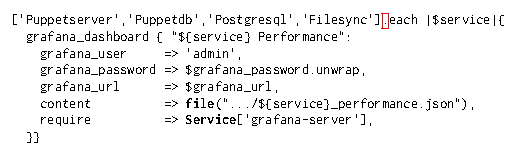
\includegraphics[width=\linewidth]{Figures/Figure-1.pdf}
  \caption{Simplified example of an \textit{Admin by default}.}\label{lst:manifest-example}
  \vspace{-3ex}
\end{figure}


\vspace{1ex}\noindent\textbf{Problem: Puppet IaC Security Linters are not reliable yet!}~In $2019$, Rahman~\etal{}
showed that \iac\ scripts---just like any piece of code---are not immune to security
vulnerabilities~\cite{8812041,10.1145/3408897}. They focused on Puppet configuration files and listed seven
anti-patterns that could lead to security vulnerabilities. The work led to the development of \slic,
a linter to detect those defects in Puppet scripts. Linters are often
imprecise tools~\cite{6606613,7781843,10.1145/1646353.1646374,8622456,8530713,46576}.
Therefore, motivated by the report of very high accuracy (i.e., precision and recall)
from their paper (Table IV~\cite{8812041}), we
decided to conduct a reproduction study of \slic{} based on a
different and larger set of projects. We asked students (co-authors of
this paper) and developers to analyze the warnings that the tool reports.
To validate the students observations of low precision, we reported a sample of the
warnings of the tool to maintainers of \botTotalRepos\ open-source projects. From
the \botTotalIssues\ issues created, we obtained responses to
\botTotalIssuesAnswers\ issues where only \botFinalIssues\ issues were discussed or clear. 
Results showed that the tool performs differently in a new 
set of projects, particularly when validated by the software owners. 
The precision observed was 
smaller than the one reported in SLIC's original 
paper (\botPrecision\ instead of $99\%$)
which indicates that security IaC linters for Puppet
are not reliable yet due to the high false positive rates.

Like many linters, \slic\ uses simple rules to detect issues.
Essentially, it searches for string patterns in
the values of tokens (many times) regardless of their 
type (e.g., variable, string, etc.)
and the relationship between them. For instance, the
``Usage of Crypto. Algorithms'' checker  
(CWE-326\footnote{CWE-326 details are available at \url{https://cwe.mitre.org/data/definitions/326.html}})
searches for any token whose value includes \texttt{sha1} or \texttt{md5}.
Both are built-in Puppet functions and \slic{} fails to consider
the context of usage of these algorithms, i.e.,
these functions are called in Puppet manifests to
encrypt data (e.g., \CodeIn{$encrypt\_key = md5($key)}).
Therefore, \slic{} incorrectly detects 
\CodeIn{md5checksum = '07bd73571b7028b73fc8ed19bc85226d'} as a CWE-326. 
This simplicity creates much noise for developers. In this preliminary study, 
we observed that the rules for the current IaC security anti-patterns 
must be better designed to be safely adopted by the industry and avoid 
productivity disruption.

\vspace{1ex}\noindent\textbf{Solution:}~Our preliminary study revealed
that (1) there is a need to improve the precision of IaC security linters for Puppet, 
and that (2) security tools can be iteratively improved and extended by incorporating 
feedback from the developer community as suggested in previous work~\cite{46576}. 
This paper reports on 
the process we followed to iteratively and 
incrementally improve the precision of an IaC linter according to user 
feedback. For example, the experiments described above ignited 
discussions with members of the development and security teams of 
Puppetlabs\footnote{GitHub PuppetLabs
organization website: \url{https://github.com/puppetlabs}}, as well as one
project manager from Vox Pupuli\footnote{Vox Pupuli is the organization responsible for maintaining
modules and tools for the Puppet community: \url{https://voxpupuli.org/}}.
The feedback collected from the team, OSS maintainers and the Puppet 
community led to the creation of a new tool, which we dubbed as \toolname{}.
Later, we leveraged the expertise of practitioners experienced 
in IaC tools or security to iteratively and incrementally
improve the new tool.

Figure~\ref{fig:timeline} shows the timeline of feedback collection 
followed to design and improve \toolname{}.
To sum up, we bootstrapped the design of \toolname\ with rules obtained 
from the revision of SLIC's ruleset, according to the feedback of the 
research team and owners of OSS projects (\textit{phase 1} in
Figure~\ref{fig:timeline}); and, incrementally evolved the linter
according to the recommendations of practitioners
(\textit{phase 2} in Figure~\ref{fig:timeline}). We improved
\noRulesSlic\ rules of the \slic{} ruleset and added
\newRules\ new rules that were either recommended by practitioners (e.g. weak
password); or relevant for the infrastructure domain (e.g. homograph
attacks\footnote{Apple Domain Attack (2017):
\url{https://www.xudongz.com/blog/2017/idn-phishing/}} and malicious dependencies).

\begin{figure}[t!]
  \centering
  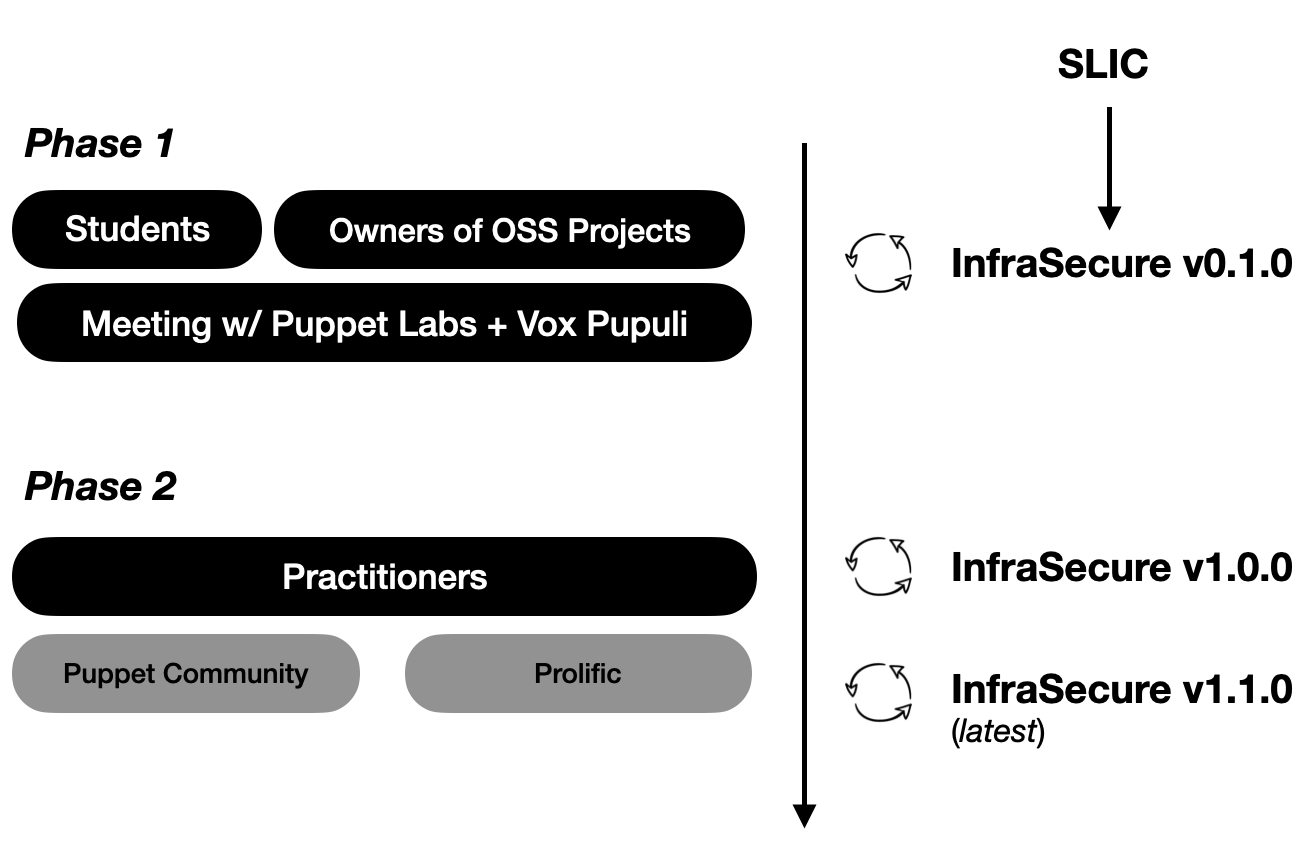
\includegraphics[width=\linewidth]{timeline.png}
  \caption{Timeline of feedback collection.}\label{fig:timeline}
  \vspace{-3ex}
\end{figure}

\vspace{1ex}\noindent\textbf{Main Results:}
This paper performs the following contributions:

\begin{itemize}[topsep=.2ex,itemsep=.2ex,leftmargin=0.8em]
    \item[\Contrib{}]\textbf{Study.}~A replication study of \texttt{SLIC}'s precision,
    including a preliminary study conducted with two researchers (co-authors of this paper)
    and a study with several \github\ scripts validated by project maintainers;
    \item[\Contrib{}]\textbf{InfraSecure.}~A new linter
    adjusting \noRulesSlic\ rules of the original
    \slic\ ruleset and adding \newRules\ new rules with a final precision of \finalPrecision.
    \item[\Contrib{}]\textbf{Dataset.}~A dataset of \iac{} scripts with more than $1000$ warnings
    classified as false positives and true positives that researchers can use to evaluate
    other security linters;
\end{itemize}

\noindent\textbf{\textit{Take-away message:}}~The takeaway message of
this paper is that it is feasible to tune security linters to produce
acceptable precision for important classes of warnings (confirming the
findings reported in a study at Google~\cite{46576}) and
that involving practitioners in discussions is an effective way to
guide the improvement of those linters.

\noindent\textbf{\textit{Replication Package:}}~All the scripts and data
    used in this study (including feedback obtained from the maintainers and practitioners)
    are available at: \repPackage{}.

	%%%%%%%%%%%%%%%%%%%%%%%%%%%%%%%%%%%%%%%%%%%%%%%%%
\section{Background}\label{sec:background}
%%%%%%%%%%%%%%%%%%%%%%%%%%%%%%%%%%%%%%%%%%%%%%%%%

This section provides background information on Puppet and
discusses security weaknesses in \iac\ scripts.

\begin{table}[!t]
  \small
  \centering
  \setlength{\tabcolsep}{3pt}
  \caption{Examples of security smells per weakness.}
  \vspace{-2ex}  
  \label{tab:examples}
  \begin{tabular}{ll}
   \toprule
   \textbf{CWE}   &  \textbf{Example} \\\midrule
   CWE-798  & \$username = ``mariadb''\\
   CWE-259  & \$password = ``!TQ23Rg''\\
   CWE-321  & \$key = ``A67ANBD7''\\
   CWE-319  & \$req = ``http://www.domain.org/secret'' \\
   CWE-546  & \#https://bugs.debian.org/cgi-bin/bugreport.cgi?bug=538392 \\
   CWE-326  & password => md5(\$debian\_password) \\
   CWE-284  & \$bind\_host = ``0.0.0.0'' \\
   CWE-258  & \$rabbitmq\_pwd = ``'' \\
   CWE-250  & \$user = ``admin'' \\
   CWE-521  & pwd => ``12345'' \\
   CWE-1007 & \$source = "http://deb.debi\mhl{a}n.org/debi\mhl{a}n" \\
   CWE-829  & \$postgresql\_version = 8.4 \\
   \bottomrule
  \end{tabular}
  \vspace{-2ex}
\end{table}

% %
\subsection{Puppet}

Developers no longer
deal with systems composed of a single machine and database.
Instead, system administrators must manage multiple diverse operating systems, databases, and virtual machines.
Perhaps most importantly, they must ensure their
configurations are consistent at any given time. Configuration management
technologies have been around for over a decade---Puppet was founded in $2005$.
Puppet is a solution that helps IT infrastructure management through 
code by supporting software deployment, packages,
and configuration. In Puppet, programs
are written using Puppet's declarative language. They are
called manifests. More information about the language can be found 
elsewhere\footnote{More about Puppet: https://puppet.com/docs/puppet/7/puppet\_overview.html}.


\subsection{Security Weaknesses}

This section describes in more detail the potential weaknesses 
in Puppet scripts. Table~\ref{tab:examples} illustrates 
examples of each weakness.

\textbf{Hard-coded secrets (CWE-798):} This warning refers to the practice of
including sensitive information such as passwords or cryptographic keys in
code files. Table~\ref{tab:examples} shows a hard-coded 
password example.
Rahman \etal{} considered $3$ kinds of data as
sensitive: usernames, passwords, and cryptographic keys. 
However,
the Common Weakness Enumeration\footnote{CWE-798 description is available at \url{https://cwe.mitre.org/data/definitions/798.html}}
list does not consider solo hard-coded usernames as a threat.
Practitioners
involved in our validation studies shared the same opinion. Therefore,
we argue that hard-coded usernames should be only reported
when there is a paired password (CWE-259) or cryptographic key (CWE-321).
More discussion on this is provided later in Section~\ref{sec:design}.


\textbf{Use of HTTP without TLS (CWE-319):} This warning refers to the practice
of using HTTP without the Transport Layer Security (TLS) to transmit
sensitive data. This means that attackers can more efficiently exploit the
communication channel as the data is transmitted unencrypted, as
cleartext\footnote{This type of issues can lead to man in the middle (MITM) attacks: \url{https://owasp.org/www-community/attacks/Man-in-the-middle_attack}}.

\textbf{Suspicious comment (CWE-546):} This warning refers to
 comments that suggest the presence of bugs, missing security functionalities,
or weaknesses of a system. Details provided in comments about bugs, security functionalities
or weaknesses can be crucial for hackers to exploit the infrastructure.

\textbf{Use of weak cryptography algorithms (CWE-326):} This warning refers to
using weak crypto algorithms.
Attackers can easily crack the encryption schemes and have
access to the data~\cite{10.1007/11426639_2}.

\textbf{Invalid IP address binding (CWE-284):} This warning refers to
assigning the address 0.0.0.0 to a server.
This practice allows connections from any IP address to access 
that server~\cite{DBLP:conf/raid/Mutaf99}.
While mail servers have to listen on 0.0.0.0 to receive
mail, database servers should not since it can lead
to critical data breaches.

\textbf{Empty password (CWE-258):} This warning refers to using
empty strings as passwords, which are easily
guessable.

\textbf{Admin by default (CWE-250):} As detailed in the Introduction, this warning refers to
defining users with administrative privileges. This can result in security
weaknesses since it can disable or bypass security checks performed by the system.\footnote{Why
you should not use an admin account: \url{https://www.lbmc.com/blog/why-you-should-not-use-an-admin-account/}}

\textbf{Weak Password (CWE-521):}
This warning refers to the usage of weak passwords. Weak passwords
are easily guessable and can be bypassed to gain access to systems.

\textbf{Insufficient Visual Distinction of Homoglyphs Presented to User (CWE-1007):}
This warning refers to malicious actors using homoglyphs
that may cause the user to misinterpret a glyph and perform an unintended, insecure action.
The homograph attack performed against the apple website\footnote{Phishing
with Unicode domains:~\url{https://www.xudongz.com/blog/2017/idn-phishing/}} is a well-known
example of this type of weakness. Table~\ref{tab:examples} shows an example of a domain where 
the character ``\mhl{a}'' could be replaced by the respective homoglyph, as in the apple attack.
This warning might be essential to uncover malicious domains implanted by malicious open-source
contributors---typosquatting attacks.\footnote{OpenSSF post on scanning OSS software for malicious behavior:~\url{https://openssf.org/blog/2022/04/28/introducing-package-analysis-scanning-open-source-packages-for-malicious-behavior/}}

\textbf{Malicious Dependencies (CWE-829):} This warning refers to malicious software
by nature, i.e., dependencies that integrate known vulnerabilities (CVEs).
These are the leading cause of supply chain attacks, and one of the main
challenges the security community faces nowadays~\cite{9402108}. 

\section{Preliminary Study}\label{sec:preliminary_study}

This section reports on the findings of two studies---involving
different sets of participants---to assess the performance of SLIC, 
a recently-developed linter for Puppet.


\subsection{Validation with Students}\label{sec:research_team}

This section reports on a study involving two of this paper's 
authors to assess the precision of \slic\ on an
independent benchmark. The study consisted in inspecting
\fpSampleSize{} warnings reported by the tool. The warnings
were validated by one senior PhD student whose research focuses 
on security and static analysis and one junior PhD student 
in software engineering with basic security skills. 

\subsubsection{Dataset}\label{subsec:dataset}

\sloppy
To build our dataset, we mined \github\ projects containing \texttt{Puppet} scripts. 
We used three different queries to search for repositories: 1) \CodeIn{language:puppet is:public}; 2) 
\CodeIn{puppet in:readme is:public}; and, 3) \CodeIn{devops is:public}. We discarded results pointing 
to forked repositories (to avoid duplicates) and discarded results pointing to repositories without 
any code in \texttt{Puppet} scripts. Our crawler found a total of \totalMinedRepos{} GitHub repositories 
and \totalMinedScripts{} associated \texttt{Puppet} scripts. \slic\ scanned these scripts for the
seven sins and reported a total of \textbf{\minedWarnings} security warnings involving 
\minedScriptsWarnings{} \texttt{Puppet} scripts (=$26.5$\% of the total) from \minedReposWarnings{} 
repositories (=$73.5$\% of the total).
Table~\ref{tab:sins_large} shows the breakdown of warnings reported by \slic. Column ``Rule'' shows the name (kind) of the warning, 
column ``\#'' shows the number of warning reports of that kind, and column ``\%'' 
shows the percentage of the total associated with that number. 
This table lists the warnings in order of their prevalence.

  \begin{table}[t]
    \small
    \centering
    \setlength{\tabcolsep}{10pt}
    \caption{\label{tab:sins_large}Breakdown of warnings reported by \slic{}.}
    \vspace{-2ex}
    \begin{tabular}{lrr}
      \toprule
      Rule & \multicolumn{1}{c}{\#} & \multicolumn{1}{c}{\%}  \\
      \midrule
      Hard-coded secrets & \hardcodedSecretsMined{} & 69.9 \\
      Use of HTTP without TLS & \httpWithoutTLSMined{} & 11.7 \\
      Suspicious comments & \suspiciousCommentsMined{} & 8.7 \\
      Use of Weak Crypto. Algos. & \weakCryptoMined{} & 4.7\\
      Invalid IP Address Binding & \emptyPassMined{} & 2.4\\
      Empty Password & \invalidIPMined{} & 2.1\\
      Admin by default & \adminDefaultMined{} & 0.5 \\
      \midrule
      Total & \minedWarnings{} & 100 \\
      \bottomrule 
    \end{tabular}
    \vspace{-2ex}    
  \end{table}


\subsubsection{Methodology}\label{sec:pre_meth} \textbf{Samples.}
Given the high number of warnings reported by the tool (\minedWarnings) and the need for 
humans to analyze each warning, we sampled a set of reported warnings. 
We leveraged two popular complementary sampling strategies to that end~\cite{strat-sampling}. 
\textit{Stratified sampling} is a method to draw samples from a set by taking into account the 
distribution of kinds---in our case, the distribution of kinds of warnings. A \textit{proportional} (stratified) sampler draws samples in a number proportional to 
the size of the sets associated with each kind whereas an \textit{uniform} (stratified) 
sampler draws the same number of samples for each kind.
% To contrast, a proportional sampler 
% draws much more warnings of the kind ``Hard-coded secrets'' compared to ``Admin by default''
% whereas an uniform sampler draws the same number of warnings for both types. 
Intuitively, 
a proportional sampler values more the most prevalent kinds of warnings (as to make more 
accurate measurements on those kinds) whereas an uniform sampler treats every kind equally 
(as to avoid inaccurate measurements on uncommon kinds).
We sampled \proportionalSampleSize{} warnings \textit{proportionally} and \uniformSampleSize{} 
(=36*7) warnings \textit{uniformly}. In total, we analyzed  
\fpSampleSize\ warnings, which is a substantial increase when compared to the 
\akondFpWarnings\ warnings analyzed in the \slic{}'s paper~\cite{10.1145/3408897}. \textbf{Metric.}
We focused on precision to measure the reliability of the reports of 
the tool. 
% Precision is the ratio between the number of true warnings 
% (True positives or TP) reported and the total number of warnings reported by a 
% given tool, including false warnings (false positives or FP). 
% \begin{align}
% 	Precision = \nicefrac{TP}{TP+FP}\label{eq:prec} 
% \end{align}
Precision is especially important for security linters. Reporting scores of false 
warnings can be highly disruptive for a team's productivity, as team members tend 
to interrupt work to address high-priority tasks~\cite{DistefanoEtAlCACM2019}. Developers 
are less willing to use linters with low rates of precision because they find them not 
trustworthy and unreliable~\cite{46576}. \textbf{Statistical Tests.} Each one of the \fpSampleSize\ warnings was 
manually inspected by two co-authors. Cases where the authors found disagreement were discussed to reach 
a consensus. We report on the results of a Cohen's Kappa
analysis~\cite{cohen1960coefficient} to measure the inter-rater 
reliability of human decisions.
%
\subsubsection{Results}

\begin{table}[t]
  \small
  \centering
  \setlength{\tabcolsep}{3.5pt}
  \caption{\label{tab:prel_analysis_slic}Performance of SLIC. (Validation with Students)}
  \vspace{-2ex}
  \begin{tabular}{lrrrrrr} 
    \toprule
    \cellcolor{Gray} \textbf{\slic{}} & \multicolumn{3}{c}{\textit{proportional}} & \multicolumn{3}{c}{\textit{uniform}} \\\midrule
    Rule & \#TP & \#FP & Pr. &  \#TP & \#FP & Pr. \\
    \midrule
    Hard-coded secrets & \tpHardcodedSecretsProportional{} & \fpHardcodedSecretsProportional{} & \precHardcodedSecretsProportional{} & \tpHardcodedSecretsUniform{} & \fpHardcodedSecretsUniform{} & \precHardcodedSecretsUniform{} \\
    Use of HTTP without TLS & \tpHttpWithoutTLSProportional{} & \fpHttpWithoutTLSProportional{} & \precHttpWithoutTLSProportional{} & \tpHttpWithoutTLSUniform{} & \fpHttpWithoutTLSUniform{} & \precHttpWithoutTLSUniform{} \\
    Suspicious comments & \tpSuspiciousCommentsProportional{} & \fpSuspiciousCommentsProportional{} & \precSuspiciousCommentsProportional{} & \tpSuspiciousCommentsUniform{} & \fpSuspiciousCommentsUniform{} & \precSuspiciousCommentsUniform{} \\
    Use of Weak Crypto. Algorithms & \tpWeakCryptoProportional{} & \fpWeakCryptoProportional{} & \precWeakCryptoProportional{} & \tpWeakCryptoUniform{} & \fpWeakCryptoUniform{} & \precWeakCryptoUniform{} \\
    Invalid IP Address Binding & \tpInvalidIPProportional{} & \fpInvalidIPProportional{} & \precInvalidIPProportional{} & \tpInvalidIPUniform{} & \fpInvalidIPUniform{} & \precInvalidIPUniform{} \\
    Empty Password & \tpEmptyPassProportional{} & \fpEmptyPassProportional{} & \precEmptyPassProportional{} & \tpEmptyPassUniform{} & \fpEmptyPassUniform{} & \precEmptyPassUniform{}\\
    Admin by default & \tpAdminDefaultProportional{} & \fpAdminDefaultProportional{} & \precAdminDefaultProportional{} & \tpAdminDefaultUniform{} & \fpAdminDefaultUniform{} & \precAdminDefaultUniform{} \\
    \midrule
    Total & \tpProportionalSample{} & \fpProportionalSample{} & \precTotalProportional{} & \tpUniformSample{} & \fpUniformSample{} & \precTotalUniform{} \\
    \bottomrule 
  \end{tabular}
  \vspace{-5ex}
\end{table}


Table~\ref{tab:prel_analysis_slic} shows \slic{}'s results for both 
sampling strategies:
\textit{proportional} and \textit{uniform}. 
For each sampling strategy, we present the number of true positives~(\#TP), 
the number of false positives~(\#FP), 
and the Precision. Considering the results for \textit{proportional} 
sampling, the authors found a total of \tpProportionalSample{} 
true positives and \fpProportionalSample{} false positives. 
The average precision of \slic\ was \precTotalProportional{} for the 
proportional set. Considering the results for \textit{uniform} sampling, 
the authors found a total of \tpUniformSample{} true 
positives and \fpUniformSample{} false positives. 
On average, \slic's precision was \precTotalUniform{} for the uniform set. 

We ran a Cohen's Kappa analysis to measure the inter-rater reliability of human 
decisions in classifying the warnings. The kappa coefficient ($k$) shows the level 
of agreement between the two co-authors. The analyses yielded $k$=$0.89$ 
and $k$=$0.94$ for the \textit{proportional} and the \textit{uniform} sampling 
sets, respectively. According to McHugh's interpretation of $k$~\cite{mchugh2012interrater}, 
the reported levels of agreement 
are strong and almost perfect for the proportional and uniform sampling sets, respectively. 
For illustration, agreement was reached in $482$ out of $502$ warnings. 
The two co-authors discussed the warnings that 
raised disagreement. Cases where 
consensus was not reached were replaced by a new one and re-evaluated.
Cases where agreement was reached were updated with the final 
conclusion---inferred from the discussion between both co-authors. 

\textit{\textbf{Summary:}} Results show that the original precision of \slic\ drops 
considerably from $99\%$ (reported in the original work~\cite{8812041}) to below $65\%$ 
when tested in a new set of puppet scripts---which might indicate that \slic\ needs to 
be improved. However, the lack of context on the software under analysis by the co-authors 
may also be the reason for a lower precision. Therefore, we conducted a new experiment
with the owners and maintainers of open-source software, i.e., people with more knowledge 
and context of the applications.



\subsection{Validation with Owners of OSS projects}\label{subsec:maintainers}

\sloppy
Complementing the preliminary study reported in the previous section,
this section reports on the findings of a validation study of
\slic\ conducted with the maintainers of open source projects. The
motivation of this study was to confirm the observations of the 
previous experiment but now with open source developers, i.e., 
developers with more context of the software under analysis.  
\github\ issues 
were designed to
illustrate the security smells (including references to the corresponding
CWEs\footnote{Common Weakness Enumeration (CWE) taxonomy available at
\url{http://cwe.mitre.org}.}) and to guide the developer towards
patching the issue. We followed guidelines for issue reporting from
the literature. Issues include code samples, links to more
information and we strive to make the report message as brief and
objective~\cite{carvalho2020c}. Figure~\ref{fig:issue} shows an
example of an issue created for a ``Hard-coded Secret''. The title is
``Potential vulnerability in Puppet file: Hard-coded Secret''. The
issue (1) shows where the potential vulnerability is (code:
\CodeIn{cron\_user = 'root'}, script:
\CodeIn{puppet-apt\_mirror/manifests/init.pp} and line: $191$); (2)
explains the vulnerability and its possible implications (bypass
protection mechanism, gain privileges on applications, and access to
sensitive data); and (3) makes a recommendation to the developer on
how she can fix the vulnerability (by using a vault, in this
case). We created different templates of this message for the
different warning types.

\begin{figure}[t!]
  \centering
  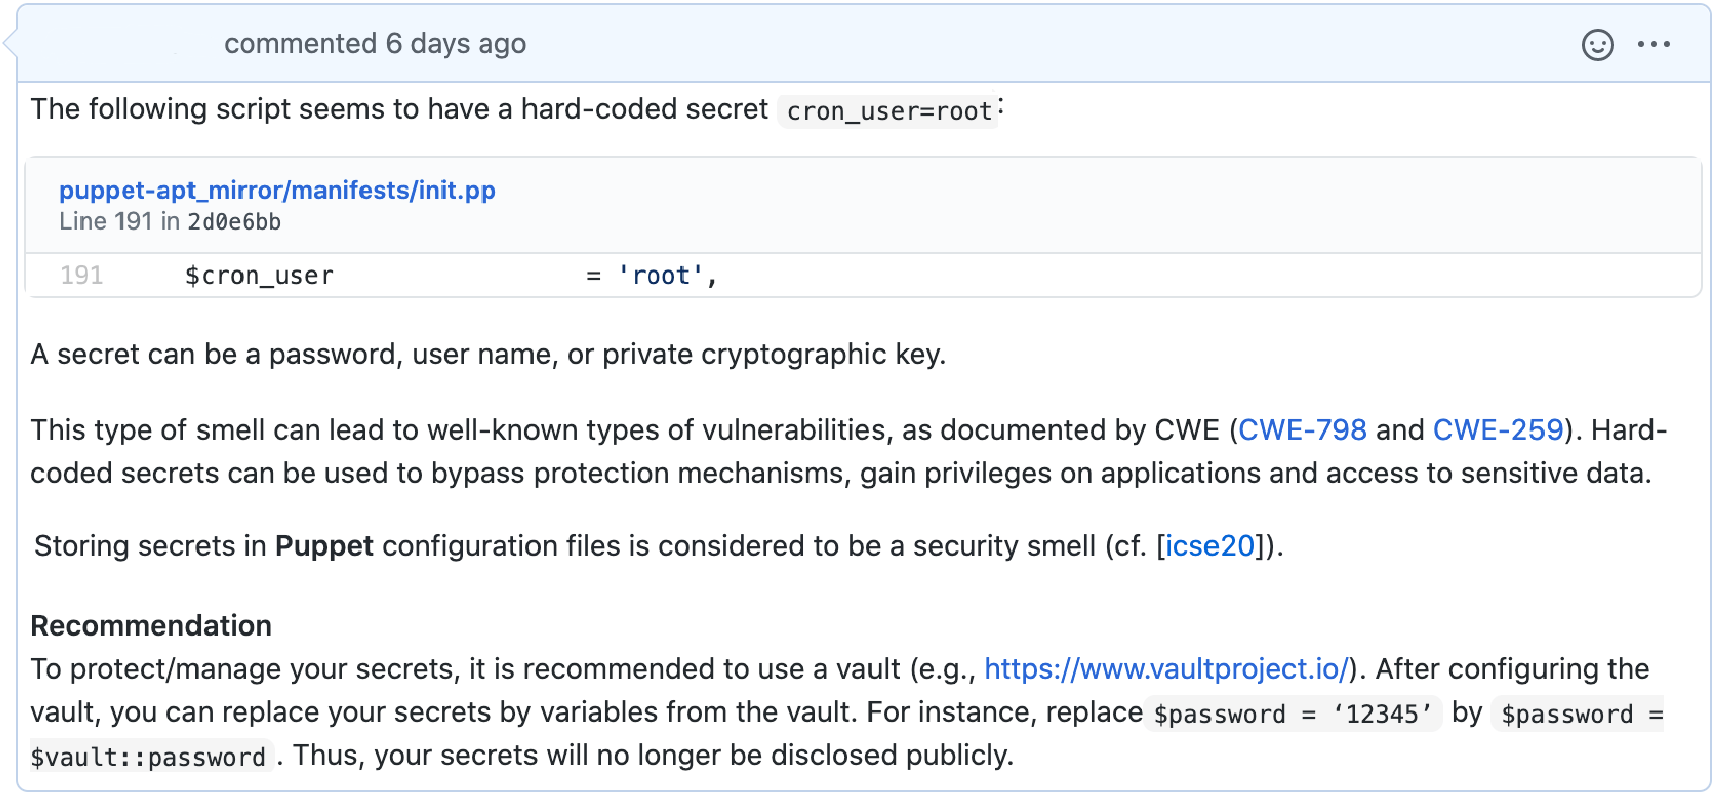
\includegraphics[width=\linewidth]{issue.png}
  \vspace{-4ex}  
  \caption{Example of issue opened (based on SLIC report).}\label{fig:issue}
  \vspace{-3ex}
\end{figure}
%

%
\subsubsection{Dataset}

The dataset used in this study was different from the one from 
Section~\ref{sec:pre_meth}. 
We mined \github\ projects with activity in $2020$ 
(at least one commit) and containing Puppet scripts. 
We conjectured that focusing on projects with recent activity would increase 
our chances of obtaining responses. We used two different queries to search for 
repositories: 1) \CodeIn{language:puppet is:public}; and, 2) \CodeIn{puppet in:readme is:public}. 
We discarded results pointing to forked repositories (to avoid
duplicates), repositories without any activity in $2020$ (no commits),
and repositories without any code in Puppet per project. Our tool
scanned \botTotalScripts{} Puppet scripts from \botWarningsRepos{}
GitHub repositories. In total, \botTotalWarnings{} security warnings
were detected in \botScriptsWarnings{} Puppet scripts (=$30.7\%$ of
the total). We issued alerts to projects with maintainers involved 
in the slack of the Puppet community. We received \botTotalIssuesAnswers{} answers to 
the \botTotalIssues{} issues we submitted, but only \botFinalIssues{}
issues were clearly validated by practitioners---which were 
the ones we considered for our conclusions.

\subsubsection{Methodology} This section presents the methodology 
followed to submit the issues. \textbf{Sample.} A total of
\botWarningsRepos{} \github\ repositories were scanned to this
study. We ensured that the repositories had recent activity (at least
one commit in $2020$) to improve the probability of obtaining
responses. The total amount of scripts scanned was
\botTotalScripts{}
---$7$ times the sample used in our preliminary
study (Section~\ref{subsec:dataset}) and $28$ times the sample used in
Rahman et. al~\cite{8812041} to evaluate the SLIC's precision and
recall. 
\textbf{Issues.} We reached out to the software owners 
through the Puppet community slack and submitted issues to projects 
with maintainers involved in the slack community. All the issues followed
a specific template depending on the type of warning
(cf. Figure~\ref{fig:issue}). The issued message not only located and
explained the vulnerability but also recommended an example of a
patch (i.e., actionable messages to save maintainers time). \textbf{Reply Evaluation.} We monitored the discussion threads
associated with the issues. For each response obtained, we classified
the warnings reported as true positives (TP) or false positives (FP)
according to the opinion of the maintainers in their responses.
Issues closed by the maintainers without any reply or activity were discarded.
Issues closed with unclear responses (e.g., 
``N/A'', ``:thumbs\_down'') were also discarded since they did not provide
clarity on the validation of the issue. We only considered the issues where there was some sort 
of discussion of the issue (e.g., ``These todo's shouldn't be there, I agree ... but it's not about defects/weaknesses here. It's 
just a marker to include more operating systems in the future.'') or a clear validation of the issue (e.g., ``All false positives'', ``This is not a secret.'').
From the answers
obtained, two of the co-authors manually inferred the classification
of each warning. We use Cohen's Kappa~\cite{cohen1960coefficient} to
measure the inter-rater reliability of human
decisions. \textbf{Metrics.} We measured Precision as
described in Section~\ref{sec:pre_meth}. 


\begin{table}[t!]
  \small
  \centering
   \setlength{\tabcolsep}{9pt}
  \caption{\label{tab:maintainers}Performance of \slic. (Validation with Owners\Space{ of OSS projects})}
  \vspace{-2ex}
  \begin{tabular}{lrrr} 
    \toprule
    Rule & \#TP & \#FP  & Precision\\
    \midrule
    Hard-coded secrets & $77$ & $119$ & $0.39$ \\
    Use of HTTP without TLS & $1$ & $72$ & $0.01$\\
    Suspicious comments & $3$ & $15$ & $0.17$\\
    Use of Weak Crypto. Algos. & $0$ & $3$ & $0.00$\\
    Invalid IP Address Binding & $0$ & $1$ & $0.00$\\
    Empty Password & $1$ & $5$ & $0.17$ \\
    Admin by default & $1$ & $0$ & $1.00$\\
    \midrule
    Total & 83 & 215 & 0.28\\
    \bottomrule 
  \end{tabular}
  \vspace{-2ex}  
\end{table}

\subsubsection{Results} This section reports results. \textbf{Issues.} We
reported a total of \botTotalWarnings{} warnings in \botTotalIssues{} issues
($9$ warnings per issue, on average). Project owners responded 
to \botTotalIssuesAnswers{} issues of the \botTotalIssues{}
issues we submitted, but only \botFinalIssues{} issues were clearly discussed 
or validated---the equivalent to \botTotalAnswered{} warnings (Table~\ref{tab:maintainers}). One issue for an
``Empty Password'' warning was fixed by one of the maintainers
(82c3cb7\footnote{Fix for ``Empty password'' issue: \url{https://github.com/jtopjian/puppet-sshkeys/commit/82c3cb7e78c16cf6517207779f79ab5b2a71b603} (Accessed \today)});
one tagged the issue with ``waiting for contribution''; another commented asking to perform a pull request. \textbf{Reply
  Evaluation.} We used the following method to determine the warning
classification (\ie{}, false or true positive) from the answers of
project owners. We discarded warnings related to issues closed without
any response or activity and issues that remained open or without any
response by the time of our analysis. After that stage, two of this paper's co-authors reviewed each of the answered
issues. Each warning received two votes. Then, we ran a Cohen's Kappa
analysis to measure the inter-rater reliability of our choices to
assess the confidence in our classification method. The kappa
coefficient ($k$) shows the level of agreement between the two
co-authors. The analysis yielded $k=1.0$, i.e., a total agreement 
between both co-authors. \textbf{Precision.} Table~\ref{tab:maintainers} shows the
number of true positives~(TP) and the number of false positives~(FP) per
type of warning. In total, \slic\ reported $83$ true positives and
$215$ false positives for the $33$ issues considered, which resulted in
an average precision of $0.28$ for \slic{}. Note that the samples used for 
``Use of Weak Crypto. Algorithms'', ``Invalid IP Address Binding'', ``Empty Password'' and 
``Admin by default'' are relatively small, so results might not reflect the entire reality. 


\textit{\textbf{Summary:}} Results indicate that the precision of
\slic{} is even lower when evaluated by maintainers---developers with 
more knowledge and context of the applications---of the software (drops to $28\%$).
These results confirm our initial observations and indicate that 
better security IaC linters for Puppet are needed.

\section{\toolname: Puppet Security Linter}\label{sec:tool}

The observations described in the previous section motivated the 
pursuit of a more precise security linter for Puppet scripts. 
The previous experiments ignited discussions with members 
of the development and security teams of PuppetLabs, as well 
as a project manager from Vox Pupuli. We leveraged the feedback 
obtained from the previous studies and the professional feedback to
design a new security linter for the Puppet
community, which we dubbed as \toolname{}. More precisely, we created 
a new linter as a result of \textit{phase 1} (Figure~\ref{fig:timeline}) 
and incrementally evolved the linter according to the recommendations of professionals 
(Figure~\ref{fig:timeline}, \textit{phase 2}), improving
\noRulesSlic\ rules of the \slic{} ruleset and adding
\newRules\ new rules. 
The following sections report the new architecture (Section~\ref{sec:architecture}), 
design choices (Section~\ref{sec:design}) and security checkers (Section~\ref{sec:rules}) that resulted
from the feedback collection (Figure~\ref{fig:timeline}): 
\begin{itemize}
  \item \textit{Phase 1}: feedback from the \textbf{owners of OSS projects},  
  \textbf{PuppetLabs} and \textbf{Voxpupuli Engineers} (as described in 
  Section~\ref{sec:preliminary_study}) that led to the creation of \toolname{} (v0.1.0);
  \item \textit{Phase 2}: two cycles of feedback from the \textbf{Puppet} and \textbf{Prolific} 
  communities (as described in Section~\ref{sec:evaluation}) that led to two new releases of 
  \toolname{} (v1.0.0 and v1.1.0);
\end{itemize}


\subsection{Linter Architecture}\label{sec:architecture}

One recommendation from the PuppetLabs team (\textit{phase 1}) was to implement 
the set of the rules as plugins to the \puplint{} architecture\footnote{Puppet-lint website: \url{http://puppet-lint.com/}},
through the \puplint\ check API\footnote{Puppet-lint check API: \url{http://puppet-lint.com/developer/api/}}. 
This API facilitates the integration of new checkers in \puplint\. 
In addition, it allows the user to suppress warnings and disable or enable
checkers---which are regarded as important features by the community. All 
security checks were developed as plugins to \puplint\ (Table~\ref{tab:rules}). 
These checks are applied to the Abstract Syntax Tree (AST) of a Puppet manifest which 
is generated by an internal tokenizer\footnote{Puppet-lint tokenizer: \url{http://puppet-lint.com/developer/tokens/}}.
\toolname\ was implemented in \texttt{Ruby} and its \texttt{CLI} is available 
online\footnote{Gem is available at \url{https://rubygems.org/gems/puppet-lint-infrasecure}}.
The codebase of the linter is available 
at \url{https://github.com/TQRG/puppet-lint-infrasecure} and open to future contributions.

\subsection{Design Choices}\label{sec:design}

This section describes the design choices of our analysis, guided by 
the distinct cycles of feedback as described in Section~\ref{sec:preliminary_study} 
and Section~\ref{sec:evaluation}; also, illustrated in Figure~\ref{fig:timeline}.

\textbf{Variable/Attribute Assignments (VASS).} From the preliminary 
analysis performed in Section~\ref{sec:preliminary_study}, we have noticed 
security-related code smells being detected in logical conditions. For instance, 
\CodeIn{if has\_key(\$userdata, ’env’)} shows a logical condition that 
was incorrectly flagged as a hard-coded secret issue. Aiming to 
reduce the number of incorrect predictions, we implemented a rule to search 
for variable and attribute assignments in Puppet manifests---\texttt{isVarAssign(\textit{token})}
and \texttt{isAtrAssign(\textit{token})} (cf. Table~\ref{tab:rules}).

\textbf{Reasoning about the token value (TOKVAL).} Some of the rules did not 
reason about \texttt{token.value}. For hard-coded secrets, 
the linter only checks if the token value is not empty. While manually validating the 
samples used in our studies, we found false positives of hard-coded secrets. For instance, 
\CodeIn{aws\_admin\_username = downcase(\$::operatingsystem)} which does not store 
any actual secret. \slic{} flagged this case as a hard-coded secret because the value assigned 
to the variable \CodeIn{aws\_admin\_username} is not empty. However, the rule needs to 
reason not only about the length of the right-hand side of the variable assignment but also about 
the type of token and value. \toolname\ locates variable and attribute assignments in the AST and considers 
that secrets are usually stored in \CodeIn{:STRING} and \CodeIn{:SSTRING} tokens. In addition, we defined a database
of known credentials (\texttt{isUserDefault(\textit{token.value})})---credentials that are not 
considered secrets by the community\footnote{\url{https://puppet.com/docs/pe/2019.8/what\_gets\_installed\_and\_where.html\#user\_and\_group\_accounts\_installed}}---and,
invalid secrets (\texttt{invalidSecret(\textit{token.value})}) which are 
consider as non-valid values for hard-coded secrets. The linter ignores all the credentials in this database. Feedback from distinct \textbf{owners of OSS Projects} is what
drove us to make this decision is presented below:

\begin{itemize}[topsep=.2ex,itemsep=.2ex,leftmargin=0em]
  \item[] \textbf{[User Default]}: 
  \textit{``The names of these UNIX accounts are not 
  considered to be secret. They are 
  published openly as part of the PE documentation:
  \url{https://puppet.com/docs/pe/2019.8/what\_gets\_installed\_and\_where.html\#user\_and\_group\_accounts\_installed}''}
  \item[] \textbf{[Invalid Secret]}: 
  \textit{``This are default users and default as found in every installed 
  fpm package. there is most of the time a wwwrun or a www-data user 
  depending on the system.''}
\end{itemize}

\textbf{Use of HTTP without TLS is fine sometimes (SAFE).} As \slic{}, \toolname{} also flags 
every single occurrence of \textit{http://}, i.e., it recommends to use TLS by default. For example, the tool
flags \CodeIn{apturl => "http://deb.debian.org/debian"}, even though it refers to a credible 
source. Our definition of credible source is a source that can be trusted. However, 
different companies can have different opinions regarding the credibility of the same source.
That is why this rule is customizable. We observed that this type of issues (CWE-319) are prevalent in Puppet files. 
Applications often use third-party libraries, which are usually configured in Puppet 
files, and the links to their sources are not necessarily unsafe.
Also, depending on the context of an application, the configuration of 
localhost servers as HTTP may not be a problem. If no sensitive data is communicated, 
then there is probably no problem using \CodeIn{http}. \toolname{} has a configuration file 
for safe domains, i.e., domains that are cleared to be use \CodeIn{http}. Thereby, infrastructure teams can 
customize their own configuration files. The feedback provided 
in Section~\ref{sec:evaluation} from two different \textbf{practitioners}, which
supported this decision, is presented bellow:

\begin{itemize}[topsep=.2ex,itemsep=.2ex,leftmargin=0em]
  \item[] \textbf{[Whitelist]}: 
  \textit{``I think it is fine if localhost is used. Otherwise TLS 
  should be mandatory. All the big 
  financial organizations will not use this check because 
  they cannot create internal certs or use 
  letsencrypt.''}
  \item[] \textbf{[Whitelist]}: 
  \textit{``By default, it's unsafe to not use HTTPS. 
  But for internal testing/development it is acceptable 
  to me to not use HTTPS all the time.''}
\end{itemize}


\textbf{Hard-Coded Secret Division in different checkers (SECR).} 
In Section~\ref{sec:preliminary_study},
we observed that the hard-coded secrets checker produces the most significant number
of alerts. For instance, \slic{} assumes a secret is a key, password or username. 
As mentioned previously in Section~\ref{sec:background},
the Common Weakness Enumeration list does not consider solo 
hard-coded usernames as a threat. Practitioners involved in our validation 
studies shared the same opinion. 
We analyzed the distribution of the different types of hard-coded secrets
and realized that $48\%$ of the secrets detected were usernames.
Therefore, in the final version of our tool, we decided
to separate the hard-coded secrets checker into three new checkers (one per type of secret). This 
way, developers can disable the username checker if they find it 
noisy. We did not delete the original checker; infrastructure
teams can use it if they want to collect all the different 
types of secrets simultaneously. Feedback provided 
in Section~\ref{sec:evaluation} from a \textbf{practitioner} 
supported this decision:

\begin{itemize}[topsep=.2ex,itemsep=.2ex,leftmargin=0em]
  \item[] \textbf{[Username]}: 
  \textit{``The main security issue is having the password hard-coded. 
  About having the user hard-coded, it is possible to allow that as an 
  initial setting that should be changed during the first configuration and, 
  in that case, it is not so much a security issue.''}
\end{itemize}


\begin{table}
  \centering
  \small
  \caption{\toolname{}'s list of string and AST patterns.}\label{tab:pattterns}
  \vspace{-2ex}
  \renewcommand{\arraystretch}{0.5}
  \begin{subtable}[h]{\linewidth}
    \begin{tabular}{p{3cm}p{5cm}} 
      \toprule
      \textbf{Rule} & \textbf{String Pattern}  \\
      \toprule
          isAdmin(\textit{t.value}) &  
            \url{root|admin} \\ \midrule
          isNonSecret(\textit{t.value}) & 
            \url{gpg|path|type|buff|zone|mode|tag|header|scheme|length|guid} \\\midrule
          isPassword(\textit{t.value}) & 
            \url{pass(word|\_|$)|pwd} \\\midrule
          isUser(\textit{t.value}) & 
            \url{user|usr} \\\midrule
          isKey(\textit{t.value}) & 
            \url{(pvt|priv)+.*(cert|key|rsa|secret|ssl)+} \\\midrule
          isPlaceholder(\textit{t.value}) & 
            \url{${.*}|($)?.*::.*(::)?} \\\midrule
          hasCyrillic(\textit{t.value}) & 
            \url{^(http(s)?://)?.*\\p{Cyrillic}+}\\ \midrule
          isInvalidIPBind(\textit{t.value}) & 
            \url{^((http(s)?://)?0.0.0.0(:\\d{1,5})?)$} \\ \midrule
          isSuspiciousWord(\textit{t.value}) & 
            \url{hack|fixme|ticket|bug|checkme|secur|debug|defect|weak} \\ \midrule
          isWeakCrypto(\textit{t.value}) & 
            \url{^(sha1|md5)} \\ \midrule
          isCheckSum(\textit{t.value}) & 
            \url{checksum|gpg} \\ \midrule
          isHTTP(\textit{t.value}) & 
            \url{^http://.+} \\ \midrule
          isUserDefault(\textit{t.value}) & 
            \url{pe-puppet|pe-webserver|pe-puppetdb|pe-postgres|pe-console-services|pe-orchestration-services|pe-ace-server|pe-bolt-server} \\ \midrule
          invalidSecret(\textit{t.value}) & 
            \url{undefined|unset|www-data|wwwrun|www|no|yes|[]|undef|true|false|changeit|changeme|none} \\\midrule
          isStrongPwd(\textit{t.value})~\footnote{The \texttt{strong\_password} ruby gem (\url{https://rubygems.org/gems/strong_password}) is used to determine if a password is strong or not.} & 
            StrongPassword::StrengthChecker(\textit{t.value}) \\\midrule
          isEmptyPassword(\textit{t.value}) & 
            t.value == ``''\\\midrule
          isVersion(\textit{t.value}) & 
            \url{.*_version}\\
        \bottomrule
      \end{tabular}
      \caption{String patterns are applied to token values.}
      \label{tab:string_patterns}
      \end{subtable}

      \par\bigskip

      \begin{subtable}[h]{\linewidth}
      \centering
      \begin{tabular}{p{2cm}p{6cm}} 
        \toprule
        \textbf{Rule} & \textbf{AST Pattern}  \\
        \midrule		
        isVariable(\textit{t}) & 
          t.type == \texttt{:VARIABLE} $\vee$ t.type == \texttt{:NAME} \\\midrule
        isString(\textit{t}) & 
          t.type == \texttt{:STRING} $\vee$ t.type == \texttt{:SSTRING} \\\midrule
        isVarAssign(\textit{t}) & 
          isVariable(\textit{t.prev\_code\_token}) $\wedge$ 
          t.type == \texttt{:EQUALS} $\wedge$ 
          isString(\textit{t.next\_code\_token}) \\\midrule
        isAtrAssign(\textit{t}) & 
          isVariable(\textit{t.prev\_code\_token}) $\wedge$ 
          t.type == \texttt{:FARROW} $\wedge$ 
          isString(\textit{t.next\_code\_token}) \\\midrule
        isResource(\textit{t}) &
          (t.prev\_code\_t.type == \texttt{:NAME} $\wedge$ 
          t.type == \texttt{:LBRACE} $\wedge$ 
          t.next\_code\_t.type == \texttt{:SSTRING}) $\vee$
          (t.prev\_code\_t.type == \texttt{:LBRACE} $\wedge$ 
          t.type == \texttt{:SSTRING})\\\midrule
        isFunctionCall(\textit{t}) &
          (t.type == \texttt{:NAME} $\wedge$ 
          t.next\_code\_token.type == \texttt{:LPAREN}) $\vee$
          t.type == \texttt{:FUNCTION\_NAME} \\\midrule
        isComment(\textit{t}) & 
          t.type is in (\texttt{:COMMENT}, \texttt{:MLCOMMENT}, \texttt{:SLASH\_COMMENT})\\
      \bottomrule
      \end{tabular}
      \caption{Patterns applied to the Abstract Syntax Tree (AST).}
      \label{tab:ast_patterns}
      \end{subtable}
      \vspace{-4ex}
\end{table}
%
%
\subsection{Rules}\label{sec:rules}
%
\toolname{} detects $12$ different security smells in Puppet manifests.
Table~\ref{tab:ast_patterns} presents the AST patterns 
that are searched in the AST for relevant nodes/sequences of nodes; 
and, table~\ref{tab:string_patterns} presents the string patterns used 
to validate the information in those nodes.
Table~\ref{tab:rules} shows the syntactic pattern matching rules per 
weakness which leverage the two sets of patterns mentioned
before.

\textbf{Hard-coded secrets (CWE-321, CWE-259, CWE-798):} The top of the Table~\ref{tab:rules}
contains $4$ different rules for hard-coded secrets: one per secret;
and a final one which detects all kinds of secrets at the same time (keys, 
password and usernames). In addition to the design choices,  
the rules consider that secret values cannot be placeholders 
(\CodeIn{!isPlaceholder()}, Table~\ref{tab:string_patterns}).

\textbf{Use of HTTP without TLS (CWE-319):} One of the main findings 
of our analysis is that HTTP without TLS is not always problematic. Therefore,
we created a configurable whitelist where infrastructure teams can add
safe domains. The checker will not raise alerts when in the 
presence of a safe domain (\CodeIn{inWhitelist()}, Table~\ref{tab:rules}). \toolname{} provides a default whitelist with 
known reliable sources such as \url{http://deb.debian.org/debian}. 
However, this default whitelist will be overwritten if the user 
configures a new one.


\begin{table}[t!]
  \small
  \centering
  \setlength{\tabcolsep}{4pt}
  \caption{Performance of \toolname\ v0.1.0.}
  \label{tab:prel_analysis_infrasecure}
  \vspace{-2ex}  
  \begin{tabular}{lrrrrrr} 
    \toprule
    \cellcolor{Gray} \textbf{\toolname{} v0.1.0} & \multicolumn{3}{c}{\textit{proportional}} & \multicolumn{3}{c}{\textit{uniform}}\\\midrule
    Rule & \#TP & \#FP & Pr. &  \#TP & \#FP & Pr. \\
    \midrule
    Hard-coded secrets & \tpHardcodedSecretsInfraSecureProportional{} & \fpHardcodedSecretsInfraSecureProportional{} & \precHardcodedSecretsInfraSecureProportional{} & 
    \tpHardcodedSecretsInfraSecureUniform{} & \fpHardcodedSecretsInfraSecureUniform{} & \precHardcodedSecretsInfraSecureUniform{} \\
    Use of HTTP without TLS & \tpHttpWithoutTLSInfraSecureProportional{} & \fpHttpWithoutTLSInfraSecureProportional{} & \precHttpWithoutTLSInfraSecureProportional{} & 
    \tpHttpWithoutTLSInfraSecureUniform{} & \fpHttpWithoutTLSInfraSecureUniform{} & \precHttpWithoutTLSInfraSecureUniform{} \\
    Suspicious comments & \tpSuspiciousCommentsInfraSecureProportional{} & \fpSuspiciousCommentsInfraSecureProportional{} & \precSuspiciousCommentsInfraSecureProportional{} & 
    \tpSuspiciousCommentsInfraSecureUniform{} & \fpSuspiciousCommentsInfraSecureUniform{} & \precSuspiciousCommentsInfraSecureUniform{} \\
    Use of Weak Crypto. Algorithms & \tpWeakCryptoInfraSecureProportional{} & \fpWeakCryptoInfraSecureProportional{} & \precWeakCryptoInfraSecureProportional{} & 
    \tpWeakCryptoInfraSecureUniform{} & \fpWeakCryptoInfraSecureUniform{} & \precWeakCryptoInfraSecureUniform{} \\
    Invalid IP Address Binding & \tpInvalidIPInfraSecureProportional{} & \fpInvalidIPInfraSecureProportional{} & \precInvalidIPInfraSecureProportional{} &
    \tpInvalidIPInfraSecureUniform{} & \fpInvalidIPInfraSecureUniform{} & \precInvalidIPInfraSecureUniform{} \\
    Empty Password & \tpEmptyPassInfraSecureProportional{} & \fpEmptyPassInfraSecureProportional{} & \precEmptyPassInfraSecureProportional{} & 
    \tpEmptyPassInfraSecureUniform{} & \fpEmptyPassInfraSecureUniform{} & \precEmptyPassInfraSecureUniform{} \\
    Admin by default & \tpAdminDefaultInfraSecureProportional{} & \fpAdminDefaultInfraSecureProportional{} & \precAdminDefaultInfraSecureProportional{} & 
    \tpAdminDefaultInfraSecureUniform{} & \fpAdminDefaultInfraSecureUniform{} & \precAdminDefaultInfraSecureUniform{}\\
    \midrule
    Total & \tpInfraSecureProportionalSample{} & \fpInfraSecureProportionalSample{} & \precTotalInfraSecureProportional{} & \tpInfraSecureUniformSample{} & \fpInfraSecureUniformSample{} & \precTotalInfraSecureUniform{} \\
    \bottomrule 
  \end{tabular}
  \vspace{-3ex}  
\end{table}


\textbf{Suspicious Comments (CWE-546):} This checker was controversial. It was 
recognized that it would be valuable to alert developers about comments in their code mentioning 
functionalities and weaknesses that might hint at attackers. However, keywords such 
as ``todo'', ``later'', and ``later2'' were considered noisy.  
We changed the list of keywords in response to the complaints and feedback 
obtained from the developers (\CodeIn{isSuspiciousWord()}, Table~\ref{tab:string_patterns}).

\textbf{Usage of Weak Crypto. Algorithms (CWE-326):} \toolname{}
searches for \emph{in calls to} functions (\CodeIn{isFunctionCall(), Table~\ref{tab:ast_patterns}}) implementing 
crypto algorithms such as ``md5'' and ``sha1''
in variable and attribute assignments (Table~\ref{tab:rules}). 

\textbf{Invalid IP Address Binding (CWE-284):} We found cases where 
the invalid IP \texttt{0.0.0.0} was in descriptions and commands. 
For instance, \slic{} flags \CodeIn{description => 'Open up postgresql for access to 
sensu from 0.0.0.0/0'}. IPs follow a 
dot-decimal notation, i.e., they should not include letters. 
\toolname\ uses a less naive regex 
than the string pattern 
(\CodeIn{isInvalidIPBind()}, Table~\ref{tab:string_patterns}).

\textbf{Empty Password (CWE-258):} Empty passwords 
are located the same way as hard-coded secrets, i.e., 
by focusing on variable and attribute assignments (Table~\ref{tab:rules}).
The rule \CodeIn{isEmptyPassword()} (Table~\ref{tab:string_patterns}) verifies 
if the password is empty. 

\textbf{Admin By Default (CWE-250):} These issues 
are also located by focusing on variable and attribute 
assignments (Table~\ref{tab:rules}). The rule \CodeIn{isAdmin()}, table~\ref{tab:string_patterns}, verifies 
if the user is ``admin'' or ``root''.


\textbf{Homograph Attacks (CWE-1007):} Typosquatting
attacks, also known as URL hijacking, is a social engineering attack 
that purposely uses misspelt domains for malicious purposes;
and are the cause of many supply chain attacks~\cite{duan2020measuring}.
This checker is important because malicious actors 
can use homoglyphs to modify reliable sources 
for malicious sources (\CodeIn{hasCyrillic()}, Table~\ref{tab:string_patterns}).


\textbf{Weak Password (CWE-521):} \toolname{} searches 
for passwords in the same way it searches for Empty Passwords and Hard-Coded 
Passwords. The only difference is the password value validation (\CodeIn{isStrongPwd()}, Table~\ref{tab:string_patterns})
which is performed by an external package (\texttt{strong\_password})
that implements an adaptation of a PHP algorithm developed by Thomas Hruska~\cite{blogpost}.

\textbf{Malicious Dependencies (CWE-829):} We produced a database of 
malicious dependencies for 
Puppet modules by crossing CVEs information and 
vulnerable products names with third-party libraries 
that can be configured in Puppet manifests.
We used the National Vulnerability Database (NVD)
to collect the CVEs and respective vulnerable 
products---from the list of Known Affected Software Configurations.
To get the list of products used by Puppet,
we used the Forge API\footnote{Forge API is available 
at https://forgeapi.puppet.com/}. 
Our database integrates malicious dependencies
for $33$ different packages (e.g., \texttt{rabbitmq}, 
\texttt{apt}, \texttt{cassandra}, \texttt{postgresql}, etc).
The checker searches for resource configurations (\CodeIn{isResource()}, Table~\ref{tab:ast_patterns})
and verifies if the 
a configured version of the software integrates 
our database of malicious dependencies for Puppet (\CodeIn{isMalicious()}, Table~\ref{tab:rules}).



\begin{table*}[h]
  \small
  \centering
  \caption{\toolname\ rules to detect security smells.}
  \vspace{-2ex}
  \setlength{\tabcolsep}{3pt} % General space between cols (6pt standard)
  \renewcommand{\arraystretch}{0.9} % General space between rows (1 standard)
      \begin{tabular}{p{1.3cm}p{3cm}p{12.5cm}} 
    \toprule
  \textbf{CWE} & \textbf{Weakness Name}	& \textbf{Rule} \\
  \midrule		
  CWE-321 & Hard-coded Key & 
    (isVarAssign(\textit{t}) $\vee$ isAtrAssign(\textit{t})) $\wedge$
    isKey(\textit{t.prev\_code\_token}) $\wedge$ 
    isNonSecret(\textit{t.prev\_code\_token}) $\wedge$ 
    !isPlaceholder(\textit{t.next\_code\_token}) \\\midrule
  CWE-259 & Hard-coded Password & 
    (isVarAssign(\textit{t}) $\vee$ isAtrAssign(\textit{t})) $\wedge$
    isPassword(\textit{t.prev\_code\_token}) $\wedge$ 
    isNonSecret(\textit{t.prev\_code\_token}) $\wedge$ 
    !isPlaceholder(\textit{t.next\_code\_token}) $\wedge$ 
    !isUserDefault(\textit{t.next\_code\_token}) $\wedge$
    !invalidSecret(\textit{t.next\_code\_token})\\\midrule
  CWE-798 & Hard-coded Usernames & 
    (isVarAssign(\textit{t}) $\vee$ isAtrAssign(\textit{t})) $\wedge$
    isUser(\textit{t.prev\_code\_token}) $\wedge$ 
    isNonSecret(\textit{t.prev\_code\_token}) $\wedge$ 
    !isPlaceholder(\textit{t.next\_code\_token}) $\wedge$ 
    !isUserDefault(\textit{t.next\_code\_token}) $\wedge$
    !invalidSecret(\textit{t.next\_code\_token}) \\\midrule
  CWE-798 & Hard-coded Secrets & 
    (isVarAssign(\textit{t}) $\vee$ isAtrAssign(\textit{t})) $\wedge$
    (isKey(\textit{t.prev\_code\_token}) $\vee$ 
    isPassword(\textit{t.prev\_code\_token}) $\vee$
    isUser(\textit{t.prev\_code\_token})) $\wedge$
    !isPlaceholder(\textit{t.next\_code\_token}) $\wedge$ 
    !isUserDefault(\textit{t.next\_code\_token}) $\wedge$
    !invalidSecret(\textit{t.next\_code\_token}) \\\midrule  
  CWE-319 & Use of HTTP without TLS & 
    (isVarAssign(\textit{t}) $\vee$ isAtrAssign(\textit{t})) $\wedge$
    isHTTP(\textit{t.next\_code\_token}) $\wedge$
    !inWhitelist(\textit{t.next\_code\_token})\\\midrule
  CWE-546 & Suspicious Comments & 
    isComment(\textit{t}) $\wedge$ 
    isSuspiciousWord(\textit{t})\\\midrule
  CWE-326 & Use of Weak Crypto. Algo. & 
    (isVarAssign(\textit{t.prev\_code\_token}) $\vee$ 
    isAtrAssign(\textit{t.prev\_code\_token}) $\vee$ 
    isFunctionCall(\textit{t.next\_code\_token})) $\wedge$
    !isCheckSum(\textit{t.prev\_code\_token}) $\wedge$
    isWeakCrypto(\textit{t.next\_code\_token}) \\\midrule
  CWE-284 & Invalid IP Address Binding & 
    (isVarAssign(\textit{t}) $\vee$ isAtrAssign(\textit{t})) $\wedge$
    isInvalidIPBind(\textit{t.next\_code\_token})\\\midrule
  CWE-258 & Empty Password & 
    (isVarAssign(\textit{t}) $\vee$ isAtrAssign(\textit{t})) $\wedge$ 
    isPassword(\textit{t.prev\_code\_token}) $\wedge$ 
    isEmptyPassword(t.prev\_code\_token)\\\midrule
  CWE-250 & Admin by default & 
    (isVarAssign(\textit{t}) $\vee$ isAtrAssign(\textit{t})) $\wedge$ 
    isNonSecret(\textit{t.prev\_code\_token}) $\wedge$ 
    isUser(\textit{t.prev\_code\_token}) $\wedge$ 
    !isPlaceholder(\textit{t.next\_code\_token}) $\wedge$ 
    isAdmin(\textit{t.next\_code\_token})\\\midrule
  CWE-1007 & Homograph Attacks & 
    (isVarAssign(\textit{t}) $\vee$ isAtrAssign(\textit{t})) $\wedge$ 
    hasCyrillic(\textit{t.next\_code\_token})\\\midrule
  CWE-521 & Weak Password & 
    (isVarAssign(\textit{t}) $\vee$ 
    isAtrAssign(\textit{t})) $\wedge$ 
    isPassword(\textit{t.prev\_code\_token}) $\wedge$ 
    isStrongPwd(\textit{t.next\_code\_token})\\\midrule
  CWE-829 & Malicious Dependencies & 
    isResource(\textit{t}) $\wedge$ 
    isVersion(\textit{t.prev\_code\_token}) $\wedge$
    isMalicious(\textit{t.next\_code\_token})\\
  \bottomrule
  \multicolumn{3}{l}{\setlength{\tabcolsep}{12pt}\CodeIn{inWhitelist(t.value)} verifies if the URL is in 
  the list of configurable safe domains/whitelist. If the URL 
  is in the whitelist, an alert should not be raised.}  \\  
  \multicolumn{3}{l}{\setlength{\tabcolsep}{12pt}\CodeIn{isMalicious(t.value)} verifies if the software package 
  version configured in the puppet script is in the database of malicious dependencies.}  \\  
  \bottomrule
  \end{tabular}
  \label{tab:rules}
  \vspace{-2ex}
\end{table*}

\subsection{Proof of Concept: \toolname{} v0.1.0}
%
As a proof of concept, two of the design choices described in Section~\ref{sec:design}
were implemented in the first version, \toolname{} v0.1.0, to 
ascertain whether precision could be enhanced. In particular, we focused on implementing 
variable and attribute assignments (VASS) and reasoning about the token value (TOKVAL),  
to reduce the number of incorrect detections. 

In our preliminary analysis with students (see Section~\ref{sec:preliminary_study}, 
Table~\ref{tab:prel_analysis_slic}), we observed that the precision of \slic{} was 
$64\%$. By implementing the two design choices mentioned before, we
increased precision by $12$ per cent points---when comparing \slic{}'s precision in
the \textit{proportional} set ($64\%$) with the precision of the first version of 
\toolname{} in the same dataset ($76\%$), Table~\ref{tab:prel_analysis_infrasecure}.
As these changes were successful w.r.t. precision, we decided to implement 
the other improvements and conduct a new study with practitioners to collect 
more feedback about the tool and the anti-patterns covered.


\section{Practitioners Evaluation}\label{sec:evaluation}

\toolname\ was validated with practitioners experienced in security 
or configuration management technologies. We built an experiment to validate 
the warnings of the new tool. The experiment was shared with the Puppet 
communities on Slack
(\texttt{puppetcommunity.slack.com}) and Reddit (\texttt{r/puppet}).
We found \noProfessionalsCommunity\ participants by this mean. Later, 
we leveraged Prolific\footnote{Prolific Platform: https://www.prolific.co/}~\cite{arxiv.2201.05348} 
to gather more participants
based on their experience and programming knowledge. 
In this experiment, a total of \totalWarningsPrac\ warnings were validated 
by \noProfessionals~practitioners. Furthermore, our improvements increased 
the precision of the tool from \botPrecision\ to \finalPrecision.
As illustrated in Figure~\ref{fig:timeline}, we run
two cycles of feedback collection and iteratively 
improve the tool with the feedback collected.
%
This section describes 1) the methodology 
conducted with practitioners to validate the \toolname\ 
warnings; and 2) the results obtained 
from running the practitioners' experiment.

\subsection{Study Design}

In this section, we detail how the validation study of \toolname\ 
was designed, and the population leveraged to conduct it.
\toolname\ was improved based on the problems collected through 
the preliminary study and the validations with the maintainers 
of the software---which led to \toolname{} v0.1.0. To validate the new tool, 
we surveyed practitioners with experience in security, configuration management 
tools and programming knowledge by following 
recent recommendations to run studies on Prolific~\cite{arxiv.2201.05348}. 
After the pre-screening, the practitioners 
were asked to validate and give feedback on \noWarningsPerPracticioner\ different 
warnings generated by \toolname.

\textbf{Practitioners Recruitment.} The participants were obtained using
two distinct routes: 1) By sharing the study with online Puppet communities such as 
    \texttt{puppetcommunity.slack.com} (slack) and \texttt{r/puppet} (reddit); 2) By using the Prolific platform to gather practitioners with 
    experience in security, configuration management tools and programming skills.
Both communities integrate a considerable amount of members: slack has 
over $9$k members, and Reddit has around $4.7$k members. However, only \noProfessionalsCommunity\ 
members participated in our study.
Therefore, we used Prolific to collect more practitioners with experience in security 
and configuration management tools outside of these two communities. 
Prolific participants were monetarily compensated for answering each survey, while the 
participants collected in the communities were not.

\textbf{Pre-Screening.} Prolific 
is a platform where you can find participants to perform online research. As recommended 
in research on recruiting practitioners for user studies on prolific~\cite{arxiv.2201.05348}, we performed 
a pre-screening of the population to collect adequate participants for this study, 
i.e., participants with security and configuration management experience; and 
programming knowledge. Prolific has filters dedicated to the industry where the 
participants work or belong. We sent the pre-screening survey to prolific 
users working in the following industries: ``Computer and Electronics Manufacturing'',
``Information Services and Data Processing'', ``Product Development'',
``Research laboratories'', ``Scientific or Technical Services'',
``Software''. The participants were asked to answer the following questions:
1) Do you have any kind of experience with configuration management tools?
\textbf{Choices:} Puppet, Ansible, Terraform, Chef, Other;
2) Experience in Security (Number of Years); 
3) Experience in Infrastructure as a Service (Number of Years);
and three programming language questions about different puppet
configurations. Due to space constraints, we do not present the
questions here, but they are available in our replication 
package: \url{study/practitioners/pre-screening/puppet-study-form.pdf}. 

We obtained a total of \noProfessionalsProlificRaw\ responses 
from $8$ different industries. Then, we ordered those participants by priority
where priority is the count of experience in 1) at least one configuration management tool ($CMEXP$), 
2) security ($SECEXP$), 3) infrastructure as a service ($INFRAEXP$); and 4) score in the programming 
questions ($SCORE$). 
Priority was calculated as follows $0.3 * ((CMEXP + SECEXP + INFRAEXP)/3) + 0.7 * (SCORE/3)$
and varies between $0$ to $3$. A priority of 
$3$ means the participant is adequate for the study, whereas a priority of $0$ means the participant 
is not adequate. For the validation study, we only invited  
participants with priority equal to or greater than $1.5$---which represented $53\%$ of the
initial responses (227 out of 431 participants).


\textbf{Validation Form.} We built a form online to share with the Puppet communities 
and practitioners. The initial page of the form explains the study's goal and asks 
the participant for her profession/career, number of years of experience in security, and number of years of experience in infrastructure/puppet. 
The goal of the study is to validate the output of our new tool: \toolname. 
Therefore, participants are required to validate $3$ different warnings (one at each time). For each warning, 
the form presents a description of the issue and the piece of code where the issue is located (cf. Figure~\ref{fig:warning}). 
Participants have to evaluate the issue and provide their validation:
``Yes, I agree'', if the warning reports a security issue; ``No, I disagree'',
if it reports a false security issue; or, ``I'm not sure'', when unsure.
The participant can also provide additional feedback on the problem.

\textbf{Warnings Dataset.}
For this experiment, we validated the output of $9$ different rules (Table~\ref{tab:rules}), where 
the warnings for weak passwords and malicious dependencies were mostly validated in 
the second round of feedback collection. We ran the \toolname\
over a total of $1050$ GitHub projects---collected from the dataset 
used in the preliminary study (Section~\ref{sec:preliminary_study}). We created
a uniform sample with $50$ warnings per rule (i.e., a total of $450$ warnings).

\begin{figure}[t!]
    \centering
    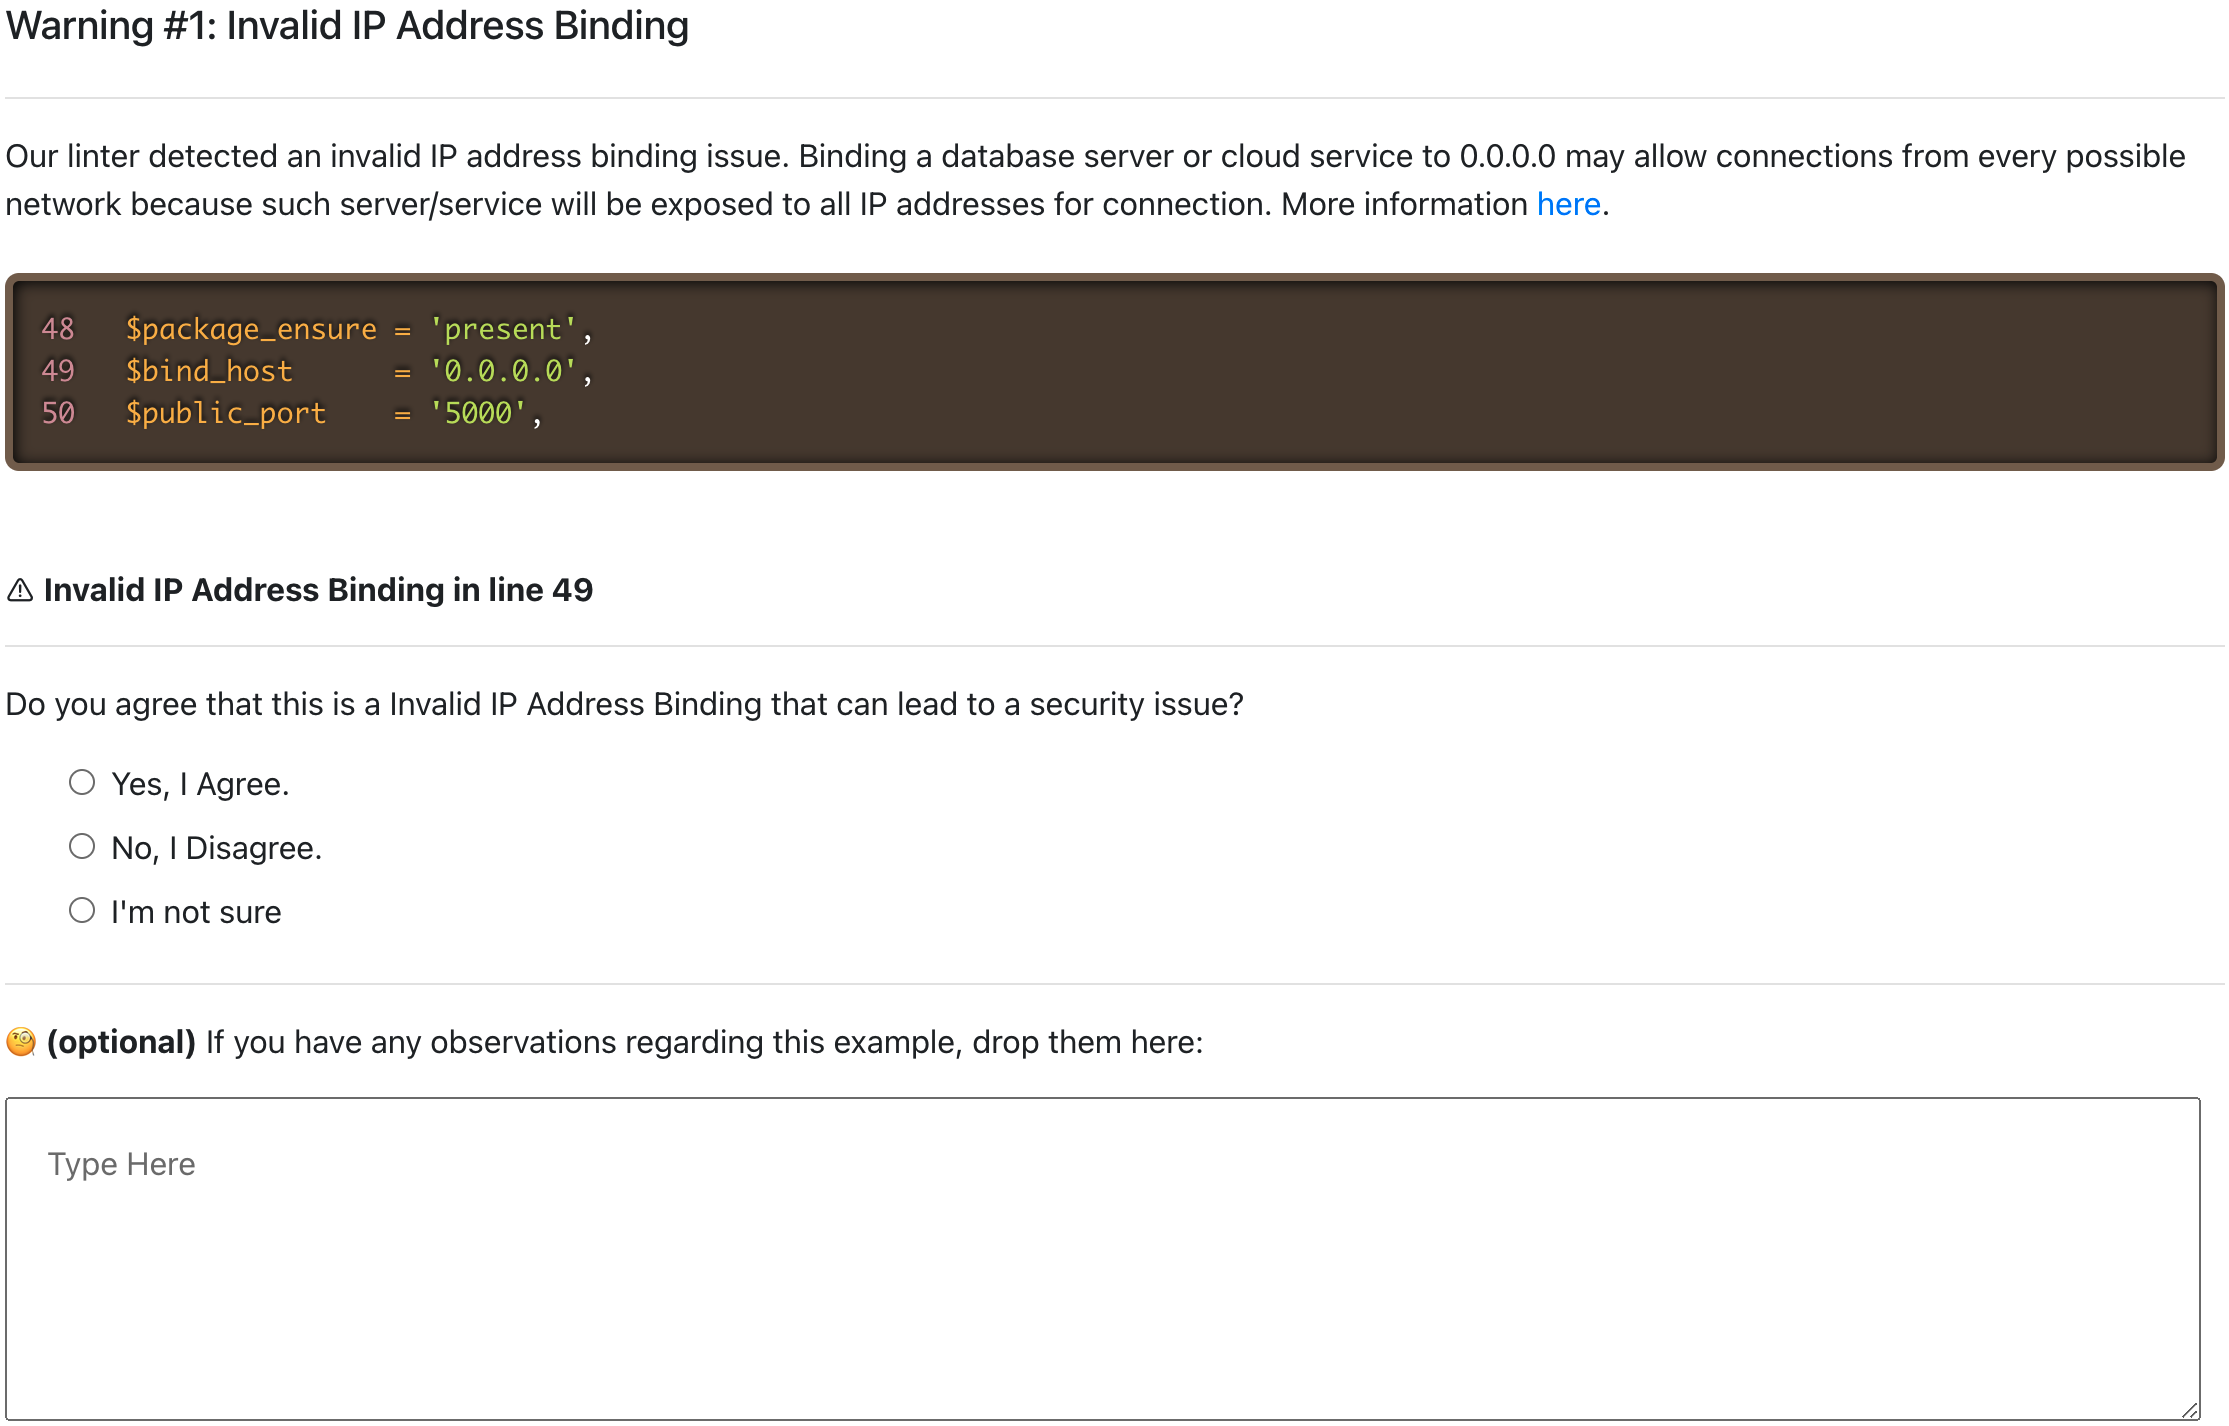
\includegraphics[width=1.05\linewidth]{warning.png}
    \vspace{-3ex}
    \caption{Example of the form presented to the 
    practicioner for warning validation.}\label{fig:warning}
    \vspace{-3ex}
\end{figure}

\textbf{Metrics.} We report the number of true positives (TPs), 
the number of false positives (TPs), the number of ``Unsure'' 
responses and Precision---calculated as described in 
Section~\ref{sec:pre_meth}.

\subsection{Results}
We obtained a total of \noProfessionals{} participants: $74$ in 
the first round of feedback; and $57$ in the second 
round. Due to the lack of responses from participants, we 
were only able to validate $342$ out of the 
$450$ initial number of warnings.
Table~\ref{tab:final_prac} shows the distribution of warnings and 
precision obtained for the final version of \toolname{} (v1.1.0). 
At the end of this study, \toolname{} reported a precision of 
\finalPrecision{}, where $54$ of the warnings  
were False Positives. 

Part of the feedback obtained in this experiment
was documented in Section~\ref{sec:design} and~\ref{sec:rules}.
Table~\ref{tab:infrasecure_prec} shows the evolution 
of the tool's precision with the different iterations of feedback.
In contrast to Table~\ref{tab:prel_analysis_infrasecure}, where 
we report the precision of v0.1.0 for the alerts validated by students;
here, in Table~\ref{tab:infrasecure_prec}, we report the precision of v0.1.0
based on the practitioners' feedback, i.e., leveraging the alerts validated 
by practitioners (instead of students). It is important to 
note that the implementation of v0.1.0 focused on understanding 
variable and attribute assignments and reasoning about the token value  
to reduce the number of incorrect detections. These two improvements affected 
all checkers. The remaining versions of the tool focused on addressing specific 
false positives, extending the ruleset and adding the safe domains feature. 
In the comparison provided in Table~\ref{tab:infrasecure_prec}, we 
observe an increase of precision---from $76\%$
to $83\%$---by conducting different cycles of 
feedback collection.
In addition, feedback was essential to extend 
the ruleset. This study with practitioners led us 
to create $3$ new rules to detect weak passwords;
typosquatting attacks; and malicious dependencies (being 
the last two the root causes of many supply chain attacks~\cite{9402108,duan2020measuring}).

\textit{\textbf{Summary:}} Results show that working side-by-side with the community
will help the authors of the tools develop better linters, 
as proposed before by a Google study~\cite{46576}.
Using this feedback approach, we improved the linter's precision 
and the final ruleset.


\begin{table}[t!]
  \centering
  \small
  \caption{Performance of \toolname{} (v1.1.0). (Validation with Practitioners)}
  \label{tab:final_prac}
  \vspace{-2ex}  
  \begin{tabular}{ p{3.75cm} p{0.5cm} p{0.5cm} p{1cm} p{1cm}} 
    \toprule
    Rule & \#TP & \#FP  & \#Unsure & Precision\\
    \midrule
    Hard-coded secrets & $28$ & $8$ & $3$ & $0.78$ \\
    Use of HTTP without TLS & $32$ & $3$ & $2$ & $0.91$\\
    Suspicious Comments & $16$ & $15$ & $7$ & $0.52$\\
    Use of Weak Crypto. Algo. & $33$ & $3$ & $6$ & $0.92$\\
    Invalid IP Address Binding & $26$ & $8$ & $6$ & $0.77$\\
    Empty Password & $33$ & $3$ & $1$ & $0.92$ \\
    Admin by default & $30$ & $6$ & $6$ & $0.83$\\
    Malicious Dependencies & $25$ & $6$ & $3$ & $0.81$\\
    Weak Password & $32$ & $2$ & $0$ & $0.94$\\
    \midrule
    Total & $255$ & $54$ & $34$ & $0.83$\\
    \bottomrule 
  \end{tabular}
\end{table}

\begin{table}[t!]
  \small
  \centering
  \caption{Precision obtained in different cycles of feedback collection for \toolname{}.}
  \label{tab:infrasecure_prec}
  \vspace{-2ex}  
  \begin{tabular}{p{5cm}p{1.25cm}p{1.25cm}} 
    \toprule
    \textbf{Participants} & \textbf{version} & \textbf{Precision} \\
    \midrule
    Research Team, Owners of OSS Projects, PuppetLabs, Voxpupuli & v0.1.0 &  76\% \\
    Practitioners (cycle 1) & v1.0.0 &  79\%\\
    Practitioners (cycle 2) & v1.1.0 & \finalPrecision \\
    \bottomrule 
  \end{tabular}
  \vspace{-3ex}
\end{table}


\subsection{Discussion \& Limitations}\label{sec:discussion}


This paper reports our approach to improve the ruleset of an IaC security iteratively 
linter in different cycles of feedback collection.
However, the tool can still be improved with more sophisticated 
techniques such as data-flow analysis, which would fulfil the following 
feedback: \textit{In puppet, pre-defining a password as empty does not 
mean it is empty (e.g., \CodeIn{\$ssl\_password    = ''}). Many times 
these variables are changed later. Thus, for each empty password,
\toolname{} verifies if the same variable was changed within the same file.
If it was, then the linter will not raise an issue.}.

In addition, some engineers suggested that usernames 
should be only reported as hard-coded secrets when 
paired with a password/key. For this, we must match the different 
pairs of credentials in a puppet manifest.
To sum up, there are still opportunities 
to improve the precision and recall of \toolname.
We reached out to owners of highly 
active GitHub projects that use Puppet reporting warnings 
detected by \toolname{}. Two owners mentioned that 
since the apps are not in production, they 
did not consider the issues relevant. Even 
after improving the linter to detect the anti-patterns 
correctly, some problems are still not problematic. This happens  
because the linter does not have context regarding 
the software's usage, which will always be a source 
of False Positives. In the future, we will continue to search 
for solutions to make the linter more context-aware
since this is a known problem of linters.

\section{Ethical Standards and Compliance}\label{sec:ethics}

This section discusses compliance with the ACM Policy for Research 
Involving Humans,\footnote{The ACM Policy for Research Involving Humans description is available at \url{https://www.acm.org/publications/policies/research-involving-human-participants-and-subjects} (Accessed \today)} which ensures that the ethical and legal standards 
are met when research has human participants.

\textbf{Informed Consent.} One of the principles is to ensure that 
participants are informed about the fact that they are participating 
in a study. In our study, consent was collected differently for each 
experiment: for the first one, the research team agreed to 
participate in the study; for the OSS maintainers experiment, we used 
the puppet community slack to communicate and discuss the investigation 
with the maintainers; finally, for the practitioners' experiment, we 
asked survey participants if they agreed to participate in our different 
surveys at the beginning of the pre-screening phase. 

\textbf{Data Privacy.} For all experiments, we ensured that the 
participants' private information was protected by not providing 
the participants' personal data (e.g., 
GitHub usernames of the OSS maintainers, prolific participants' 
names, ages, nationalities, etc.) in our replication package. 

\textbf{Spam.} As mentioned in Section~\ref{subsec:maintainers}, 
we carefully organized the issues 
to minimize the amount of messages sent to maintainers~\cite{10.1145/2961111.2962628,10.1145/3379597.3387462}. Security smells of the same kind were all reported in 
a single GitHub issue. In addition, we designed the issues to be 
actionable by providing personalized fix suggestions and 
adding references that document the detected problems.

\textbf{Full Disclosure in Security.} Fully disclosing vulnerabilities on GitHub issues 
allows hackers to exploit unfixed vulnerabilities, creating risks for software users. 
Ideally, vulnerability disclosure should be performed confidentially. Yet, GitHub does not 
provide a feature to report them privately. Therefore, carefully performing full disclosure 
is accepted by OSS maintainers~\cite{fulldisc.2005,askanethcode}. Some OSS projects adopt 
security mailing lists. In those cases, disclosure should be performed through those mailing 
lists. 

\section{Threats to Validity}\label{sec:t2v}

This section presents potential threats to the validity of this study.

\textbf{Internal Validity:} As with any implementation, the scripts that we 
developed to run the tools and collect the metrics 
reported in the paper are potentially not bug-free. However, the scripts and 
outputs are open-source for other researchers and
potential users to check the validity of the results. 

\textbf{Construct Validity:} A potential threat is the manual analysis
of the warnings raised by \slic{} in the Puppet scripts, which can potentially be 
mislabeled. We tried to mitigate this by running a kappa analysis between the two co-authors. 
For the experiments with the OSS maintainers, 
we inferred the validations of the alerts from their comments. Although both co-authors inferred the validations, and a kappa analysis was performed, we risk our inference being incorrect. It is also important to mention 
that even though we made an effort to collect feedback from experienced humans,
their judgement can also not be $100\%$ accurate, which can introduce error  
in the precision values reported.

\textbf{External Validity:} A potential threat to external validity 
is related to the fact that the set of Puppet scripts we have considered 
in this study may not accurately represent the whole set of 
vulnerabilities that can happen during development. We attempt to reduce
the selection bias by gathering a large collection of real, openly 
available (hence, reproducible) Puppet scripts. Another potential threat 
is that we could have missed the latest updates to \slic{}. To
mitigate this risk, we contacted the authors of \slic{} to confirm that 
the version available is true to the most recent one. 
%
\section{Related Work}\label{sec:rw}
%
As IaC has become popular and prevalent, researchers 
have dedicated efforts to improve its quality. Jiang \etal{} conducted
an empirical study on Puppet scripts to gain a deep understanding of the 
characteristics of such scripts and how they evolve over 
time~\cite{7180066}. Bent \etal{} investigated the quality and
maintainability aspects of Puppet scripts~\cite{van2018good}. 
Furthermore, Rahman \etal{} proposed prediction models (based on text
mining) to classify defective IaC scripts~\cite{rahman2018characterizing}. 
Palma \etal{} created a catalog of software metrics for IaC scripts ~\cite{dalla2020towards}. 
In addition, recent work has been developed to detect malicious
packages published on registry maintainers such as npm and ruby
gems~\cite{duan2020measuring}. Building and introducing linters 
earlier in the software development life-cycle shift security 
left and decreases the probability of shipping malicious packages.

There are several linters available for security but only the subject of
this paper, \slic{}, focuses in IaC scripts for Puppet~\cite{8812041}. 
The authors started by demonstrating the linter in the context of Puppet
scripts, and later, the authors reproduced the same study for Chef and 
Ansible and created new tools for those technologies~\cite{10.1145/3408897}. 
A major issues with linters is their lack of precision~\cite{park2016battles,muske2016survey,gauthier2018scalable,landman2017challenges,christakis2016developers,vassallo2020developers}: 
low precision entails low reliability for developers. Previous research 
has shown the impact of this issue on the developers' workflow and stressed 
it is essential to create precise tools; otherwise, the developers 
will not use them~\cite{6606613,7781843,10.1145/1646353.1646374,8622456,8530713,46576}.
As mentioned before, this study aims to gain a better 
understanding of the current capabilities of the only IaC security linter for 
Puppet and shed some light on how to move forward.

%
\section{Conclusions \& Future Work}\label{sec:conclusion}
%
In this study, we observed through a comprehensive study that 
security linters for IaC scripts still need to be improved to 
be adopted by the industry. This paper leverages community expertise 
to address the challenge of improving the precision of such linting 
tools. We focused on precision as it is critically important 
in this domain---false security warnings can be very disruptive. 
More precisely, we interviewed professional developers
of Puppet scripts to collect their feedback on the root causes of
imprecision of the state-of-the-art security linter for Puppet. From
that feedback, we developed a linter adjusting \noRulesSlic\ rules
of an existing linter ruleset and adding \newRules\ new rules. We
conducted a new study with \noProfessionals\ professional developers,
showing an increase in precision from \botPrecision\ to \finalPrecision.
Following the findings of a Google study~\cite{46576}, we show that 
authors of linters can improve their own tools if they focus 
on the users' feedback.
The takeaway messages of this paper are that (i) it is feasible to
tune security linters to produce acceptable precision; and, that 
(ii) involving practitioners in
discussions is an effective way to guide the improvement of those
linters. 

The observations that we made throughout this work pave the
way for the following future work: extend \toolname\ to detect other
security vulnerabilities, integrate the tool with methods for
automated patching, and port \toolname\ to other configuration
management tools.

\section{Using Generative AI to improve the recall of a security linter}
\label{sec:sectionb}


\cleardoublepage

% %%%%%%%%%%%%%%%%%%%%%%%%%%%%%%%%%%%%%%%%%%%%%%%%%%%%%%%%%%%%%%%%%%%%%%
% Dummy Chapter:
% %%%%%%%%%%%%%%%%%%%%%%%%%%%%%%%%%%%%%%%%%%%%%%%%%%%%%%%%%%%%%%%%%%%%%%

% %%%%%%%%%%%%%%%%%%%%%%%%%%%%%%%%%%%%%%%%%%%%%%%%%%%%%%%%%%%%%%%%%%%%%%
% The Introduction:
% %%%%%%%%%%%%%%%%%%%%%%%%%%%%%%%%%%%%%%%%%%%%%%%%%%%%%%%%%%%%%%%%%%%%%%
\fancychapter{SAST Testing and Validation}
\label{cap:chapter}

\textit{Present the chapter content.}

\section{Section A}
\label{sec:sectiona}

\subsection{Subsection A}
\label{subsec:subasectionA}

This would be a citation \cite{dummy}.

The \gls{cop} defines the performance of the machine.
% The first time you use this, the acronym will be written in full with the acronym in parentheses: supernova (SN). At later times it will just print the acronym: SN.

Heat Pump's performance is given by the \gls{cophp}, a \gls{cop} for heat pumps.

Now, an example on notation: \gls{Eu} and \gls{slip}.
Also \gls{Cd}.

\section{Section B}
\label{sec:sectionb}

\subsection{Subsection A}
\label{subsec:subasectionB}

The model described can also be represented as

\begin{equation}
\dot{\mathbf{x}}(t) = \mathbf{T}\mathbf{z}(y),\  \mathbf{y}(0) = \mathbf{y}_0,\  z\geq 0 \\
\label{eq:dummyeq1}
\end{equation}

\noindent where

\begin{equation}
\mathbf{A} = \left[ \begin{array}{cc} -(a_{12} + a_{10}) & a_{21} \\ a_{12} & -(a_{21} + a_{20}) \end{array} \right],\ \mathbf{x} = \left[ \begin{array}{c} x_1 \\ x_2 \end{array} \right] \\
\label{eq:dummyeq2}
\end{equation}

Also, using glossaries in the math environment, you can write
\begin{equation}
\gls{A} = \frac{\gls{mflow}\gls{_v}}{\rho u}
\label{eq:dummyeq3}
\end{equation}

Note that \gls{A} is not \gls{a}.


\subsection{Subsection B}
\label{subsec:subbsectionB}

Another example for the notation section: think about \gls{gamma}.
And \gls{gamma}\gls{_p} with a subscript.

\begin{table}[H]
	\centering
	\caption{Dummy Table.}
	\begin{tabular}{|c|c|c|c|} \hline
		\textbf{Vendor Name} 				& \textbf{Short Name}	& \textbf{Commercial Name}	& \textbf{Manufacturer}	\\ \hline \hline
		\multirow{3}{*}{Text in Multiple Row}		&	ABC				&  ABC\textreg				& ABC SA			         \\ \cline{2-4}
		 								&        DEF				&  DEF\textreg				& DEF SA				\\ \cline{2-4}
										&        GHF			&  GHF\textreg				& GHF SA				\\ \hline
		Text in Single Row					&        IJK				& IJK\textreg				& IJK SA				\\ \hline
		Frescos SA						&        LMN			& LMN\textreg				& LMN SA				\\ \hline
		Carros Lda.						&    \multicolumn{3}{|c|}{Text in Multiple Column}							\\ \hline
	\end{tabular}
	\label{tab:dummytable}
\end{table}

\cleardoublepage

% %%%%%%%%%%%%%%%%%%%%%%%%%%%%%%%%%%%%%%%%%%%%%%%%%%%%%%%%%%%%%%%%%%%%%%
% Dummy Chapter:
% %%%%%%%%%%%%%%%%%%%%%%%%%%%%%%%%%%%%%%%%%%%%%%%%%%%%%%%%%%%%%%%%%%%%%%

% %%%%%%%%%%%%%%%%%%%%%%%%%%%%%%%%%%%%%%%%%%%%%%%%%%%%%%%%%%%%%%%%%%%%%%
% The Introduction:
% %%%%%%%%%%%%%%%%%%%%%%%%%%%%%%%%%%%%%%%%%%%%%%%%%%%%%%%%%%%%%%%%%%%%%%
\fancychapter{Fixing Software Vulnerabilities Potentially Hinders Maintainability}
\label{cap:chapter}

\textit{Present the chapter content.}

\section{Introduction}
\label{sec:sectiona}
%
Software quality is important because it is ultimately related to 
the overall cost of developing and maintaining software 
applications, security and safety~\cite{slaughter1998evaluating}. Software quality 
characteristics include, but are not limited to functional 
correctness, reliability, usability, maintainability, evolvability 
and security. Security is an essential non-functional requirement 
during the development of software systems. In $2011$, the 
International Organization for Standardization (ISO) issued an 
update for software product quality ISO/IEC 25010 considering 
\emph{Security} as one of the main software product quality 
characteristics~\cite{iso:2011}. However, there is still 
a considerable amount of vulnerabilities being discovered and fixed, 
almost weekly, as disclosed by the Zero Day Initiative 
website\footnote{Zero Day Initiative website available at 
\url{https://www.zerodayinitiative.com/advisories/published/} 
(Accessed on \today{})}. 

Researchers found a correlation between the presence of 
vulnerabilities on software and code complexity~\cite{shin2010evaluating,10.1145/1774088.1774504}. 
Security experts claim that complexity hides bugs that may result in 
security vulnerabilities~\cite{mcgraw2004software,schneier2006beyond}. In 
practice, an attacker only needs to find one way into the system 
while a defender needs to find and mitigate all the security issues. 
Complex code is difficult to understand, maintain and 
test~\cite{1702388}. Thus, the task of a developer gets more challenging as the 
codebase grows in size and complexity. But the risk can be minimized 
by writing clean and maintainable code. 

ISO describes \textit{software maintainability} as ``the degree of 
effectiveness and efficiency with which a software product or system 
can be modified to improve it, correct it or adapt it to changes in 
environment, and in requirements'' on software quality ISO/IEC 
25010~\cite{iso:2011}. Thereby, maintainable security may be 
defined, briefly, as the degree of effectiveness and efficiency with 
which software can be changed to mitigate a security 
vulnerability---corrective maintenance.
% (hopefully, without introducing new ones). 
However, many developers still lack knowledge on the best 
practices to deliver and maintain secure and high-quality 
software~\cite{Pothamsetty:2005:SEL:1107622.1107635,8077802}. In a 
world where zero-day vulnerabilities are constantly emerging, 
mitigation needs to be fast and efficient. Therefore, it 
is important to write maintainable code to support the production of 
more secure software---maintainable code is less complex and, 
consequently, less prone to
vulnerabilities~\cite{shin2010evaluating,10.1145/1774088.1774504}---
and, prevent the introduction of new vulnerabilities. 

As ISO does not provide any specific guidelines/formulas to 
calculate maintainability, we resort to Software Improvement Group 
(SIG\footnote{SIG's website: 
\url{https://www.sig.eu/} (Accessed on \today{})})'s web-based source 
code analysis service Better Code Hub (BCH)\footnote{BCH's 
website: \url{https://bettercodehub.com/} (Accessed on \today{})}  
to compute the software compliance with a set of $10$ 
guidelines/metrics to produce quality software based on ISO/IEC 
$25010$~\cite{Visser:2016:OREILLY}. SIG 
has been helping business and technology leaders drive their organizational 
objectives by fundamentally improving the health and security of 
their software applications for more than 20 years. Their 
models are scientifically proven and certified~\cite{4335232,5609747,6113040,baggen2012}.

There are other well-known 
standards and models that have been proposed to increase software 
security: Common Criteria~\cite{common:2009} which received
negative criticism regarding the costs associated and poor technical 
evaluation; the OWASP Application Security Verification 
Standard (ASVS)~\cite{oswap:2009} which is focused only on web 
applications, and a model proposed by Xu et al. ($2013$)
~\cite{6616351} for rating software security (arguably, it was one 
of the first steps taken by SIG to introduce security on their 
maintainability model). Nevertheless, our study uses BCH to provide 
an assessment of maintainability in software for the following 
reasons: BCH integrates a total of $10$ different code metrics; and, 
code metrics were empirically validated in previous 
work~\cite{Bijlsma:2012:FIR:2317098.2317124,8530041,8919169,8785997}.

Static analysis tools (SATs) have been built to detect software 
vulnerabilities automatically (e.g., FindBugs, Infer, and more). Developers
use those tools to locate the issues in the code. However,
while performing the patches to those issues, SATs cannot provide 
information on the quality of the patch. 
Improving software security is not a trivial task and requires 
implementing patches that might affect software maintainability. 
We hypothesize that some of these patches may 
have a negative impact on the software maintainability and, 
possibly, even be the cause of the introduction of new 
vulnerabilities---harming software reliability and introducing 
technical debt. Research found that $34\%$ of the security patches 
performed introduce new problems and $52\%$ are incomplete and do not 
fully secure systems~\cite{10.1145/3133956.3134072}. Therefore, in this paper, 
we present an empirical study on the impact of patches of 
vulnerabilities on software maintenance across open-source software.
We argue that tools that assess these type of code metrics may
complement SATs with valuable information to help the developer
understand the risk of its patch.

From a methodological perspective, we leveraged a dataset of $1300$ 
security patches collected from open-source software. We calculate 
software maintainability before and after the patch to measure its 
impact. This empirical study presents evidence that changes applied 
in the codebases to patch vulnerabilities affect code 
maintainability. Results also suggest that developers 
should pay different levels of attention to different severity 
levels and classes of weaknesses when patching vulnerabilities. We 
also show that patches in programming languages such as, 
\emph{C/C++}, \emph{Ruby} and \emph{PHP}, may have a more negative 
impact on software maintainability. Little information is known 
about the impact of security patches on software 
maintainability. Developers need to be aware of the impact of their 
changes on software maintainability while patching security 
vulnerabilities. The harm of maintainability can increase the time 
of response of future mitigations or even of other maintainability 
tasks. Thus, it is of utmost importance to find means to assist 
mitigation and reduce its risks. With this study, we intend to 
highlight the need for tools to assess the impact of patches on 
software maintainability~\cite{4724577}; the importance of 
integrating maintainable security in computer science curricula; 
and, the demand for better programming languages, designed by 
leveraging security principles~\cite{kurilova2014wyvern,10.1145/2489828.2489830}. 
 
This research performs the following main contributions:
%
\begin{itemize}
  \item Evidence that supports the trade-off between security and 
  maintainability: developers may be hindering software 
  maintainability while patching vulnerabilities.
	\item An empirical study on the impact of security patches on 
	software maintainability (per guideline, severity, weakness and 
	programming language).
	\item A replication package with the scripts and data created to 
	perform the empirical evaluation for reproducibility. Available 
	online: \url{https://github.com/TQRG/maintainable-security}.
\end{itemize}
%
This paper is structured as follows: Section~\ref{sec:motivation} 
introduces an example of a security patch of a known vulnerability 
found in the protocol implementation of 
OpenSSL\footnote{\label{openssl}OpenSSL is a toolkit that
contains open-source implementations of the SSL and TLS cryptographic
protocols. Repository available at 
\url{https://github.com/openssl/openssl} (Accessed on \today{})}; 
Section~\ref{sec:methodology} describes the methodology used to 
answer the research questions; Section~\ref{sec:results} presents 
the results and discusses their implications; 
Section~\ref{sec:implications} elaborates on the implications
developers should consider in the future; Section~\ref{sec:threats} 
enumerates the threats to the validity of this study; 
Section~\ref{sec:rw} describes the different work and existing
literature in the field of study; and, finally, 
Section~\ref{sec:conclusions} concludes the main findings and 
elaborates on future work.

\section{Motivation and Research Questions}
\label{sec:motivation}

As an example, consider the patch of the TLS state machine protocol 
implementation in OpenSSL\footnoteref{openssl} to address a memory 
leak flaw found in the way how OpenSSL handled TLS status request 
extension data during session renegotiation, and where a malicious 
client could cause a Denial-of-Service (DoS) attack via large Online 
Certificate Status Protocol (OCSP) Status Request extensions when 
OCSP stapling support was enabled. OCSP stapling, formally known 
as the TLS Certificate Status Request extension, is a standard for 
checking the revocation status of certificates. 

This vulnerability is listed at the Common Vulnerabilities and 
Exposures dictionary as CVE-$2016$-$6304$~\footnote{CVE-$2016$-$6304$
details available at 
\url{http://cve.mitre.org/cgi-bin/cvename.cgi?name=CVE-2016-6304}
(Accessed on \today{})}. It is amongst the vulnerabilities studied 
in our research. The snippet, in Listing~\ref{lst:vuln}, presents 
the changes performed on the
\emph{ssl/t1$\_$lib.c} file\footnote{CVE-$2016$-$6304$ fix available 
 at
\url{https://github.com/openssl/openssl/commit/e408c09bbf7c3057bda4b8d20bec1b3a7771c15b}
(Accessed on \today{})} by the OpenSSL developers to patch the 
vulnerability. Every SSL/TLS connection begins with a handshake 
which is responsible for the negotiation between the two parties. 
The OSCP Status Request extension allows the client to verify the 
server certificate and enables a TLS server to include its response 
in the handshake. The problem in CVE-$2016$-$6304$ is a flaw in the 
logic of OpenSSL that does not handle memory efficiently when large 
OCSP Status Request extensions are sent each time a client requests 
renegotiation. This was possible because the OCSP responses IDs 
were not released between handshakes. Instead, they would be 
allocated again and again. Thus, if a malicious client does it 
several times it may lead to an unbounded memory growth on the 
server and, eventually, lead to a DoS attack through memory 
exhaustion. 

The code changes performed to patch the CVE-$2016$-$6304$ vulnerability are 
presented in Listing~\ref{lst:vuln}. The \texttt{sk\_OCSP\_RESPID\_pop\_free} function 
(\ref{lst:func1}) removes any memory allocated to the OCSP response IDs 
(\texttt{OCSP\_RESPID}s) from a previous handshake to prevent unbounded 
memory growth---which was not being performed before.
After releasing the unbounded memory, the logic condition in 
\ref{lst:func3} was shifted to \ref{lst:func2} which is responsible 
for handling the application when no OCSP response IDS are 
allocated. After the patch, in the new version of the software, the 
condition is checked before the package processing 
instead of after. Thereby, the system avoids the increase of 
unbounded memory (and a potential DoS attack).

Patching this vulnerability seems a rudimentary task. Yet,
a considerable amount of changes were performed in the codebase 
which yielded a negative impact on software maintainability.
While patching, the developer introduced $6$ new lines in a method 
already with a large number of lines of code and introduced more 
complexity to the code with $2$ new branch points, which disrupt two of 
the guidelines proposed by the Software Improvement Group 
(SIG) for building maintainable software~\cite{Visser:2016:OREILLY}: 
\emph{Write Short Units of Code} and \emph{Write Simple Units of 
Code}. 

\medskip
\setcounter{lstannotation}{0}
\begin{lstlisting}[style={CStyle}, caption={Patch provided by OpenSSL developers to the
CVE-2016-6304 vulnerability on file ssl/t1\_lib.c},label={lst:vuln}]
static int ssl_scan_clienthello_tlsext(SSL *s, PACKET *pkt, int *al){ 
 // [snip]
+  sk_OCSP_RESPID_pop_free(s->tlsext_ocsp_ids, OCSP_RESPID_free); /*!\annotation{lst:func1}!*/
+  if (PACKET_remaining(&responder_id_list) > 0) { 
+     s->tlsext_ocsp_ids = sk_OCSP_RESPID_new_null();
+     if (s->tlsext_ocsp_ids == NULL) { /*!\annotation{lst:func2}!*/
+        *al = SSL_AD_INTERNAL_ERROR;
+        return 0;
+     }
+  } else {
+     s->tlsext_ocsp_ids = NULL;
+  }

   while (PACKET_remaining(&responder_id_list) > 0) {
     OCSP_RESPID *id;
     PACKET responder_id;
     const unsigned char *id_data;
     if (!PACKET_get_length_prefixed_2(&responder_id_list, &responder_id) || PACKET_remaining(&responder_id) == 0) {
          return 0;
     }

-  if (s->tlsext_ocsp_ids == NULL 
-      && (s->tlsext_ocsp_ids = 
-      sk_OCSP_RESPID_new_null()) == NULL) { /*!\annotation{lst:func3}!*/
-    *al = SSL_AD_INTERNAL_ERROR;
-    return 0;
-  }

 // [snip]
 }
\end{lstlisting}

Software maintainability is designated as the degree to which an 
application is understood, repaired, or enhanced. In this paper, our 
concern is to study whether while improving software security, 
developers are also hindering software maintainability. This is 
important because software 
maintainability is approximately $75\%$ of the cost related to a 
project. To answer the following three research questions, we use 
two datasets of security 
patches~\cite{Reis:2017:IJSSE,10.1109/MSR.2019.00064} to measure the 
impact of security patches on the maintainability of open-source 
software. 
%

\textit{\textbf{RQ1: What is the impact of security patches on the
maintainability of open-source software?}} Often, security flaws 
require patching code to make software more secure. However, 
\textbf{there is no evidence yet of how security patches impact the
maintainability of open-source software}. We hypothesize that 
developers tend to introduce technical debt in their software when 
patching software vulnerabilities because they tend not to pay enough 
attention to the quality of those patches. To address it, 
we follow the same methodology as previous research~\cite{8919169} and compute 
the maintainability of $1300$ patches using the \emph{Better Code Hub} tool. 
We present the maintainability impact by guideline/metric, overall score, 
severity, and programming language.

\textit{\textbf{RQ2: Which weaknesses are more likely to
affect open-source software maintainability?}} There are security 
flaws that are more difficult to patch than others. For instance, 
implementing secure authentication is not as easy as patching a
cross-site scripting vulnerability since the latter can be fixed
without adding new lines of code/complexity to the code. A typical 
fix for the cross-site scripting vulnerability is presented in 
Listing~\ref{lst:fix}. The developer added the function 
\texttt{htmlentities} to escape the data given by the variable
\texttt{\$\_['file']}. We hypothesize that security patches for 
different weaknesses can have different impacts on software maintainability. 
\textbf{Understanding which weaknesses are more likely to increase maintainability 
issues is one step toward bringing awareness to security engineers of what 
weaknesses need more attention.} The taxonomy of security patterns used to answer this 
question is the one provided by the Common Weakness Enumeration
(CWE). \emph{Weakness}, according to the Common Weakness Enumeration 
(CWE) glossary, is a type of code-flaw that could contribute to the 
introduction of vulnerabilities within that product. In this study, maintainability 
is measured separately for each weakness.
%
\setcounter{lstannotation}{0}
\begin{lstlisting}[style={PHPStyle}, caption={Fix provided by \texttt{nextcloud/server} 
  developers to a Cross-Site Scripting vulnerability},label={lst:fix}]
   <p class='hint'>
    <?php
-   if(isset($_['file'])) echo $_['file']
+   if(isset($_['file'])) echo htmlentities($_['file'])
    ?>
   </p>
\end{lstlisting}
%
\textit{\textbf{RQ3: What is the impact of security patches versus 
regular changes on the maintainability of open-source software?}}
%
Performing a regular change/refactoring, for instance, to improve the name of 
a variable or function is different than performing a security patch.
Therefore, we also computed the maintainability of random regular commits using 
the \emph{Better Code Hub} tool---baseline. We use them to 
understand \textbf{how maintainability evolves when security patches 
are performed versus when they are not}.
%
\section{Methodology}\label{sec:methodology}
%

In this section, we discuss the methodology used to measure
the impact of security patches on the maintainability of open-source
software. The methodology comprises the following steps, as 
illustrated in Figure~\ref{fig:met}.
%
\begin{enumerate}
	\item Combine the datasets from related work that classify
	the activities of developers addressing security-oriented 
  patches~\cite{reis2017secbench,10.1109/MSR.2019.00064}. The
  duplicated patches were tossed.
%
	\item
	Extract relevant data (e.g., owner and name of
	the repository, sha key of the vulnerable version, sha key of 	
	the fixed version) from the combined dataset 	
	containing $1300$ security patches collected from open-source 	
	software available on GitHub.
%
  \item Two baselines of regular changes were collected:
  \textit{random-baseline} (for each security commit, a random change 
  was collected from the same project) and \textit{size-baseline} (for 
  each security commit, a random change with the same size
  was collected from the same project). Our goal is to evaluate the impact 
	of regular changes on the maintainability of open-source 
	software.
%
  \item Use the Software Improvement Group (SIG)'s web-based source 
  code analysis service \emph{Better Code Hub} (BCH)
  to quantify maintainability for both security and regular commits. 
  BCH evaluates the codebase available in the default branch of a GitHub project. 
  We created a tool that pulls the codebase of each commit of our dataset 
  to a new branch; it sets the new branch as the default branch; and, runs 
  the BCH analysis on the codebase; after the analysis is finished, the tool saves 
  the BCH metrics results to a cache file.
\end{enumerate}
%
\begin{figure}[h]
	\centering 	
    \begin{adjustwidth}{-0.5cm}{-0.5cm}  
      \vspace{-2.5cm} 
	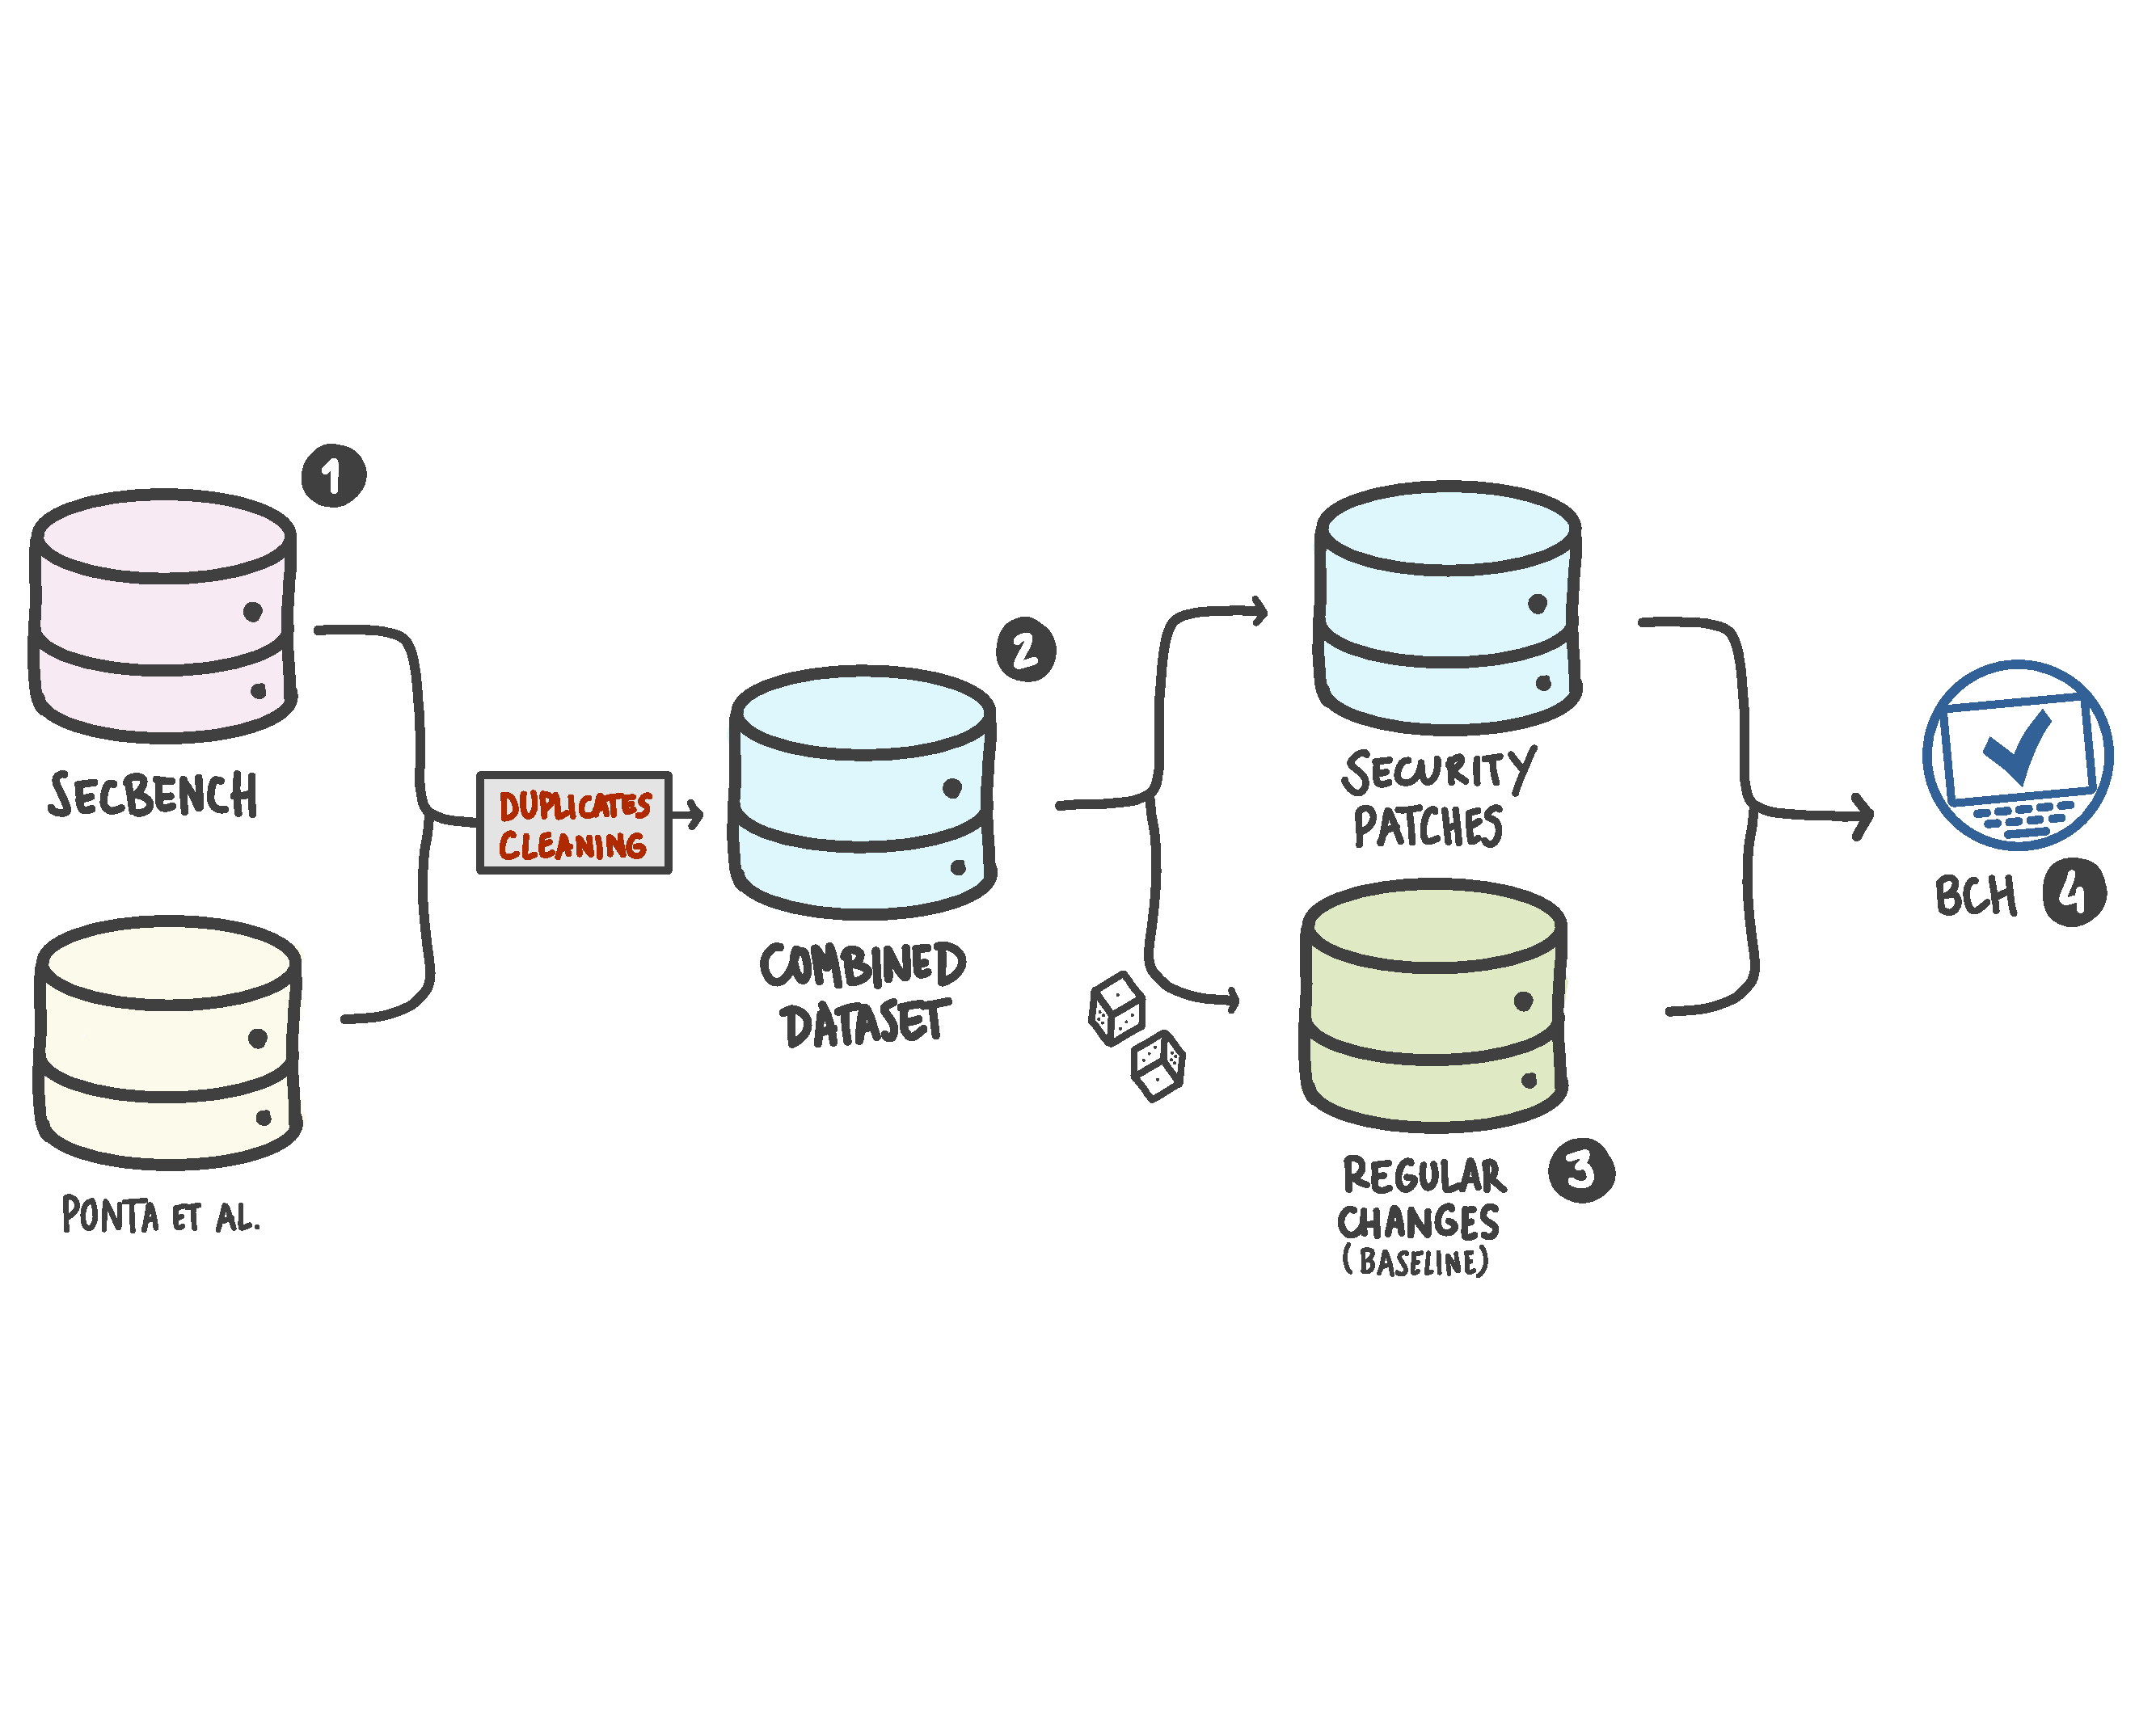
\includegraphics[width=1.1\textwidth]{Figures/methodology.pdf}
  \vspace{-3cm} 
  \caption{Study Methodology}
	\label{fig:met}
	 \end{adjustwidth}
\end{figure}
%
\subsection{Datasets}
%

We use a combined dataset of $1300$ security patches which is 
the outcome of mining and manually inspecting a total of $312$ 
GitHub projects. The combined dataset integrates two different
works: Secbench~\cite{reis2017secbench,Reis:2017:IJSSE} and Ponta et al.~\cite{10.1109/MSR.2019.00064}.

\textbf{Reis and Abreu 
($2017$)} mined open-source software aiming at the extraction of 
real---created by developers---patches of security vulnerabilities 
to test and assess the performance of static analysis 
tools~\cite{reis2017secbench,Reis:2017:IJSSE} since using hand-seeded test cases or 
mutations can lead to misleading assessments of the capabilities of 
the tools~\cite{just2014mutants}. The study yielded a dataset of 
$676$ patches for $16$ different security vulnerability types, dubbed as Secbench. 
The vulnerability types are based on the OWASP Top $10$ of 
$2013$~\cite{oswap:2013} and OWASP Top $10$ of 
$2017$~\cite{oswap:2017}. Each test case of the dataset is a 
triplet: the commit before the patching (\emph{sha-p}), the commit responsible
for the patching (\emph{sha}), and the snippets of code that differ from one 
version to another (typically, called \emph{diffs})---where one 
can easily review the code used to fix the vulnerability. 

\textbf{Ponta et al. ($2019$)} tracked the \url{pivotal.io} website for 
vulnerabilities from $2014$ to $2019$. For each new vulnerability, 
the authors manually searched for references to commits involved in 
the patch on the National Vulnerability Database (NVD) website. 
However, $70\%$ of the vulnerabilities did not have any references 
to commits. Thus, the authors used their expertise to locate the 
commits in the repositories. This technique yielded a dataset of 
$624$ patches~\cite{10.1109/MSR.2019.00064} and $1282$ commits---one 
patch can have multiple commits assigned. To fit the dataset in our methodology, we located the 
first and last commits used to patch the vulnerability. For these 
cases, we used the GitHub API to retrieve the dates of 
the commits automatically. Then, for each patch, the group of commits was ordered 
from the oldest commit to the newest one. We assumed the last commit 
(newest one) as the fix (\emph{sha}) and the parent of the 
first commit (oldest commit) as the vulnerable version 
(\emph{sha-p}). 
%

In this study, we focus on computing the maintainability of the 
commits before and after the security patching to evaluate if its 
impact was positive, negative, or none. The $1300$ patches in the 
dataset were analyzed using the BCH toolset to calculate their 
maintainability reports. Due to the limitations of BCH (in particular, 
lack of language support and project size) and the presence of
floss-refactorings, $331$ patches were tossed---explained in 
more detail in Section~\ref{sec:main_analysis}.
The final dataset used in this 
paper comprises $969$ security patches from $260$ projects. We used the 
Common Weakness Enumeration (CWE) taxonomy to classify each vulnerability. 
For instance,  the \texttt{Fix CVE-2014-1608: mc\_issue\_attachment\_get SQL injection} 
(\texttt{00b4c17}\footnote{CVE-$2014$-$1608$ details available at 
\url{https://github.com/mantisbt/mantisbt/commit/00b4c17088fa56594d85fe46b6c6057bb3421102} 
(Accessed on \today)}) is a \emph{CWE-89: Improper Neutralization of Special Elements used 
in an SQL Command ('SQL Injection')}\footnote{CWE-$89$ details available at \url{https://cwe.mitre.org/data/definitions/89.html} 
(Accessed on \today)} according to the CWE taxonomy.
We were able to classify a total of $866$ patches using the CWE taxonomy:
the CWE's for $536$ patches were automatically scraped from the National 
Vulnerability Dataset (NVD); while the other $370$ patches were manually classified by 
the authors following the \emph{Research Concepts} CWE's list\footnote{Research Concepts list available at \url{https://cwe.mitre.org/data/definitions/1000.html}}. A total 
of $103$ patches were not classified because we were not able to map
the issue to any CWE with confidence due to the lack of quality
information on the vulnerability/patch.

% In Table~\ref{tab:patterns}, the most prevailing categories are presented. To satisfy the Wilcoxon test size requirement, types of vulnerabilities
% with less than $20$ instances were merged in a bigger group named \textit{Miscellaneous}.

% \begin{table}[h]
% \scriptsize
% 	\caption{Guidelines to produce maintainable code}
% \begin{tabular}{L{1.1cm}L{2.1cm}L{4.3cm}}
%
% \toprule
% \textbf{Pattern} & \textbf{Name} & \textbf{Description}\\
% \midrule
%
% \textbf{CWE-89} &
%  Improper Neutralization of Special Elements used in an SQL Command/SQL Injection (23 cases) &
%  When developers do not keep untrusted data
%      separate from SQL queries. If an attacker sends a command that
%      exploits the syntax of the SQL interpreter, then SQL injection attack is possible.\\\midrule
%
% \textbf{CWE-611} &
%  Improper Restriction of XML External Entity Reference (24 cases) &
% 	XML documents are exchanged through the web containing entities with URIs
%  	that resolve to local/external files. Thus, when XML parsers are not well configured,
%  	attackers have allowed to directly those files.\\\midrule
%
%  \textbf{CWE-20} &
%  Improper Input Validation (76 cases) &
% 	When developers
%  	forget to validate the inputs of an application, attackers may have control
%  	of the control/data flow of the program.\\\midrule
%
%   \textbf{CWE-200} &
% Information Exposure (39 cases)&
% Application's logs are one way of intentional/unintentional disclosure information
%  	to attackers. Many times attackers get access to logs when sould not be authorized to.\\\midrule
%
%    \textbf{CWE-352} &
% Cross-Site Request Forgery/CSRF (22 cases)&
% Poor session tokens generation
%      and management usually allow attackers to send forged HTTP requests
%      including authentication information from the victim to the vulnerable web
%      application.\\\midrule
%
%        \textbf{CWE-264} &
% Permissions, Privileges, and Access Controls (59 cases)&
% Incorrectly
%  	    implemented functionalities related to authentication and session
%  	    management, allowing an attacker to gain access to session tokens,
%  	    passwords, keys, and other sensitive data.\\\midrule
%
%  	           \textbf{CWE-399} &
% Resource Management Errors (22 cases)&
% Resource management issues are found more frequently
%  		in programming languages that do not manage memory automatically (e.g., C/C++
%  	    and Objective-C), i.e., where developers are responsible for
%  	    handling it instead. It is one of the main causes of Denial-of-Service attacks.\\\midrule
%
%  	     	           \textbf{CWE-79} &
% Improper Neutralization of Input During Web Page Generation/Cross-site Scripting (63 cases)&
% Lack of proper validation or escaping
%  	    allows attackers to submit untrusted data to web browsers through malicious
%  	    scripts that can hijack the user sessions or redirect the user to malicious
%  	    sites.\\\midrule
%
%  	     	           \textbf{CWE-22} &
% Improper Limitation of a Pathname to a Restricted Directory/Path Traversal (37 cases) &
% When developers forget to neutralize special elements within the path names to files/directories, attackers
%  	may leverage this flaw to resolve to a location outside of the restricted directory and gain access to documents
%  	or entire repositories.\\\midrule
%
%  	 	     	           \textbf{MISC} &
% Miscellaneous (666 cases) &
% This pattern comprises
%  		several other security patches that do not have a CWE assigned and patterns that
%  		do not satisfy the Wilcoxon test size requirement of more than $20$ patches.\\
% \bottomrule
% \end{tabular}
% \label{tab:patterns}
% \end{table}

%
% \begin{itemize}
%     \item \textbf{CWE-89: Improper Neutralization of Special Elements used in an SQL Command/SQL Injection (23 cases).} When developers do not keep untrusted data
%     separate from SQL queries. If an attacker sends a command that
%     exploits the syntax of the SQL interpreter, then SQL injection attack is possible.
% %
%     \item \textbf{CWE-611: Improper Restriction of XML External Entity Reference (24 cases).}
% 	XML documents are exchanged through the web containing entities with URIs
% 	that resolve to local/external files. Thus, when XML parsers are not well configured,
% 	attackers have allowed to directly those files.
% %
%     \item \textbf{CWE-20: Improper Input Validation (76 cases).} When developers
% 	forget to validate the inputs of an application, attackers may have control
% 	of the control/data flow of the program.
% %
%     \item \textbf{CWE-200: Information Exposure (39 cases).} Application's logs are one way of intentional/unintentional disclosure information
% 	to attackers. Many times attackers get access to logs when sould not be authorized to.
% %
% 	\item \textbf{CWE-352: Cross-Site Request Forgery/CSRF (22 cases).} Poor session tokens generation
%     and management usually allow attackers to send forged HTTP requests
%     including authentication information from the victim to the vulnerable web
%     application.
% %
% 	\item \textbf{CWE-264: Permissions, Privileges, and Access Controls (59 cases).} Incorrectly
% 	    implemented functionalities related to authentication and session
% 	    management, allowing an attacker to gain access to session tokens,
% 	    passwords, keys, and other sensitive data.
% %
% 	\item \textbf{CWE-399: Resource Management Errors (22 cases).} Resource management issues are found more frequently
% 		in programming languages that do not manage memory automatically (e.g., C/C++
% 	    and Objective-C), i.e., where developers are responsible for
% 	    handling it instead. It is one of the main causes of DoS attacks.
% %
% 	\item \textbf{CWE-79: Improper Neutralization of Input During Web Page Generation/Cross-site Scripting (62 cases)} Lack of proper validation or escaping
% 	    allows attackers to submit untrusted data to web browsers through malicious
% 	    scripts that can hijack the user sessions or redirect the user to malicious
% 	    sites.
% %
% 	\item \textbf{CWE-22: Improper Limitation of a Pathname to a Restricted Directory/Path Traversal (37 cases).}  When developers forget to neutralize special elements within the pathnames to files/directories, attackers
% 	may leverage this flaw to resolve to a location outside of the restricted directory and gain access to documents
% 	or entire repositories.
% %
% 	\item \textbf{Miscellaneous (673 cases)} This pattern comprises
% 		several other security patches that do not have a CWE assigned and patterns that
% 		do not satisfy the Wilcoxon test size requirement of more than $20$ patches.
% \end{itemize}
%
\subsection{Security Patches vs. Regular Changes}
%
Previous studies attempted to measure the impact of regular changes 
on open-source software maintainability~\cite{HEGEDUS2018313}. 
However, there is no previous work focused on comparing the impact 
of security patches with regular changes on maintainability, only
with bug-fixes~\cite{10.1145/3133956.3134072}.
We analyze the maintainability of regular changes---changes not 
related to security patches---and, use them as a baseline.
The baseline dataset is generated from the security commits dataset, i.e.,
for each security commit in the dataset, we collect a random regular
change from the same project. We created two different baselines: 
\textit{random-baseline},
considering random changes and all their characteristics; and,
\textit{size-baseline}, considering also random changes
but with an approximate size as security patches---we argue 
that comparing changes with considerably different sizes may be unfair.

\subsubsection{Random-Baseline} 

As for the security patches, for each regular change, we  
need the commit performing the regular change (\emph{sha-reg}) and 
version of the software before the change (\emph{sha-reg-p}). A 
random commit from the same project is selected for each security patch, \emph{sha-reg}. The parent commit
of \emph{sha-reg} is the \emph{sha-reg-p}.

\subsubsection{Size-Baseline} 

For the size-baseline, we also need to obtain the regular change (\emph{sha-reg})
and the version of the software before the change (\emph{sha-reg-p}). 
First, our tool calculates the \emph{diff}
between the security patch and its parent.
Second, a random commit/regular change from 
the same project is selected, \emph{sha-reg}. The 
\emph{diff} between \emph{sha-reg} and its parent (\emph{sha-reg-p})
is calculated. Then, the regular change \emph{diff} is compared 
to the security patch \emph{diff}.
Due to the complexity of some patches, it was not possible 
to find patches with the exact same number of added and deleted lines. 
Thus, we looked for an approximation.

The pair of the regular change (\emph{sha-reg}) and its parent (\emph{sha-reg-p}) is accepted if the 
\emph{diff} size fits in the range size. This range widens every 
$10$ attempts to search for a change with an approximate size. We 
originate the regular changes from the security commits to ensure 
that differences in maintainability are not a consequence of 
characteristics of different projects.


\subsection{Bettter Code Hub}

SIG---the company behind BCH---has been helping business and technology 
leaders drive their organizational objectives by fundamentally improving 
the health and security of their software applications for more than $20$ years. 
The inner-workings of their SIG-MM model---the one behind BCH---are 
scientifically proven and certified~\cite{4335232,5609747,6113040,baggen2012}.

BCH checks GitHub codebases against $10$ maintainability 
guidelines~\cite{Visser:2016:OREILLY} that were empirically 
validated in previous work~\cite{Bijlsma:2012:FIR:2317098.2317124,8530041,8919169,8785997}.
SIG has devised these guidelines after many years of experience: analyzing more 
than $15$ million lines of code every week, SIG maintains the industry’s largest 
benchmark, containing more than $10$ billion lines of code across $200$+ technologies; SIG 
is the only lab in the world certified by TÜViT to issue ISO $25010$ certificates\footnote{Information available here: 
\url{https://www.softwareimprovementgroup.com/methodologies/iso-iec-25010-2011-standard/}}.
BCH's compliance criterion is derived from the requirements for 4-star 
level maintainability (cf. ISO $25010$)~\cite{5609747,6113040,baggen2012,Visser:2016:OREILLY}.
SIG performs the threshold calibration
yearly on a proprietary data set to satisfy the requirements of TUViT to
be a certified measurement model.

As BCH, other tools also perform code analysis for similar 
metrics. Two examples are Kiuwan and SonarCloud. However, Kiuwan does
not provide the full description of the metrics it measures; and, SonarCloud
although it provides a way of rating software maintainability, the variables 
description of their formula are not available. Both analyze less maintainability
guidelines than BCH and do not have their inner workings fully and publicly described.

\subsection{Maintainability Analysis}\label{sec:main_analysis}


In this research, we follow a very similar methodology to the one 
presented in previous work on the maintainability of energy-oriented 
fixes~\cite{8919169}. The inner workings of BCH were proposed
originally in 2007~\cite{4335232} and suffered refinements later~\cite{5609747,6113040,baggen2012}. 
As said before, the web-based source code 
analysis service \emph{Better Code Hub} (BCH) is used to collect the 
maintainability reports of the patches of each project. 
Table~\ref{tab:guidelines} presents the $10$ guidelines proposed
by BCH's authors for delivering software that is not difficult to
maintain~\cite{Visser:2016:OREILLY} and, maps each guideline to the 
metric calculated by BCH. These guidelines are calculated using the 
metrics presented in~\cite{criteria:2017} and are also briefly explained in Table~\ref{tab:guidelines}. 
During each guideline evaluation, the tool determines the compliance 
towards one guideline by establishing limits for the percentage of 
code allowed to be in each of the $4$ risk severity levels
(\emph{low risk}, \emph{medium risk}, \emph{high risk}, and 
\emph{very high risk}). If the project does not violate those 
thresholds, then the BCH considers that the code is compliant with 
a guideline. These thresholds are determined by BCH using their own
data/experience---using open-source and closed software systems. If 
a project is compliant with a guideline, it means that it is at 
least $65\%$ better than the software used by BCH to calculate the 
thresholds\footnote{Check the answer to \emph{How can I adjust the 
threshold for passing/not passing a guideline?} at
\url{https://bettercodehub.com/docs/faq} (Accessed on \today{})}.

\begin{table}[h]
\centering
\scriptsize
	\caption{Guidelines to produce maintainable code.}
\begin{tabular}{L{2cm}L{4.5cm}L{4cm}}

\toprule
\textbf{10 Guidelines} & \textbf{Description} & \textbf{Metric}\\
\midrule

\textbf{Write Short Units of Code} & Limit code units to $15$ LOCs because smaller
 units are easier to understand, reuse and test them & \textbf{Unit Size:} \% of 
 LOCs within each unit~\cite{criteria:2017} \\\midrule

\textbf{Write Simple Units of Code} & Limit branch points to $4$ per unit because
it makes units easier to test and modify & \textbf{McCabe Complexity:} \# of decision 
points~\cite{1702388,criteria:2017}\\\midrule

\textbf{Write Code Once} & Do not copy code because bugs tend to replicate at
multiple places (inefficient and error-prone) & \textbf{Duplication:} \% of redundant 
LOCs~\cite{criteria:2017}\\\midrule

\textbf{Keep Unit Interfaces Small} & Limit the number of parameters to at most
$4$ because it makes units easier to understand and reuse & \textbf{Unit Interfacing:} 
\# of parameters defined in a signature of a unit~\cite{criteria:2017} \\\midrule

\textbf{Separate Concerns in Modules} & Avoid large modules because changes in
loosely coupled databases are easier to oversee and execute & \textbf{Module Coupling:} \# of
incoming dependencies~\cite{criteria:2017} \\\midrule

\textbf{Couple Architecture Components Loosely} & Minimize the amount of code
within modules that are exposed to modules in other components & \textbf{Component Independence:} 
\% of code in modules classified as hidden~\cite{criteria:2017}\\\midrule

\textbf{Keep Architecture Components Balanced} & Balancing the number of
components ease locating code and allow for isolated maintenance & \textbf{Component Balance:} 
Gini coefficient to measure the inequality of distribution between components~\cite{criteria:2017} \\\midrule

\textbf{Keep your code base Small} & Reduce and avoid the system size because
small products are easier to manage and maintain & \textbf{Volume:} \# of LOCs converted 
to man-month/man-year~\cite{criteria:2017} \\\midrule

\textbf{Automate Tests} & Test your code base because it makes development
predictable and less risky & \textbf{Testability:} Ratings aggregation $-$ unit 
complexity, component independence and volume~\cite{Visser:2016:OREILLY}
 \\\midrule

\textbf{Write Clean Code} & Avoid producing software with code smells because
it is more likely to be maintainable in the future & \textbf{Code Smells:} 
\# of Occurrences~\cite{Visser:2016:OREILLY} (e.g., magic constants and long 
identifier names) \\
\bottomrule
\end{tabular}
\label{tab:guidelines}
\end{table}

Figure~\ref{fig:bchrep} shows an example of the report provided by BCH 
for a project after finishing its evaluation. The example
refers to the OpenSSL CVE-$2016$-$6304$ vulnerability patch---
as described by Section~\ref{sec:motivation}. This version of 
OpenSSL only complies with $1$ out of $10$ guidelines: \emph{Write 
Clean Code}.

\begin{figure}[h]
  \centering  
  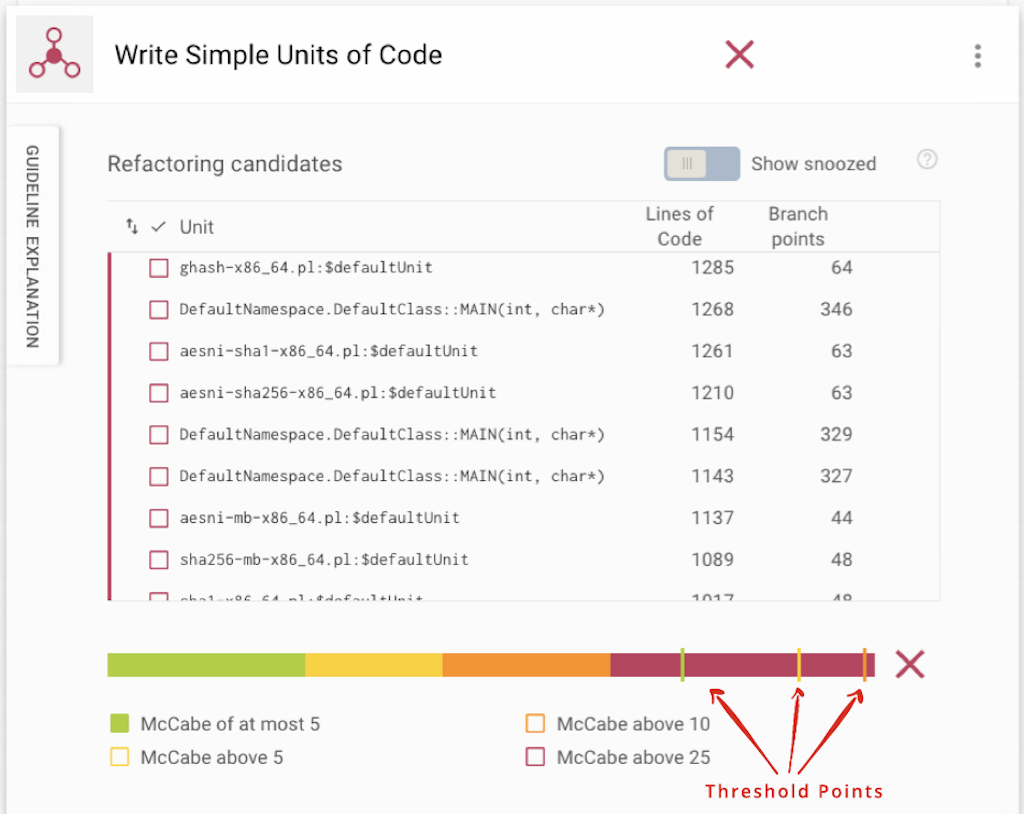
\includegraphics[width=0.8\textwidth]{Figures/bch_report.png}
  \caption{Maintainability report of OpenSSL's CVE-$2016$-$6304$ 
  vulnerability patch for the guideline \emph{Write Simple Units 
  of Code} provided by \emph{Better Code Hub}. This version of 
  OpenSSL does not comply with the guideline in the example since 
  the bars do not reach the threshold points. This example only 
  complies with $\sfrac{1}{10}$ guidelines (\emph{Write Clean 
  Code}).}
  \label{fig:bchrep}
\end{figure}

SIG defines \emph{Units} as the smallest groups of code that can be 
maintained and executed independently~\cite{Visser:2016:OREILLY} 
(e.g., methods and constructors in Java). One of the guidelines with 
which the project does not comply is the one presented in the report 
(cf. Figure~\ref{fig:bchrep}): \emph{Write Simple Units of Code}. BCH 
analyzes this guideline based on the McCabe 
Complexity~\cite{1702388} to calculate the number of branch points 
of a method. The bar at the bottom of the figure represents the top 
$30$ units that violate the guideline, sorted by severity. The 
different severities of violating the guideline are indicated using 
colors, and there is a legend to help interpret them. The green 
bar represents the number of compliant branch points per unit 
(\emph{at most $5$}), i.e., the number of units are compliant with 
ISO $25010$~\cite{iso:2011}. Yellow, orange, and red bars represent 
units that do not comply with medium (\emph{above $5$}), high 
(\emph{above $10$}) and very high (\emph{above $25$}) severity 
levels. In the bar, there are marks that pinpoint the compliance 
thresholds for each severity level. If the green mark is somewhere 
in the green bar, it is compliant with a low severity level.

Aiming to analyze the impact of security patches, we use BCH to compute 
the maintainability of two different versions of the project 
(cf. Figure~\ref{fig:commit}):

\begin{itemize}
	\item $v_{s-1}$, the version containing the security flaw, i.e., 
	before the patch (\emph{sha-p});
	\item $v_{s}$, the version free of the security flaw, i.e., 
	after the patch (\emph{sha});
\end{itemize}

\begin{figure}[h]
 	\centering 	
	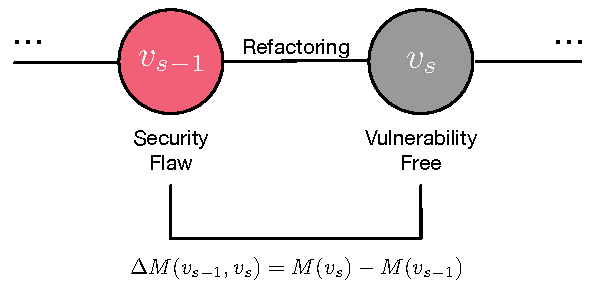
\includegraphics[width=0.5\linewidth]{Figures/commit.pdf}
 	\caption{Maintainability difference for security commits.}
	\label{fig:commit}
\end{figure}

Security patches can be performed through one commit (single-commit); 
several consecutive commits (multi-commits); or, commit(s) interleaved with more 
programming activities (floss-refactoring). Only $10.7\%$ of the data points 
of our dataset involve more than one commit, the other
$89.3\%$ of the cases are single-commit patches. To mitigate the impact of 
floss-refactorings, we extracted and manually inspected a random sample with 
$25\%$ of security patches from each dataset. From this sample, we identified 
$23$ floss-refactorings. Most floss-refactoring patches include many changes 
making it difficult to understand which parts involve the security patch. 
Although we suspect that more floss-refactorings may occur, we argue that 
they occur in a small portion of the data.

Due to BCH limitations, in particular, lack of language support 
and project size by BCH, $308$ data points were not analyzed and automatically 
disregarded from our study. After performing the BCH analysis and the 
maintainability calculations, we found the following 
limitations regarding two of BCH's guidelines:

1) For projects with large codebases, the results calculated for 
the \emph{Keep Your Codebase Small} guideline were way above the 
limit set by BCH ($20$ person-years). We suspect this threshold 
may not be well-calibrated, and hence biasing our results. Thus, 
we decided not to consider this guideline in our research. 

2) The 
\emph{Automated Tests} guideline was also not considered since the 
tool does not include two of the most important techniques to 
security testing: vulnerability scanning and penetration testing. 
Instead, it only integrates unit testing. 


The BCH tool does not compute the final score that our study needs 
to compare maintainability amongst different project versions. We 
follow previous work on measuring the impact of 
energy-oriented patches~\cite{8919169}. Cruz et al. ($2019$) 
proposed an equation to capture the distance between the current 
state of the project and the standard thresholds calculated by the 
BCH based on the insights provided in~\cite{Olivari:2018}. The 
equation provided in~\cite{8919169} considers that the size of 
project changes do not affect the maintainability, and that the 
distance to lower severity levels is less penalized than to the
thresholds in high severity levels.

% 	thresholds in high severity levels
% 	difference between two versions
% The equation considers the following:
% \begin{itemize}
% 	\item \textbf{Size of project changes does not affect the maintainability
% 	difference between two versions, $\Delta M (v_{s-1},v_{s}) = M(v_{s}) - M(v_{s-1})$.} We
% 	aim at evaluating security patterns occurring in different projects similarly.
% 	Thus, the derived metric uses the \textit{raw} number of lines of code rather
%   percentages for normalization purposes.
% 	\item \textbf{Distance to lower severity levels is less penalized than to the
% 	thresholds in high severity levels.} Severity level weights based on the
% 	severity level to count lines of code that violate maintainability guidelines.
% \end{itemize}


Given the violations for the BCH guidelines, the maintainability 
score is computed $M(v)$ as follows:

\begin{equation}
    M(v) = \sum_{g \in G}^{} M_{g}(v)
\end{equation}

\noindent
where $G$ is the group of maintainability guidelines from BCH
(Table~\ref{tab:guidelines}) and $v$ is the version of the software 
under evaluation. $M(v) < 0$ indicates that version $v$ is violating 
(some of) the guidelines, while $M(v) > 0$ indicates that version 
$v$ is following the BCH guidelines. The maintenance for the 
guideline $g$, $M_g$ for a given version of a project is computed as 
the summation of the compliance with the maintainability guideline 
for the given severity level (medium, high, and very high).
The compliance for a severity level is calculated based on previous 
work, which calculates the number of lines of code that comply and 
not comply with the guideline at a given severity 
level~\cite{8919169}. In our analysis, we compute the difference of 
maintainability between the security commit ($v_{s}$) and its parent 
commit ($v_{s-1}$), as illustrated in Figure~\ref{fig:commit}. Thus, 
we can determine which patches had a positive, negative, or null 
impact on the project maintainability. 

% The compliance $C$ for a given severity
% level $l$ is derived by:
%
% \begin{equation}\label{eq:3}
%     C(l) = LOC_{compliant}(l) - w(l) * LOC_{\neg compliant}(l)
% \end{equation}
%
% \noindent
% where $LOC_{compliant}(l)$ are the lines of code that comply with the guideline
% at the given severity level $l$, $LOC_{\neg compliant}(l)$ are the lines of code
% that do not comply with the guideline at the given severity level $l$ and $w(l)$
% is the weight factor to heighten the impact of non-compliant lines in comparison to
% compliant lines. Finally, the term $w(l)$ is calculated as follows:
%
% \begin{equation}
%     w(l) = \frac{1 - \theta(l)}{\theta(l)}
% \end{equation}
%
% \noindent
% where $\theta(l)$ is the threshold in percentage of the lines of code that are
% accepted to be non-compliant with the guideline for the severity level $l$. This
% is a standard value defined by BCH. In other words, the factor $w$ is used in
% Equation~\ref{eq:3} to highlight the lines of code that are not complying with
% the guideline. Then, we compute the difference of maintainability between the
% security commit ($v_{s}$) and its parent commit ($v_{s-1}$), as illustrated in
% Figure~\ref{fig:commit}.

\subsection{Statistical Validation}\label{sec:statsval}
%
To validate the maintainability differences in different groups of 
commits (e.g., baseline and security commits), we use the Paired 
Wilcoxon signed-rank test with the significance level $\alpha = 
0.05$~\cite{10.2307/3001968}. In other words, we test the null 
hypothesis that the maintainability difference between pairs of 
versions $v_{s-1}$, $v_s$ (i.e., before and after a security commit) 
come from the same distribution. Nevertheless, this test has a 
limitation: it does not consider the groups of commits with 
zero-difference maintainability. In $1959$, Pratt improved the 
test to solve this issue, making the test more robust. Thus, 
we use a version of the Wilcoxon test that 
incorporates the cases where maintainability is equal to 
zero~\cite{10.2307/2282543}. The Wilcoxon test requires a 
distribution size of at least $20$ instances. To understand the 
effect-size, as advocated by the Common-language effect 
sizes, we compute the mean difference, the median of 
the difference, and the percentage of cases that reduce 
maintainability~\cite{graw:1992}.
%

\section{Results \& Discussion}\label{sec:results}

This study evaluates a total of $969$ security patches and 
$969$ regular changes 
from $260$ distinct open-source projects. 
This section 
reports and discusses the results for each research question.
%

\textit{\textbf{RQ1: What is the impact of security patches on the
maintainability of open-source software?}} In \emph{RQ1}, we 
report and discuss the impact of patches on open-source software 
maintainability under four groups: guideline, overall score, 
severity and programming language.

\textbf{Guideline/Metric:} Each patch performs a set of changes
on the software's source code. These changes may have a 
different impact on the guidelines/metrics used to measure software 
maintainability. Figure~\ref{fig:guidelines} shows the impact of 
security patches on each guideline individually and the average 
impact on all guidelines together ($M(v)$). Under each guideline, it 
is stated the metric used for the calculations. For instance, for the 
\emph{Write Short Units of Code} guideline, the metric used is 
\emph{Unit Size}. Table~\ref{tab:guidelines} describes in more 
detail the metrics behind the guidelines. For each type of 
guideline, a swarm plot is presented to show the variability/dispersion 
of the results alongside the number of absolute and 
relative cases of each impact. Next to each type of guideline, it is 
presented the mean ($\overline{x}$) and median (M) of the 
maintainability difference and the p-value resulting from the Paired 
Wilcoxon signed-rank test. $M(v)$ is not a guideline but rather the 
average impact of all guidelines. Each point of the plot represents 
the impact of a security patch on software maintainability. Red 
means the impact was negative, i.e., the patch harmed 
maintainability. Yellow means the patch did not have any kind of 
impact on maintainability. Green means the impact was positive, i.e., 
the patch improved software maintainability.

 \begin{figure}[htp]
     \begin{adjustwidth}{-1cm}{-1cm}  
  	\centering
  	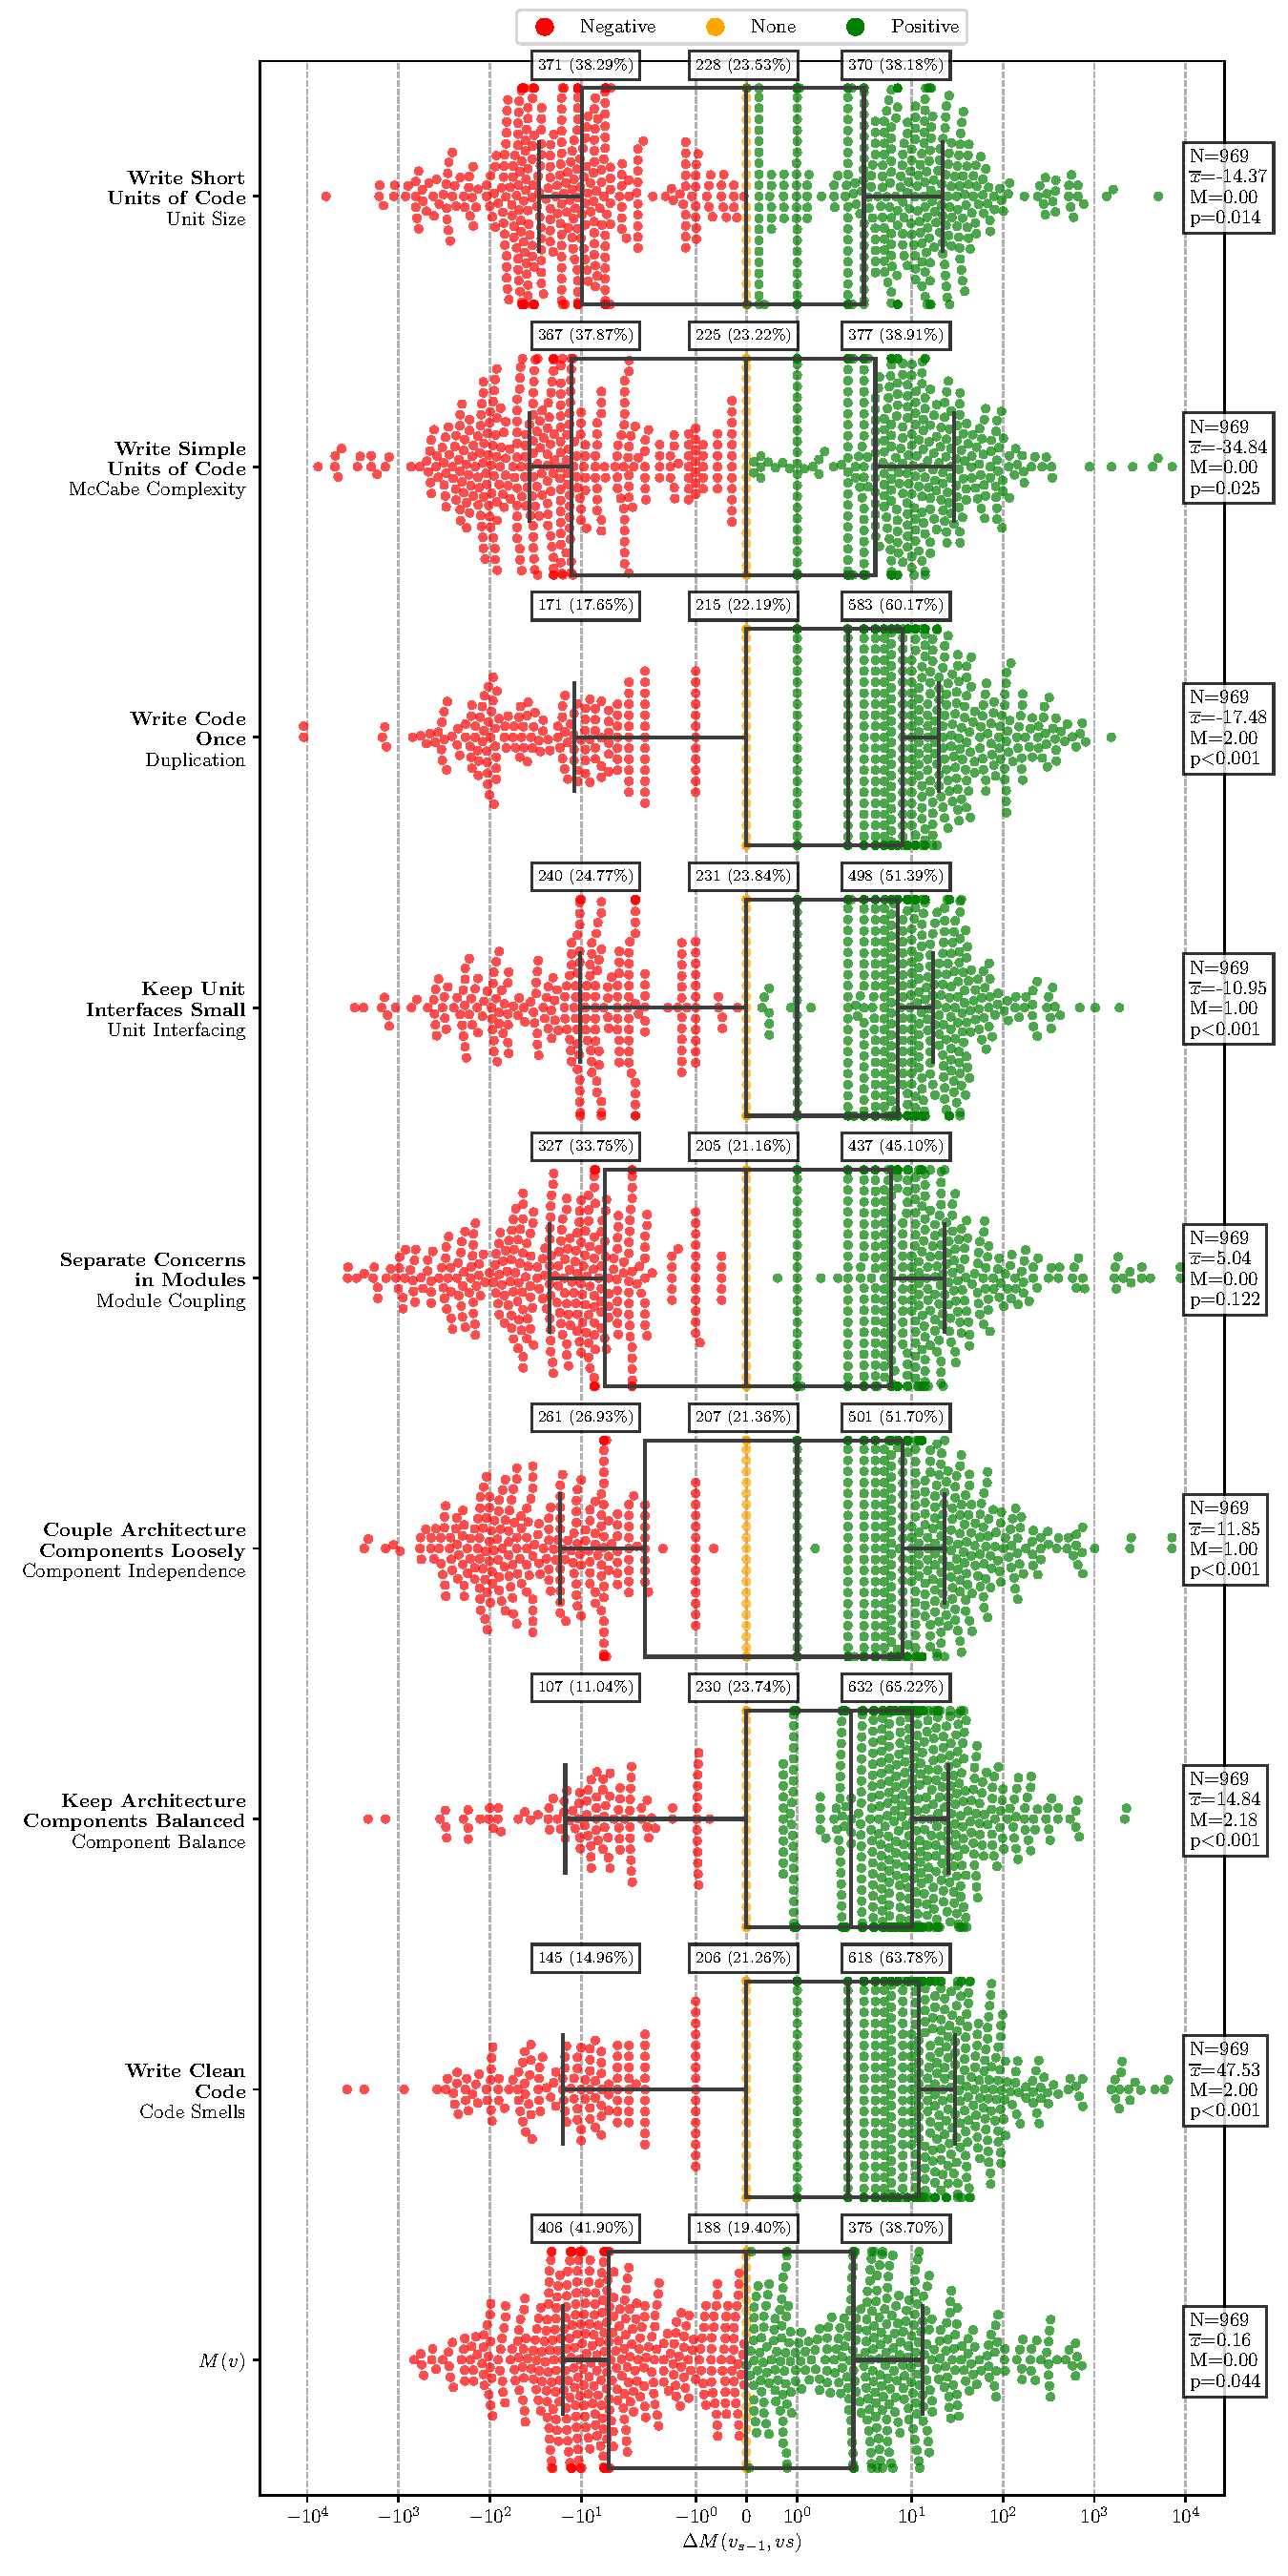
\includegraphics[width=0.9\textwidth]{Figures/main_per_guideline.pdf}
    \end{adjustwidth}
	
  	\caption{Impact of the security patches per guideline and overall mean, $M(v)$. 
    Each point of the plot represents the impact of a security patch on software 
    maintainability. Red means the impact was negative, i.e., the patch 
    harmed maintainability. Yellow means the patch did not have any 
    kind of impact on maintainability. Green means the impact was 
    positive, i.e., the patch improve software maintainability. For instance, in the 
    \emph{Write Short Units of Code} guideline, $38.29\%$ of 
    security patches harmed software maintainability; $23.53\%$ of 
    security patches had no impact on maintainability; and, 
    $38.18\%$ of security patches improved software maintainability.}
 	\label{fig:guidelines}	
 \end{figure}
 
 \begin{figure}[htp]
  	\centering 	 	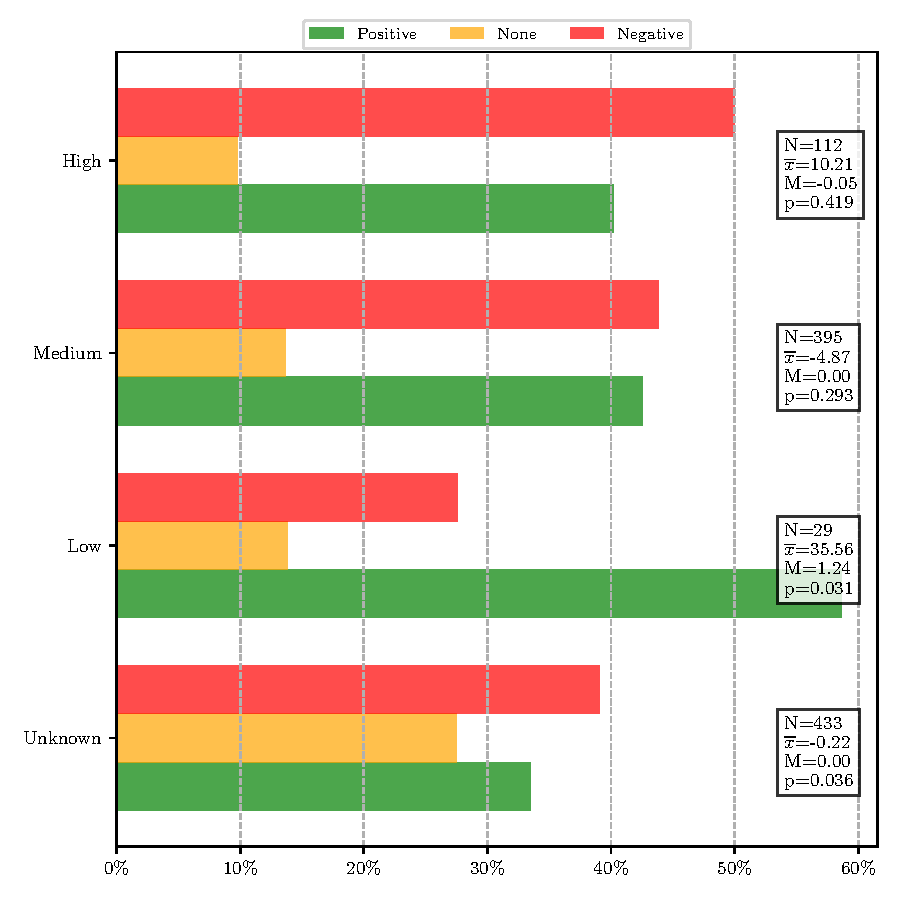
\includegraphics[width=0.65\textwidth]{Figures/main_per_severity.pdf}
  	\caption{Maintainability difference by vulnerability severity.}
 	\label{fig:severity}
 \end{figure}

 Regarding the impact of security patches per guideline, we 
 observe that $38.7\%$ of the security patches have positive impact
 on software maintainability. However, we also 
 see that patching vulnerabilities have a very significant number of 
 negative cases per guideline---between $10\%$ and $40\%$. 
 \emph{Write Short Units of Code} ($38.3\%$), \emph{Write Simple 
 Units of Code} ($37.9\%$), and \emph{Separate Concerns in Modules} 
 ($33.8\%$) seem to be the most negatively affected guidelines. This 
 may imply that developers, when patching vulnerabilities, have a hard 
 time designing/implementing solutions that continue to respect the 
 limit bounds of branch points and function/module sizes that are 
 recommended by coding practices. Still, on respecting bound limits, 
 developers also seem not to consider the limit of $4$ parameters per 
 function for the \emph{Keep Unit Interfaces Small} guideline 
 required by BCH, in $24.8\%$ of the cases. This guideline is usually
 violated when the patch requires to input new information to a 
 function/class, and developers struggle to use the \emph{Introduce 
 Parameter Object} patch pattern. Results do not provide statistical 
 significance to the \emph{Separate Concerns in Modules} guideline, 
 i.e., results should be read carefully.

Software architecture is also affected while patching 
vulnerabilities. Both \emph{Couple Architecture Component Loosely} 
and \emph{Keep Architecture Components Balanced} guidelines suffer a 
negative impact of $26.9\%$ and $11.0\%$, respectively. Component 
independence and balance are important to make it easier to find the 
source code that developers want to patch/improve and to understand 
how the high-level components interact with others. However, results 
may imply that developers forget to use techniques such as 
encapsulation to hide implementation details and make the system 
more modular.

The \emph{Write Code Once} guideline results show that duplicated 
code increased in $17.7\%$ ($171$/$969$) of the patches. Software systems 
typically have $9\%$-$17\%$ of cloned code~\cite{5773403}. Previous work showed a correlation between code smells and code
duplication~\cite{7476787} which may also be reflected in the 
\emph{Write Clean Code} guideline results. BCH reported new code 
smells for $15.0\%$ ($145$/$969$) of the patches, which according to previous work, 
may be the source of new software vulnerabilities~\cite{8819456,10.1145/3133956.3134072}
capable of harming the market value and economy of companies~\cite{4267025}.
Developers should never reuse code by copying and pasting 
existing code fragments. Instead, they should create a method and call 
it every time needed. The \emph{Extract Method} refactoring 
technique solves many duplication problems. This makes spotting and solving 
the issue faster because you only need to fix the method used
instead of locating and fixing the issue multiple times.
Clone detection tools can also help in locating the issues.

\textbf{Overall Score ($M(v)$):} 
Although overall patching vulnerabilities has a less negative impact
on software maintainability guidelines, this is not reflected in the 
average impact of all guidelines ($M(v)$) as we can see in 
Figure~\ref{fig:guidelines}. Remember that each point of the plot 
represents the impact of a security patch on software 
maintainability. Red means the impact was negative, i.e., the patch 
harmed maintainability. Yellow means the patch did not have any kind of 
impact on maintainability. Green means the impact was positive, i.e., the patch improved software maintainability.
The $M(v)$ plot shows that $406$ ($41.9\%$) cases have a negative impact 
on software maintainability. While $188$ ($19.4\%$) cases 
have no impact at all, and $375$ ($38.7\%$) have a positive impact on 
software maintainability. The larger number of negative cases may be 
explained by guidelines with higher concentrations of negative 
cases with higher amplitudes, such as \emph{Write Short Units of 
Code}, \emph{Write Simple Units of Code} and \emph{Separate Concerns 
in Modules}---more red points on the left, being $0$ the reference point.
The resulting p-value of the Paired Wilcoxon signed-rank test for $M(v)$ 
is $0.044$ (cf. Figure~\ref{fig:guidelines}). Since the p-value is 
below the significance level of $0.05$, we argue that security patches 
may have a negative impact on the maintainability of open-source software.


\textbf{Severity:} Some of the vulnerabilities are identified with 
\emph{Common Vulnerabilities and Exposure} (CVE) entries. We 
leveraged the \emph{National Vulnerability Database} (NVD) website 
to collect their severity levels. In total, we retrieved severity 
scores for $536$ vulnerabilities: $112$ \emph{High}, $395$ 
\emph{Medium} and $29$ \emph{Low}. Figure~\ref{fig:severity} 
presents the impact of security patches per severity level on the 
maintainability of open-source software. We observe that patches for 
\emph{High} ($50.0\%$) and \emph{Medium} ($43.8\%$) severity 
vulnerabilities hinder more the maintainability of software than 
\emph{Low} ($27.6\%$) severity vulnerabilities. Again, patches have 
a considerable negative impact on software maintainability---between 
$20\%$ and $50\%$. Statistical significance was retrieved only for 
\emph{Low} severity vulnerabilities, i.e., \emph{Low} severity 
vulnerabilities may have more cases where software maintainability was improved than the 
other severity levels. However, results should not be disregarded 
because they somehow confirm the 
assumption that higher severity vulnerabilities patches may have a 
more negative impact on maintainability, i.e., high/medium 
severity vulnerabilities may need more attention than low severity while 
patching.


\begin{figure}[htp]
  \centering
  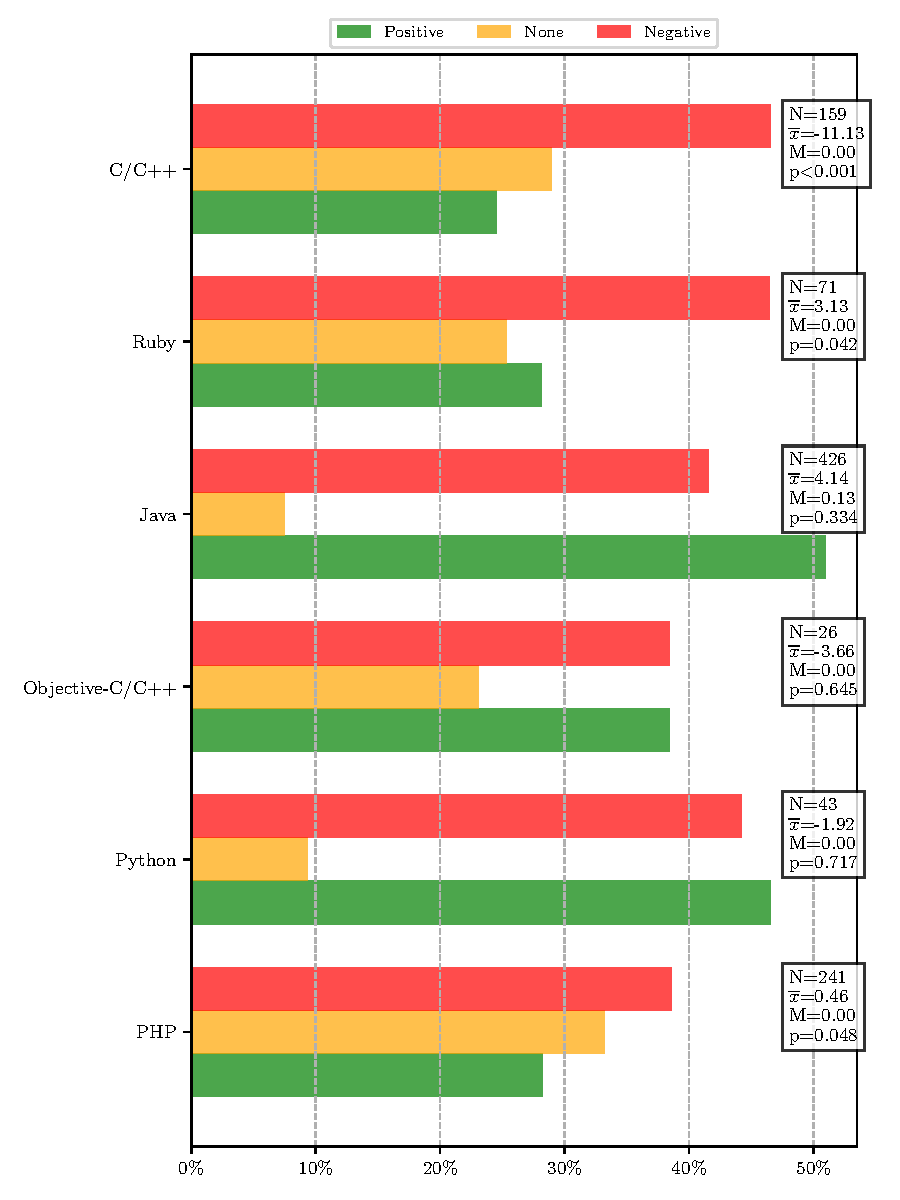
\includegraphics[width=0.6\textwidth]{Figures/main_per_language.pdf}
  \caption{Maintainability difference by programming language.}
  \label{fig:lang_main}    
\end{figure}

% TODO
% \begin{figure*}[htp]
%   \centering
%   \subfigure[Maintainability difference by first-level weaknesses from the 
%   \textit{Research Concepts} list on Common Weakness Enumeration (CWE)]{
%   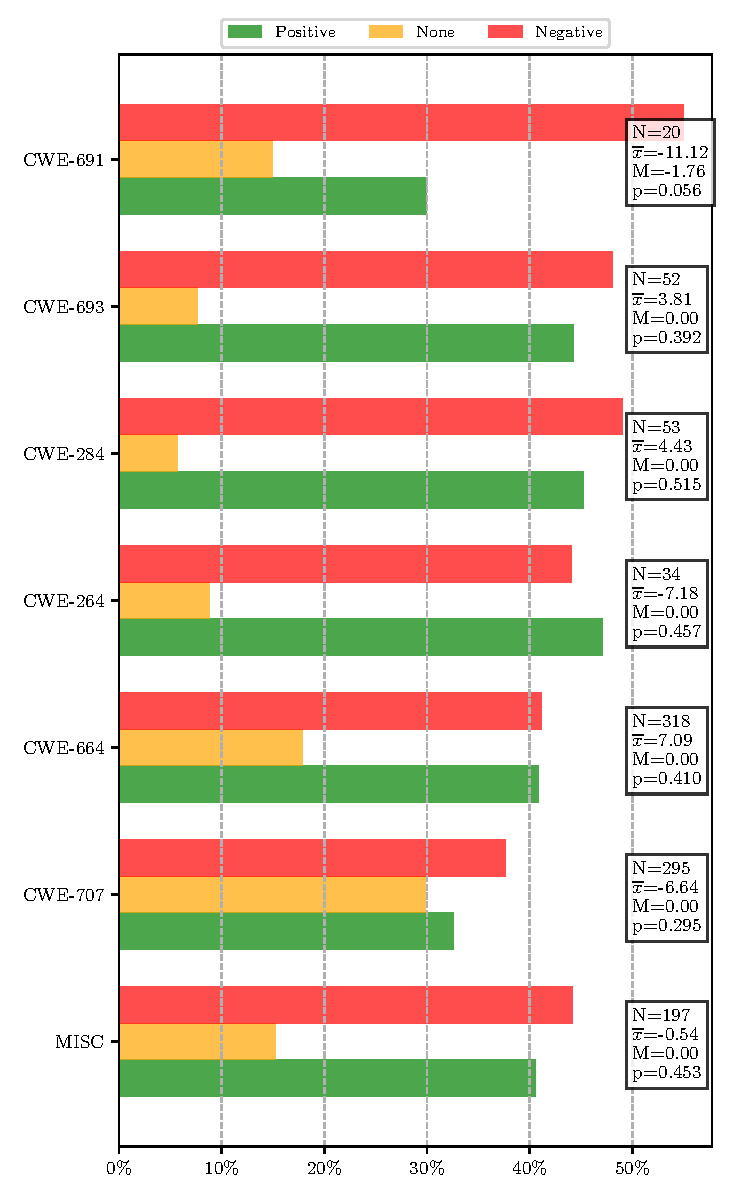
\includegraphics[scale=0.4]{Figures/main_per_cwe.pdf}}\quad\quad
%   \subfigure[Maintainability difference by sub-weaknesses of the 
%   \textit{Improper Neutralization} Weakness (CWE-707)]{
%   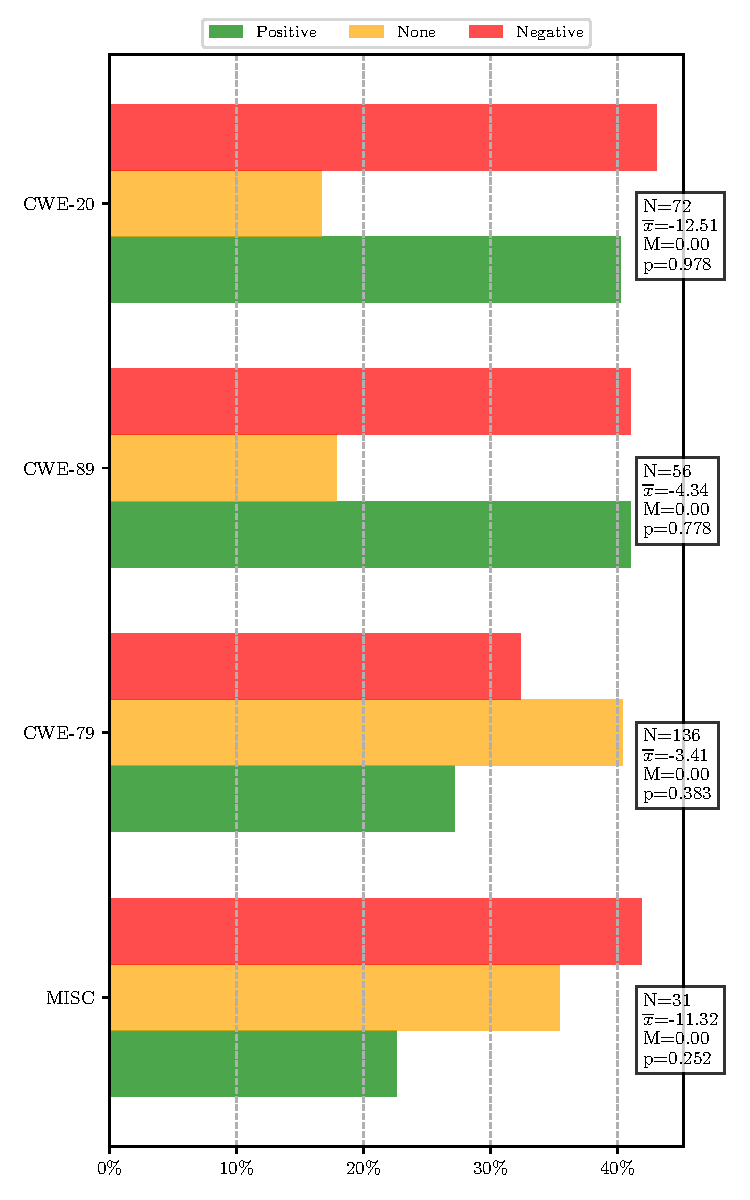
\includegraphics[scale=0.4]{Figures/main_per_cwe_spec_707.pdf}}\quad\quad
%   \subfigure[Maintainability difference by sub-weaknesses of the 
% 	\textit{Improper Control of a Resource Through its Lifetime} Weakness (CWE-664)]{
% 	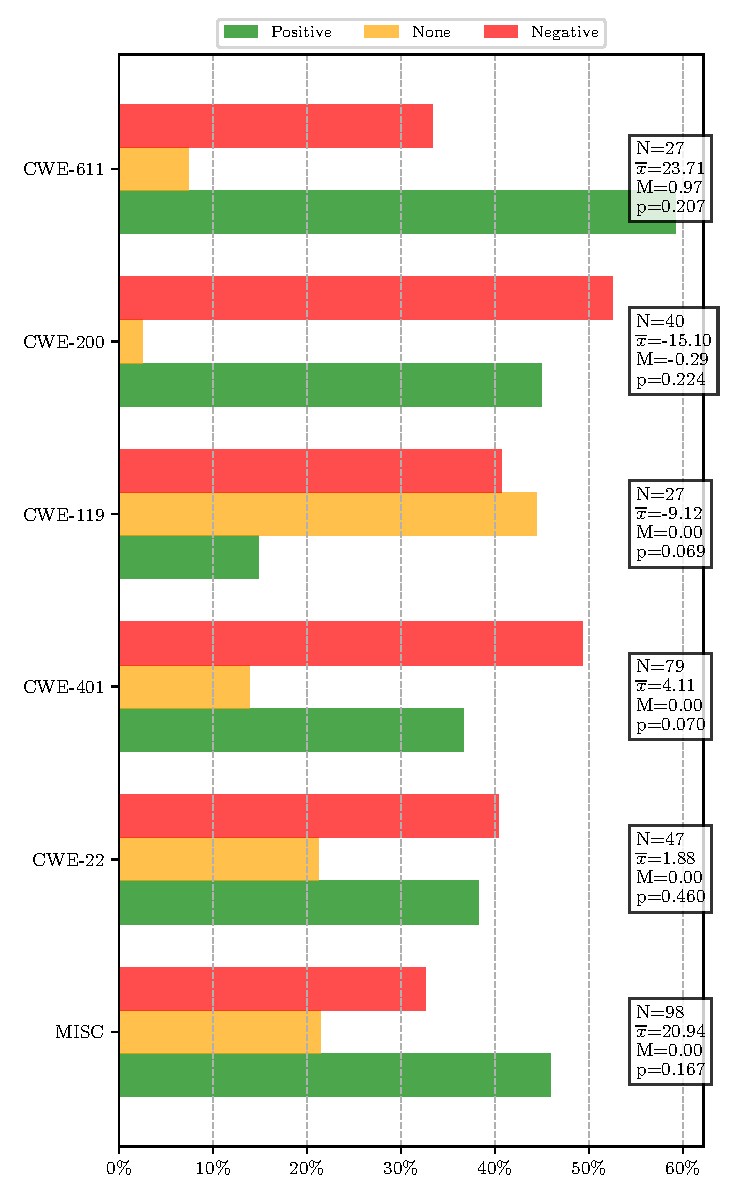
\includegraphics[scale=0.4]{Figures/main_per_cwe_spec_664.pdf}}
%     \caption{Maintainability difference per weakness.}
% 	\label{fig:pat}
% \end{figure*}

\textbf{Programming Language:} The impact on software maintainability per programming 
language was also analyzed (Figure~\ref{fig:lang_main}). We restrict 
this analysis to programming languages with at least $20$ data points, as this 
is a requirement for the hypothesis tests. Thus, we compare the results for 
\texttt{C/C++}, \texttt{Ruby}, \texttt{Java}, \texttt{Objective C/C++}, 
\texttt{Python} and \texttt{PHP}, leaving \texttt{Groovy} out of the analysis.
\texttt{C/C++}, \texttt{Ruby} and 
\texttt{PHP} are the programming languages with worse 
impact on maintainability, i.e., with the highest number of negative cases ($46.5\%$, $46.5\%$ 
and $38.6\%$, respectively). \texttt{Java} and \texttt{Python} 
seem to be less affected by patching, i.e., integrating a larger amount of cases with positive 
impact on maintainability ($50.9\%$ and $46.5\%$, respectively). But overall 
languages have a considerable amount of cases that negatively impact maintainability---between $35\%$ to $50\%$---which 
confirms the need for better/more secure programming languages. 
Statistical significance was only retrieved for the \texttt{C/C++} 
($p = 2.24$x$10^{-05}$), \texttt{Ruby} ($p = 0.041$) and \texttt{PHP} 
($p = 0.048$) languages. Yet, data reports very interesting hints on the impact 
of programming languages on security patches.

We expected the negative impact for programming languages on
maintainability to be more severe, as arguably, poor design of programming
languages for security and the lack of best practices application by developers lead to more buggy/vulnerable
code~\cite{Ray:2017:LSP:3144574.3126905,2019arXiv190110220B}. However,
Figure~\ref{fig:lang_main} shows that only \emph{C/C++} and \emph{Ruby} have 
a significant negative impact approximate to $50\%$ on 
maintainability. We suspect that these values are
the result of project contributions policies (e.g., coding standards). In our dataset, 
$9$/$10$ projects with more contributors follow strict contribution 
policies for code standards. 


\textbf{Summary:} Results show that developers may have a
hard time following the guidelines and, consequently, hinder
software maintainability while patching vulnerabilities; and that different levels of
attention should be paid to each guideline. For instance,
\emph{Write Simple Units of Code} and \emph{Write Short Units of Code}
guidelines are the most affected ones. No statistical significance was observed
for \emph{Separate Concerns in Modules}.
As shown in Figure~\ref{fig:guidelines}, there is statistical significance ($p=0.044 < 0.05$) 
to support our findings: \textbf{security patches
may have a negative impact on the maintainability of open-source software}. Therefore, tools 
such as BCH should be integrated into the CI/CD pipelines
to help developers evaluate the risk of patches of hindering software maintainability---alongside
Pull Requests/Code Reviews. Different severity
vulnerabilities may need different levels of attention---high/medium 
vulnerabilities need more attention (cf. Figure~\ref{fig:severity}). However, 
statistical significance was only observed for low severity vulnerabilities. Better 
and more secure programming languages are needed. We observed statistical 
significance for \emph{C/C++}, \emph{Ruby} and \emph{PHP} that support that 
security patches in those languages may hinder software maintainability (cf. Figure~\ref{fig:lang_main}).
%

\textit{\textbf{RQ2: Which weaknesses are more likely to
affect open-source software maintainability?}}
In \emph{RQ2}, we report/discuss the impact of security patches on
software maintainability per weakness (CWE). We use the weakness definition
and taxonomy proposed by the \emph{Common Weakness Enumeration} (cf. Section~\ref{sec:motivation}).
Figure~\ref{fig:pat} shows three different charts. Figure \emph{\ref{fig:pat}-a}, presents
the impact of the $969$ patches grouped by the first level weaknesses from
the \emph{Research Concepts}\footnote{Research Concepts 
 is a tree-view provided by the Common Weakness Enumeration (CWE) website 
 that intends to facilitate research into weaknesses. It is organized 
 according to 
 abstractions of behaviors instead of how they can be detected, 
 their usual location in code, and when they are introduced in the 
 development life cycle. The list is available here: \url{https://cwe.mitre.org/data/definitions/1000.html}
} list. While the Figures \emph{\ref{fig:pat}-b} and
\emph{\ref{fig:pat}-c} present the impact on maintainability for lower levels of 
weaknesses for the most prevalent weaknesses in Figure \emph{\ref{fig:pat}-a}:
\emph{Improper Neutralization} (CWE-707) 
and \emph{Improper Control of a Resource 
Through its Lifetime} (CWE-664), respectively.

In Figure~\ref{fig:pat}-\emph{a}, there is no clear evidence of the impact on 
maintainability per weakness. Yet, it is important to note that
overall there is a very considerable number of cases that hinder
maintainability---between $30\%$ and $60\%$. The CWE-707 and CWE-664 
weaknesses integrate the higher number of cases compared to the remaining 
ones: $295$ ($30.4\%$) data points and $318$ ($32.8\%$) data points, respectively. 
Thus, we present an analysis of their sub-weaknesses on 
Figure~\ref{fig:pat}-\emph{b} and Figure~\ref{fig:pat}-\emph{c}, respectively. 

Results shows that patching vulnerabilities may hinder 
the maintainability of open-source software in $4$ different sub-weaknesses: 
\emph{Improper Input Validation (CWE-20)}, \emph{Information Exposure 
(CWE-200)}, \emph{Missing Release of Memory after Effective 
Lifetime (CWE-401)} and \emph{Path Traversal (CWE-22)}. Results also show that 
software maintainability is less negatively impacted when patching 
\emph{Improper Restriction of XML External Entity Reference (CWE-611)}.  

The impact of a patch depends on its complexity, i.e., if the patch
adds complexity to the code base, it is probably affecting the software
maintainability. \emph{Cross-Site Scripting (CWE-79)} and 
\emph{Improper Restriction of Operations within the Bounds of 
a Memory Buffer (CWE-119)} patches endure more
cases with no impact on the open-source software maintainability. \emph{SQL Injection
(CWE-89)} patches equally hinder and improve software maintainability.
These patches usually follow the same complexity as the CWE-79 patches.
However, the three weaknesses have a considerable amount of cases that hinder
the software maintainability---$32.4\%$, $40.7\%$ and, $41.1\%$, respectively---which
should not be happening. Typically, CWE-79 vulnerabilities do not need extra lines 
to be fixed, as shown in Listing~\ref{lst:fix}---one simple 
\texttt{escape} function patches the issue. On the same type of fix,
CWE-199 vulnerabilities may also be fixed without adding new source code
(e.g., replacing the \texttt{strncpy} function with a more secure one 
\texttt{strlcpy} that checks if the buffer is null-terminated). However,
some buffer overflows may be harder to fix and lead to more complex 
solutions (e.g., 
CVE-$2016$-$0799$\footnote{CVE-$2016$-$0799$ patch details available at 
\url{https://github.com/openssl/openssl/commit/9cb177301fdab492e4cfef376b28339afe3ef663}
(Accessed on \today{})}). 
As CWE-199 weaknesses, \emph{Missing Release of Memory after Effective 
Lifetime (CWE-401)} can also be the cause of Denial-of-Service attacks and difficult to 
patch since it usually requires adding complexity to the program (cf. Section~\ref{sec:motivation}). 

\textbf{Summary:}
Although results did not yield statistical significance, we show preliminary evidence that 
researchers and developers ought to pay more attention to maintainability when fixing the 
following types of weaknesses: \emph{Improper Input Validation (CWE-20)}, \emph{Information Exposure
(CWE-200)}, \emph{Missing Release of Memory after Effective
Lifetime (CWE-401)} and \emph{Path Traversal (CWE-22)}.


\textit{\textbf{RQ3: What is the impact of security patches versus regular 
changes on the maintainability of open-source software?}}
The impact of security and regular changes on software maintainability 
is presented in Figure~\ref{fig:secvsreg}. In this section, 
we present a comparison of security patches with 
two different baselines of regular changes: 
\emph{size-baseline}, a dataset of  
random regular changes with the same size as security 
patches---we argue that comparing changes with considerable different 
sizes may be unfair; and, \emph{random-baseline},
a dataset of random regular changes. 

Our hypothesis is
that \emph{security patches hinder more software maintainability 
than regular changes}. 
We have seen, previously, a deterioration in software maintainability 
when patching vulnerabilities: $41.9\%$ ($406$) of patches suffered a 
negative impact, $38.7\%$ ($375$) of patches remained the same, and $19.4\%$ 
($188$) of patches increased software maintainability. For regular changes,
when considering the size of the changes (\emph{size-basline}),
we observe that the maintainability decreases in $27.0\%$ ($262$) 
and increases in $30.5\%$ ($295$) of the cases. But in contrast to 
security patches, the maintainability of regular changes remains the 
same in $42.5\%$ ($412$) of the cases, i.e., performing regular
changes has a more positive impact than negative on  
maintainability. However, no statistical significance was 
obtained. Regular changes (\emph{random-baseline}), with no size 
restrictions, are less prone to hinder software maintainability than 
security changes. About $34.4\%$ ($333$) of the regular changes hinder 
software maintainability---less than in the security patches. For the \emph{random-baseline}, 
statistical significance was retrieved ($p = 5.34$x$10^{-8}$).


\begin{figure}[htp]
  \centering
  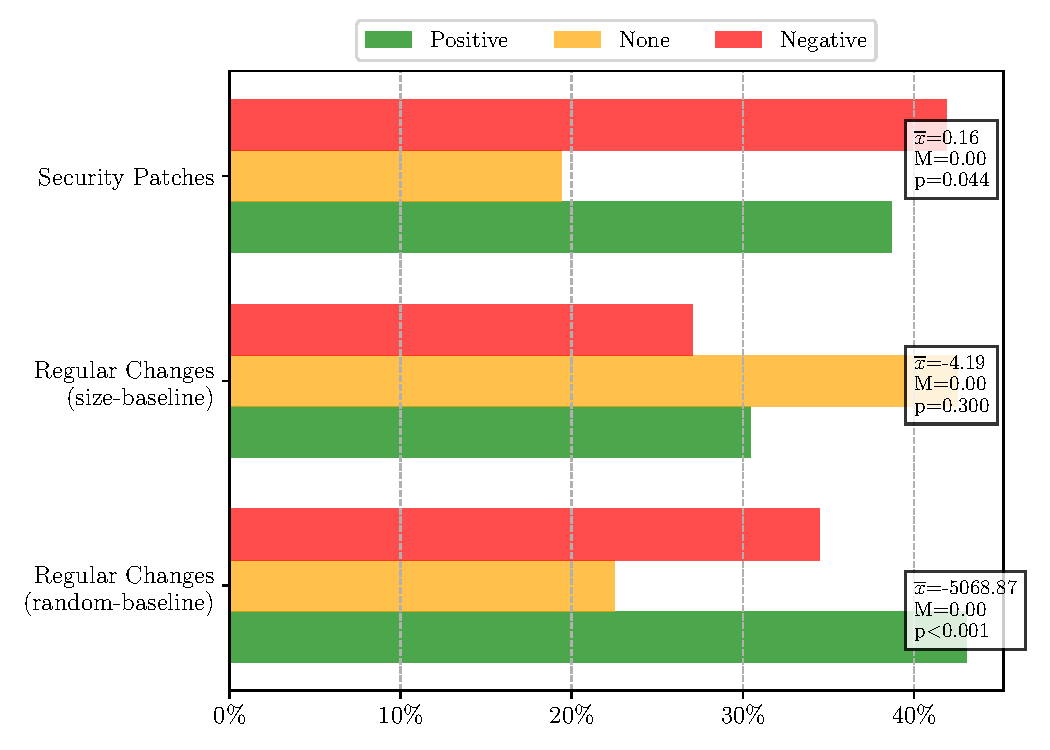
\includegraphics[width=0.8\textwidth]{Figures/baseline.pdf}
  \caption{Maintainability difference of security patches versus regular changes.}
  \label{fig:secvsreg}    
\end{figure}

Overall, the results for both baselines show that regular 
changes are less prone to hinder the software 
maintainability of open-source software.   
However, the \emph{size-baseline} integrates a larger 
number of cases with no impact on software maintainability. 
We manually inspected a total of $25$ cases from
that distribution of regular changes with no impact on maintainability, 
and found that identifying regular changes with the same 
size as the security-related commit is limiting the type of regular 
commits being randomly chosen: input 
patches, variables or functions, type conversion (i.e., changes
with no impact on the software metrics analyzed by BCH).
We presume that this phenomenon lead
to the significant number of cases where there is no impact
on the software maintainability. On the other hand, 
identifying regular changes without any restrictions (\emph{random-baseline})
shows that regular changes have a less negative impact 
on software maintainability when compared to security patches
and that special attention should be given to security patches.

\textbf{Summary:} Security-related commits are observed to harm software 
maintainability, while regular changes are less prone to harm software maintainability.
Thus, we urge the importance of adopting maintainability practices while 
applying security patches.



\section{Study Implications}\label{sec:implications}
%
Our results show evidence that developers may have to reduce maintainability for the 
sake of security. We argue that developers should be able to patch and produce 
secure code without hindering the maintainability of their projects. But there are 
still concerns that need to be addressed and that this study brings awareness for:
%

\textit{\textbf{Follow Best Practices:}} Developers are not 
paying attention to some quality aspects of their solutions/patches, 
as seen in Figure~\ref{fig:guidelines}, ending up harming 
software maintainability. We argue that developers
should design and implement solutions that respect the 
limit bounds of branch points and function/module sizes that are 
recommended by best practices to avoid increasing the 
size, complexity, and dependencies of their patches.
Developers should also keep function parameters below 
the recommended limit. It helps keep unit interfaces small 
and easy to use and understand.
Patterns such as \emph{Introduce Parameter Object} are useful 
to send information to a new function/class through an object
and keep the number of parameters small and the information well-organized.

Security patches also harm the maintenance of software architecture. Maintaining the components independence and balance 
is important to make it easier to find the source code that 
developers want to patch/improve and to better understand
how the high-level components interact with others. Applying 
\emph{encapsulation} to hide implementation details and make the system 
more modular is a step forward not to hinder software architecture maintainability.

According to previous research, there is a correlation between 
code duplication and code smells~\cite{7476787}---duplicates are a source 
of regression bugs. BCH reports new code smells
for $15\%$ of the patches under study which supports previous research---$34\%$ of security patches 
introduce new problems~\cite{8819456,10.1145/3133956.3134072}. 
Developers should never reuse code by copying and pasting 
existing code fragments. Instead, they should create a method and call 
it every time needed. The \emph{Extract Method} refactoring 
technique solves many duplication problems. This makes spotting and 
solving the issue faster because you only need to fix one method instead
of multiple vulnerabilities. Clone detection tools such as CPD can help 
on locating duplicates.

\textit{\textbf{Prioritize High and Medium Severity:}} Previous research 
exhibits proof that developers prioritize
higher impact vulnerabilities~\cite{10.1145/3133956.3134072}.
Our study shows that vulnerabilities of high and
medium severity should be prioritized in software maintainability tasks.

\textit{\textbf{Some Types of Vulnerabilities Need More Attention:}} 
Our study attempted to shed light on the impact of different types of vulnerabilities on software maintainability.
Overall, all the CWEs under study present a negative impact
over $30\%$ on software maintainability. 
\emph{Cross-Site Scripting} (CWE-79) and \emph{Improper 
Restriction of Operations within the Bounds of a Memory Buffer} (CWE-119) 
are less prone to have an impact on open-source software maintainability.
Developers should pay special attention to \emph{Improper Input Validation} (CWE-20), 
\emph{Information Exposure} (CWE-200), \emph{Missing Release of Memory after Effective Lifetime} 
(CWE-401) and \emph{Path Traversal} (CWE-22). However, 
more research should be performed to better understand the impact of each guideline on each CWE.

\textit{\textbf{Tools for Patch Risk Assessment Wanted:}}
  Design debt of one guideline can lead to severe impacts on the 
  software quality~\cite{10.1145/1985362.1985366}. Some software 
  producers consider security as a first-class citizen while others do not. As 
  mentioned in previous work, security is critical and should be considered as a 
  default feature~\cite{10.1145/2489828.2489830,kurilova2014wyvern,mcgraw2004software}. 
  However, the lack of experts and awareness of developers for security while 
  producing/patching software leads companies to ship low-quality software. 
  Providing automated tools to developers to assess the risk of their patches is 
  essential to help companies shipping software of higher quality. 
  Bryan O'Sullivan, VP of Engineering at Facebook, advocated for new computer science
  risk models to detect vulnerabilities in scale and predict the level of security 
  of the software under production in his talk ```Challenges in Making Software Work at Scale''' at FaceTAV’20.

  Tools like Better Code Hub can complement static analysis (e.g., 
  SonarQube, Codacy, ESLint, Infer, and more) to provide more informatio

\section{Threats to Validity}\label{sec:threats}
%
This section presents the potential threats to the validity of this study.
%

\textit{\textbf{Construct Validity:}} The formula to calculate the 
maintainability value ($M(v)$) was inferred based 
on the BCH's reports. The high amount of different projects and backgrounds 
may require other maintainability standards. However, BCH does use a 
representative benchmark of closed and open-source software projects to 
compute the thresholds for each maintainability guideline~\cite{Visser:2016:OREILLY,baggen2012}.
Maintainability is computed as the mean of all guidelines. Different software versions 
(vulnerable/fixed) of one vulnerability may have the same overall score
and still be affected by different guidelines. Therefore, we provide
an analysis per guideline, and our results are all available on GitHub for future reproductions and deeper analysis. 

\textit{\textbf{Internal Validity:}} The security patches dataset provided by previous
work~\cite{Reis:2017:IJSSE} was collected based on the messages of GitHub
commits produced by project developers to classify the changes performed while 
patching vulnerabilities. This approach discards patches that were
not explicit in commits messages. We assume that patches were performed using 
a single commit or several sequentially. The perspective that a 
developer may quickly perform a patch and later proceed to the refactor is 
not considered. We assume that all patches were only performed once. Depending 
on the impact of the vulnerability in the system, some vulnerabilities may have 
more urgency to be patched than others. For instance, a vulnerability performing a Denial-of-Service attack
that usually brings entire systems down may be more urgent to patch than a 
cross-site scripting vulnerability which generally does not have an impact
on the execution of the system but rather on the data accessibility.
We manually inspected $25.1\%$ of the security patches looking for floss-refactorings---$122$ from each dataset. We did 
find $23$ cases we argue to be floss-refactorings and toss them
to minimize the impact of this threat.

Baseline commits are retrieved randomly from 
the same project as the security patch.
This approach softens the differences
that may result from the characteristics of each project. However,
maintainability may still be affected by the developers' experience, coding
style, and software contribution policies which are not evaluated in this study.
Furthermore, this evaluation considers that $969$ regular commits---any kind
of commit---are enough to
alleviate random irregularities in the maintainability differences of the
baseline. 
%

\textit{\textbf{External Validity:}} The BCH tool uses private and open-source 
data to determine the thresholds for each guideline. We only analyze patches of open-source software.
Thus, our findings may not extend to private/non-open source software. 
Different programming languages may require different coding practices to address 
software safety. The dataset comprises more commits in Java, i.e., the dataset 
may not be representative of the population regarding programming languages. 
For both datasets, manual validation of the message of the commits was performed. 
Only commits in English were considered. Thus, our approach does not consider 
patches in any other language but English.

\section{Related Work}\label{sec:rw}

Many studies have investigated the relationship between patches and
software quality. Previous work focused on object-oriented metrics has evaluated the
impact of patches and exhibited proof that quantifying the
impact of patches on maintainability may help to choose the appropriate
patch type~\cite{1167822}. In contrast to this work, Hegedus et
al.~\cite{HEGEDUS2018313} did not select particular metrics to assess the effect
of patches. Instead, statistical tests were used to find the metrics that
have the potential to change significantly after patches. 

Researchers
performed a large-scale empirical study to understand the characteristics of security patches
and their differences against bug fixes~\cite{10.1145/3133956.3134072}.
The main findings were that security patches are smaller and less complex than bug 
fixes and are usually performed at the function level. Our study compares
the impact of security patches on software maintainability with the impact 
of regular changes.

Studying the evolution 
of maintainability issues during the development of Android apps, Malavolta et al. ($2018$)~\cite{8530041}
discovered that maintainability decreases over time. Palomba et al.
($2018$)~\cite{Palomba:2018:DIM:3231288.3231337} exhibits proof that code smells
should be carefully monitored by programmers since there is a high correlation
between maintainability aspects and proneness to changes/faults. In 2019, Cruz et 
al.~\cite{8919169} proposed a formula to calculate maintainability based on the 
BCH's guidelines and measured the impact of energy-oriented fixes 
on software maintainability. Recent work
proposed a new maintainability model to measure fine-grained code changes by 
adapting/extending the BCH model~\cite{8785997}.
Our work uses the same base model (SIG-MM) but considers a broader set of guidelines. 
Moreover, we solely focus on evaluating the impact of security patches on software maintainability.

Researchers investigated the relationship between design patterns and
maintainability~\cite{10.1007/978-3-642-35267-6-18}. However, other studies 
show that the use of design patterns may introduce maintainability issues into
software~\cite{4493325}. Yskout et. al did not detect if the usage of design 
patterns has a positive impact but concluded that developers prefer to work with 
the support of security patterns~\cite{8077802}. The present work studies how 
security weaknesses influence maintainability for open-source software.

There are studies that investigated the impact of programming languages on software
quality~\cite{Ray:2014:LSS:2635868.2635922,Ray:2017:LSP:3144574.3126905}. The first
one shows that some programming languages are more buggy-prone than others. However,
the authors of the second one could not reproduce it and did not obtain any
evidence about the language design impact. 
Berger et al. ($2019$)~\cite{2019arXiv190110220B} tried to reproduce~\cite{Ray:2014:LSS:2635868.2635922,Ray:2017:LSP:3144574.3126905} 
and identified flaws that throw into distrust the 
previously demonstrated a correlation between programming language and software 
defects. Our work studies how security patches affect software quality based 
on the code maintainability analysis and provides shows that programming languages 
may have an impact on maintainability.

\section{Conclusion and Future Work}\label{sec:conclusions}

This work presents an empirical study on the impact of $969$ security
patches on the maintainability of $260$ open-source projects. We leveraged
Better Code Hub reports to calculate maintainability based on a model proposed 
in previous work~\cite{Olivari:2018,8919169}. Results show evidence of a 
trade-off between security and maintainability, as $41.9\%$ of security patches 
yielded a negative impact. Hence,
developers may be hindering software maintainability while patching vulnerabilities. 
We also observe that some guidelines and programming languages are more likely to 
be affected than others. The implications of our study are that changes to codebases 
while patching vulnerabilities need to be performed with extra care; tools
for patch risk assessment should be integrated into the CI/CD pipeline; computer science
curricula need to be updated; and more secure programming languages are necessary.

As future work, the study can be extended in several directions: 
investigate which guidelines affect most the maintainability per
weakness; check if vulnerability patches are followed by new
commits and how much time does it take to do it; 
expand our methodology with other software quality properties; 
validate these findings with closed/private
software; and, expand this analysis to other quality standards.
\cleardoublepage

% %%%%%%%%%%%%%%%%%%%%%%%%%%%%%%%%%%%%%%%%%%%%%%%%%%%%%%%%%%%%%%%%%%%%%%
% The Conclusion:
% %%%%%%%%%%%%%%%%%%%%%%%%%%%%%%%%%%%%%%%%%%%%%%%%%%%%%%%%%%%%%%%%%%%%%%
\fancychapter{Conclusions and Future Work}
\label{cap:conclusions}

Conclusions Chapter

\cleardoublepage
\cleardoublepage
\phantomsection
\addcontentsline{toc}{chapter}{Bibliography}
%% Use with Cite and Natbib
%% check styles in https://en.wikibooks.org/wiki/LaTeX/Bibliography_Management
\bibliographystyle{IEEEtranN}
%\bibliographystyle{IEEEtran}
\bibliography{02.biblio}
%% Use with Biblatex (.bib file is set in Packages) (Not working)
%\printbibliography

\cleardoublepage

\begin{appendices}
	\begin{appendix}
		\pagenumbering{bychapter}
		\fancychapter{Title of AppendixA}
\label{ap:a}

\section{section 1}

texto...

     
		\cleardoublepage
	\end{appendix}
\end{appendices}


\end{document}